%!TEX root=/Users/rvilim/Documents/Research/Thesis/Thesis.tex


%% ut-thesis.tex -- document template for graduate theses at UofT
%%
%% Copyright (c) 1998-2012 Francois Pitt <fpitt@cs.utoronto.ca>
%% last updated at 09:43 (EDT) on Fri  1 Jun 2012
%%
%% This work may be distributed and/or modified under the conditions of
%% the LaTeX Project Public License, either version 1.3c of this license
%% or (at your option) any later version.
%% The latest version of this license is in
%%     http://www.latex-project.org/lppl.txt
%% and version 1.3c or later is part of all distributions of LaTeX
%% version 2005/12/01 or later.
%%
%% This work has the LPPL maintenance status "maintained".
%%
%% The Current Maintainer of this work is
%% Francois Pitt <fpitt@cs.utoronto.ca>.
%%
%% This work consists of the files listed in the accompanying README.

%% SUMMARY OF FEATURES:
%%
%% All environments, commands, and options provided by the `ut-thesis'
%% class will be described below, at the point where they should appear
%% in the document.  See the file `ut-thesis.cls' for more details.
%%
%% To explicitly set the pagestyle of any blank page inserted with
%% \cleardoublepage, use one of \clearemptydoublepage,
%% \clearplaindoublepage, \clearthesisdoublepage, or
%% \clearstandarddoublepage (to use the style currently in effect).
%%
%% For single-spaced quotes or quotations, use the `longquote' and
%% `longquotation' environments.


%%%%%%%%%%%%         PREAMBLE         %%%%%%%%%%%%

%%  - Default settings format a final copy (single-sided, normal
%%    margins, one-and-a-half-spaced with single-spaced notes).
%%  - For a rough copy (double-sided, normal margins, double-spaced,
%%    with the word "DRAFT" printed at each corner of every page), use
%%    the `draft' option.
%%  - The default global line spacing can be changed with one of the
%%    options `singlespaced', `onehalfspaced', or `doublespaced'.
%%  - Footnotes and marginal notes are all single-spaced by default, but
%%    can be made to have the same spacing as the rest of the document
%%    by using the option `standardspacednotes'.
%%  - The size of the margins can be changed with one of the options:
%%     . `narrowmargins' (1 1/4" left, 3/4" others),
%%     . `normalmargins' (1 1/4" left, 1" others),
%%     . `widemargins' (1 1/4" all),
%%     . `extrawidemargins' (1 1/2" all).
%%  - The pagestyle of "cleared" pages (empty pages inserted in
%%    two-sided documents to put the next page on the right-hand side)
%%    can be set with one of the options `cleardoublepagestyleempty',
%%    `cleardoublepagestyleplain', or `cleardoublepagestylestandard'.
%%  - Any other standard option for the `report' document class can be
%%    used to override the default or draft settings (such as `10pt',
%%    `11pt', `12pt'), and standard LaTeX packages can be used to
%%    further customize the layout and/or formatting of the document.

%% *** Add any desired options. ***
\documentclass[twoside,openright]{ut-thesis}

%% *** Add \usepackage declarations here. ***
% \usepackage{lineno}
 %\linenumbers*[1]
\usepackage[pdftex]{graphicx}
\usepackage{amsmath}
\usepackage{cool}
\usepackage{hyperref}
\usepackage{natbib}
\usepackage{caption}
\usepackage{subcaption}
\usepackage{lineno}
\usepackage{ stmaryrd }
\usepackage{multirow}
%% The standard packages `geometry' and `setspace' are already loaded by
%% `ut-thesis' -- see their documentation for details of the features
%% they provide.  In particular, you may use the \geometry command here
%% to adjust the margins if none of the ut-thesis options are suitable
%% (see the `geometry' package for details).  You may also use the
%% \setstretch command to set the line spacing to a value other than
%% single, one-and-a-half, or double spaced (see the `setspace' package
%% for details).
\setstretch{1.5}
%\linenumbers

%%%%%%%%%%%%%%%%%%%%%%%%%%%%%%%%%%%%%%%%%%%%%%%%%%%%%%%%%%%%%%%%%%%%%%%%
%%                                                                    %%
%%                   ***   I M P O R T A N T   ***                    %%
%%                                                                    %%
%%  Fill in the following fields with the required information:       %%
%%   - \degree{...}       name of the degree obtained                 %%
%%   - \department{...}   name of the graduate department             %%
%%   - \gradyear{...}     year of graduation                          %%
%%   - \author{...}       name of the author                          %%
%%   - \title{...}        title of the thesis                         %%
%%%%%%%%%%%%%%%%%%%%%%%%%%%%%%%%%%%%%%%%%%%%%%%%%%%%%%%%%%%%%%%%%%%%%%%%

%% *** Change this example to appropriate values. ***
\degree{Doctor of Philosophy}
\department{Physics}
\gradyear{2015}
\author{Ryan Vilim}
\title{Ryan's Thesis}

%% *** NOTE ***
%% Put here all other formatting commands that belong in the preamble.
%% In particular, you should put all of your \newcommand's,
%% \newenvironment's, \newtheorem's, etc. (in other words, all the
%% global definitions that you will need throughout your thesis) in a
%% separate file and use "\input{filename}" to input it here.
\newcommand{\mbf}[1]{\mathbf{#1}}

%% *** Adjust the following settings as desired. ***

%% List only down to subsections in the table of contents;
%% 0=chapter, 1=section, 2=subsection, 3=subsubsection, etc.
\setcounter{tocdepth}{2}

%% Make each page fill up the entire page.
\flushbottom


%%%%%%%%%%%%      MAIN  DOCUMENT      %%%%%%%%%%%%

\begin{document}

%% This sets the page style and numbering for preliminary sections.
\begin{preliminary}

%% This generates the title page from the information given above.
\maketitle

%% There should be NOTHING between the title page and abstract.
%% However, if your document is two-sided and you want the abstract
%% _not_ to appear on the back of the title page, then uncomment the
%% following line.
\cleardoublepage

%% This generates the abstract page, with the line spacing adjusted
%% according to SGS guidelines.
\begin{abstract}
%!TEX root = ../thesis.tex
In this thesis I use a three dimensional numerical dynamo model to explore the effect of novel material properties and core states on magnetic field generation in the planet Mercury, and in rocky extra-solar planets.

In the first part of this work I focus on the recent evidence of pressure induced metallisation in materials which commonly comprise planetary mantles \citep{nellis2010, tsuchiya2011, ohta2012}. In this scenario the materials which make up the lower mantle of a planet conduct electricity with a conductivity similar to that of iron. I show that a metallised mantle changes the way in which magnetic field is generated by providing a new source of magnetic shear between the fluid outer core and the solid mantle. I then show that this has the effect of making planetary magnetic fields more difficult to observe from Earth. 

The second and third parts of this work focus on the planet Mercury. First, I incorporate recent evidence \citep{chenetal2008} of buoyancy sources mid-way through Mercury's liquid core (known as ``snow zones'') to show that they can explain the weak observed magnetic field of Mercury. In a second project on Mercury I test whether recent evidence of a deep, dense layer in Mercury's mantle, attributed to a solid, electrically conducting layer of FeS \citep{smith2012, hauck2013}, could help explain Mercury's weak magnetic field. I find that the addition of this layer causes the dynamo to generate a strong, dipolar magnetic field, which does not match the observations made by the MESSENGER spacecraft \citep{anderson2012}.
\end{abstract}

%% Anything placed between the abstract and table of contents will
%% appear on a separate page since the abstract ends with \newpage and
%% the table of contents starts with \clearpage.  Use \cleardoublepage
%% for anything that you want to appear on a right-hand page.

%% This generates a "dedication" section, if needed
%% (uncomment to have it appear in the document).
%%\begin{dedication}
%%I'd like to thank the Academy ...
%% *** Put your Dedication here. ***
%%\end{dedication}

%% The `dedication' and `acknowledgements' sections do not create new
%% pages so if you want the two sections to appear on separate pages,
%% you should put an explicit \newpage between them.

%% This generates an "acknowledgements" section, if needed
%% (uncomment to have it appear in the document).
%\begin{acknowledgements}
%% *** Put your Acknowledgements here. ***
%\end{acknowledgements}

%% This generates the Table of Contents (on a separate page).
\tableofcontents

%% This generates the List of Tables (on a separate page), if needed
%% (uncomment to have it appear in the document).
%\listoftables

%% This generates the List of Figures (on a separate page), if needed
%% (uncomment to have it appear in the document).
%\listoffigures

%% You can add commands here to generate any other material that belongs
%% in the head matter (for example, List of Plates, Index of Symbols, or
%% List of Appendices).

%% End of the preliminary sections: reset page style and numbering.
\end{preliminary}


%%%%%%%%%%%%%%%%%%%%%%%%%%%%%%%%%%%%%%%%%%%%%%%%%%%%%%%%%%%%%%%%%%%%%%%%
%%  Put your Chapters here; the easiest way to do this is to keep     %%
%%  each chapter in a separate file and `\include' all the files.     %%
%%  Each chapter file should start with "\chapter{ChapterName}".      %%
%%  Note that using `\include' instead of `\input' will make each     %%
%%  chapter start on a new page, and allow you to format only parts   %%
%%  of your thesis at a time by using `\includeonly'.                 %%
%%%%%%%%%%%%%%%%%%%%%%%%%%%%%%%%%%%%%%%%%%%%%%%%%%%%%%%%%%%%%%%%%%%%%%%%

%% *** Include chapter files here. ***
%!TEX root = ../thesis.tex

\chapter{Introduction}
\label{chap:introduction}
Since the middle of the 20th century humanity has sent spacecraft to every planet in our solar system at least once. These probes have given us a wealth of information about these planets, their history and evolution. Unfortunately the information returned to us is somewhat biased towards the surface of these planets. This ignorance speaks to the difficulty of observing the interiors of planets. Even our knowledge of our own planet, which is readily accessible to observation, becomes much murkier as we delve deeper. 

Fortunately on many planets there is a way to make direct observations of the processes occurring in the deepest layers of planets: by observing planetary magnetic fields. Planetary magnetic fields are generated by a process called a planetary dynamo \citep{larmor1919, jones2011}. In a dynamo the complex motion of electrically conducting fluids generates a magnetic field that can be observed on the surface, or in orbit. Furthermore, these planetary magnetic fields are keenly sensitive to their environment and display a wide range of strengths, and morphologies \citep{connerney2007, christensen2009review}.

Even the existence of a planetary magnetic field tells us much about the deep interior of a planet. For example it tells us that there is an electrically conducting fluid in the deep interior. It also indicates that this fluid may be convecting, providing an energy source for the dynamo. For example, if natural convection is responsible for the fluid motion, this implies a minimum heat flux out of the core which reveals information concerning the state of the shallower planetary interior (e.g. the vigour of mantle convection) \citep{breuer2010}.

Planetary magnetic fields also vary in time as the fluid that generates them flows and convects. Each magnetic field line can be directly connected to a parcel of fluid in the core, so the short-timescale variation of the field can be used to derive the flows at the top of the core \citep{bloxham1991,finlay2003}.

Finally, planetary magnetic fields have morphologies that differ depending on their geological context. These wildly differing morphologies can provide excellent tests for theories of planetary composition, high pressure mineralogy and the thermal evolution of planets \citep{stevenson2003}.

Our solar system displays a great diversity of planetary magnetic fields \citep{connerney2007}. Some planets have no active dynamo; we have no evidence of active dynamos on Venus \citep{smith1963, smith1965} and only crustal magnetism from a past active dynamo on Mars \citep{acuna1999}. Other planets have predominantly dipolar magnetic fields (Mercury \citep{anderson2012}, Earth \citep{igrf11}, Jupiter \citep{connerney1992}, and Saturn \citep{cao2011}: figures \ref{fig:Mercurybrintro}, \ref{fig:Earthbr}, \ref{fig:Jupiterbr}, \ref{fig:Saturnbr} respectively), though each of these presents their own mysteries \citep{stevenson2003}. Finally Uranus (figure \ref{fig:Uranusbr}) and Neptune (figure \ref{fig:Neptunebr}) have very non-dipolar planetary magnetic fields \citep{holme1996}.  
\begin{figure}
	\centering
	 \begin{subfigure}[b]{0.47\textwidth}
                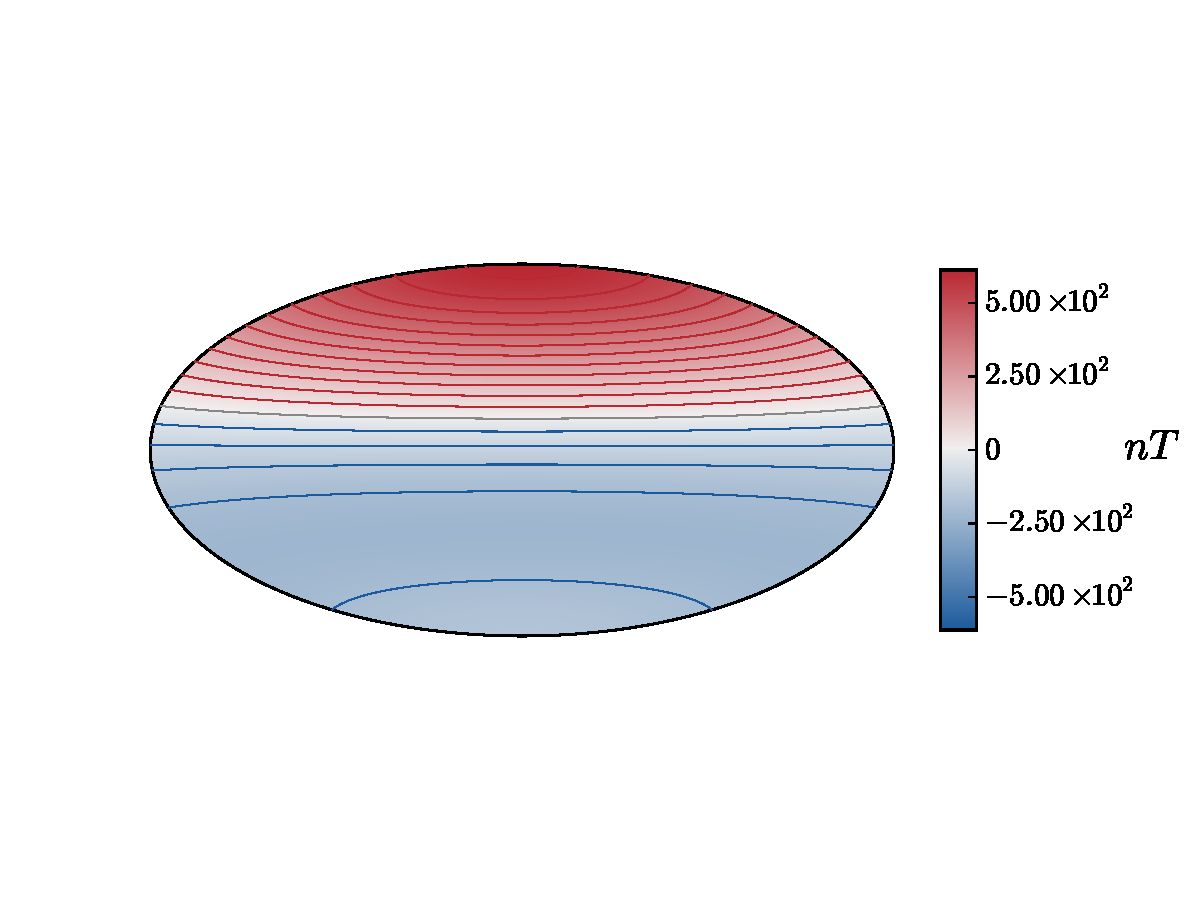
\includegraphics[width=\textwidth]{Chapter1/Figures/Mercury.pdf}
                \caption{Mercury \citep{anderson2012}}
                \label{fig:Mercurybrintro}
        \end{subfigure}
        	 \begin{subfigure}[b]{0.47\textwidth}
                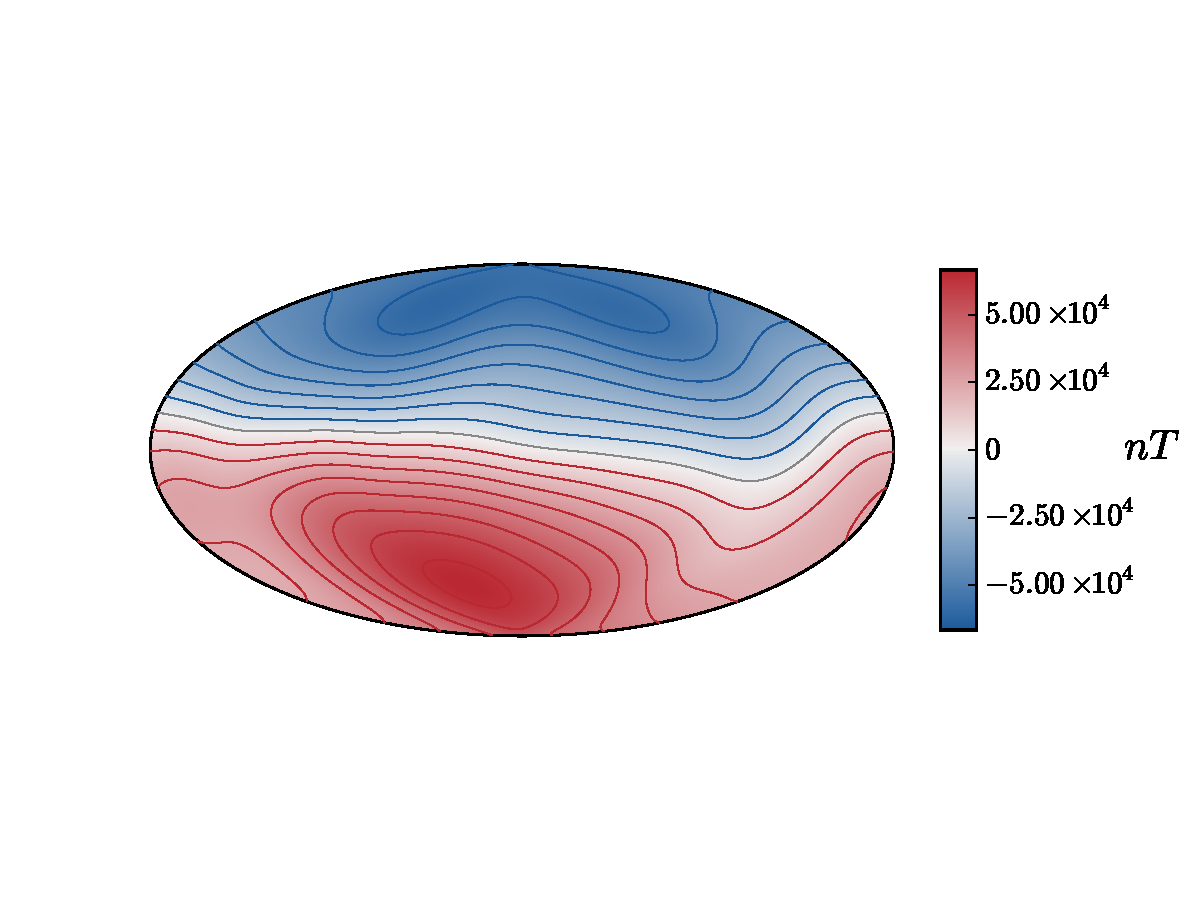
\includegraphics[width=\textwidth]{Chapter1/Figures/Earth.pdf}
                \caption{Earth \citep{igrf11}}
                \label{fig:Earthbr}
        \end{subfigure}
        	\begin{subfigure}[b]{0.47\textwidth}
                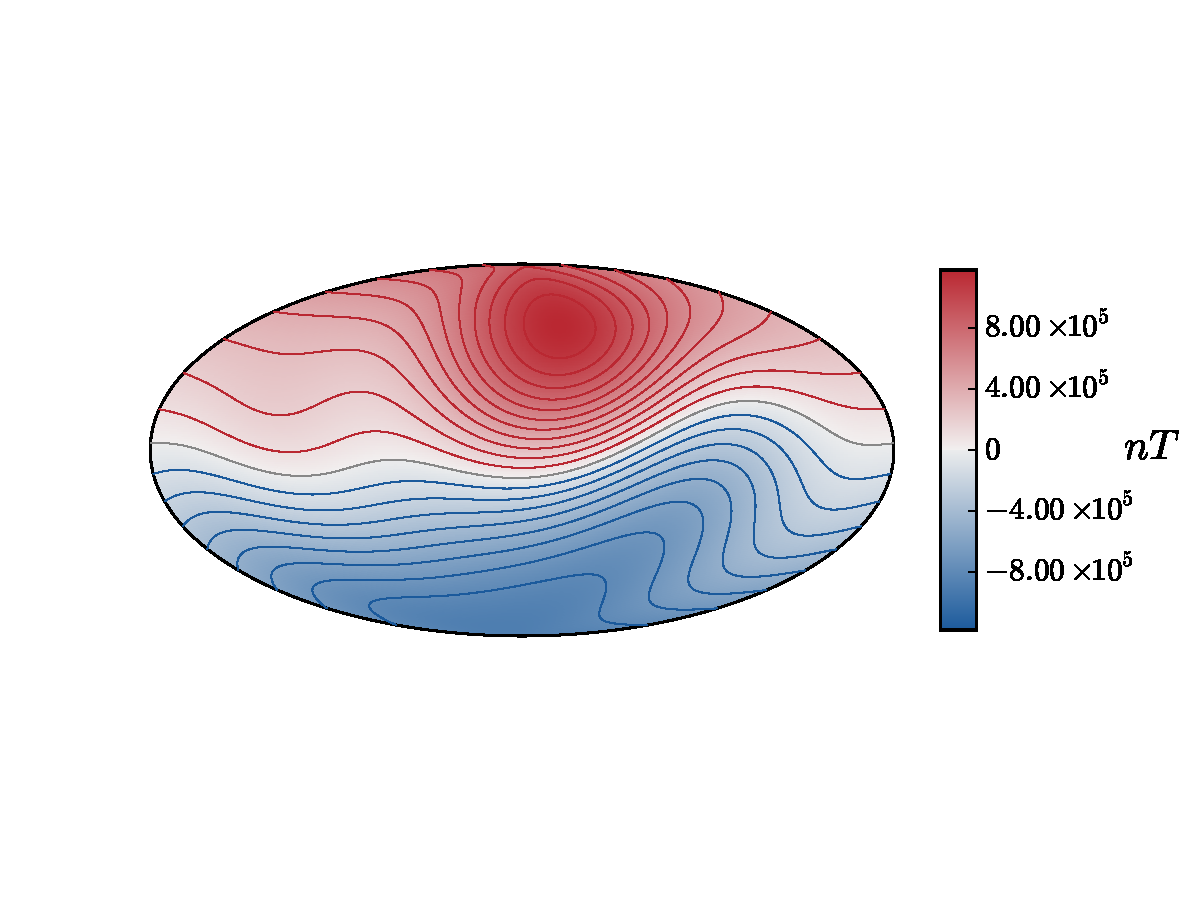
\includegraphics[width=\textwidth]{Chapter1/Figures/Jupiter.pdf}
                \caption{Jupiter \citep{connerney1992}}
                \label{fig:Jupiterbr}
        \end{subfigure}
        	\begin{subfigure}[b]{0.47\textwidth}
                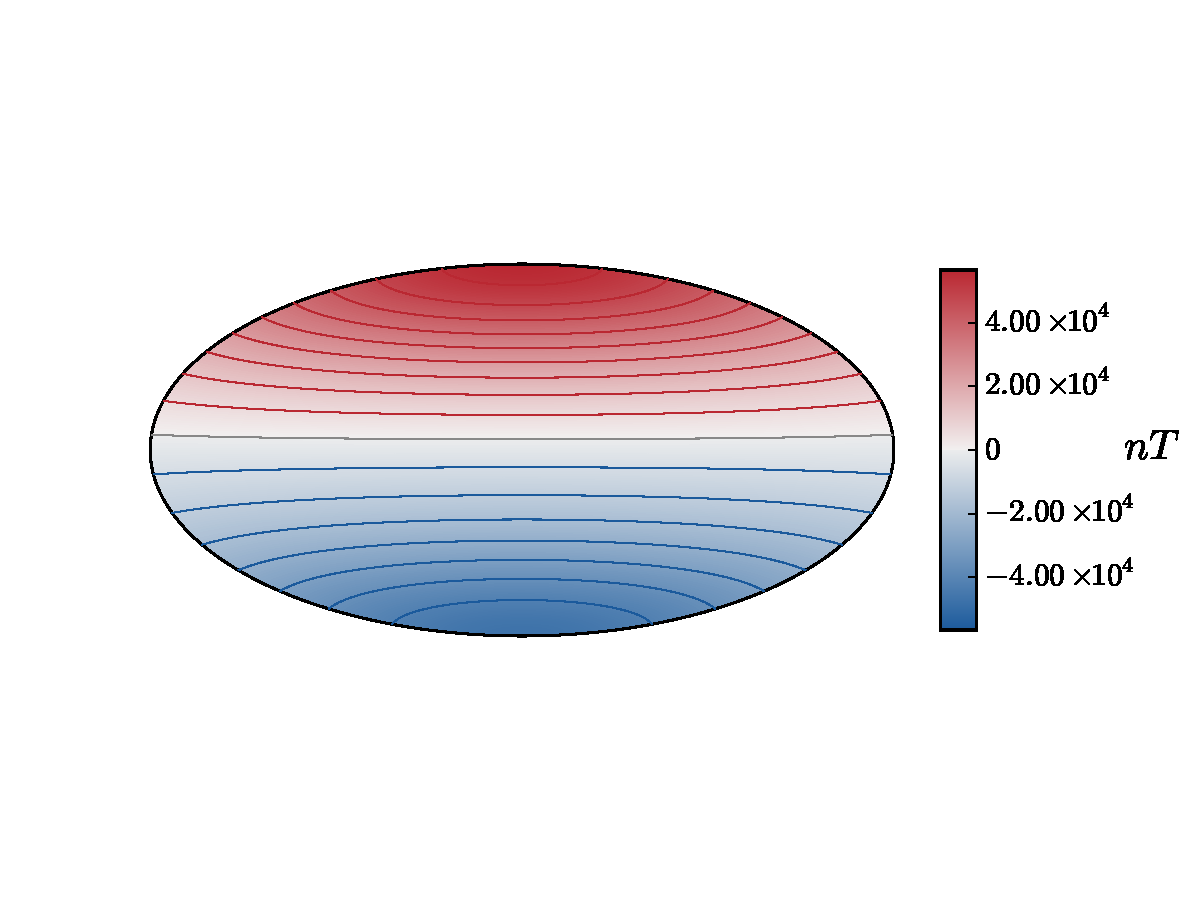
\includegraphics[width=\textwidth]{Chapter1/Figures/Saturn.pdf}
		\caption{Saturn \citep{cao2011}}
                \label{fig:Saturnbr}
        \end{subfigure}
        	\begin{subfigure}[b]{0.47\textwidth}
                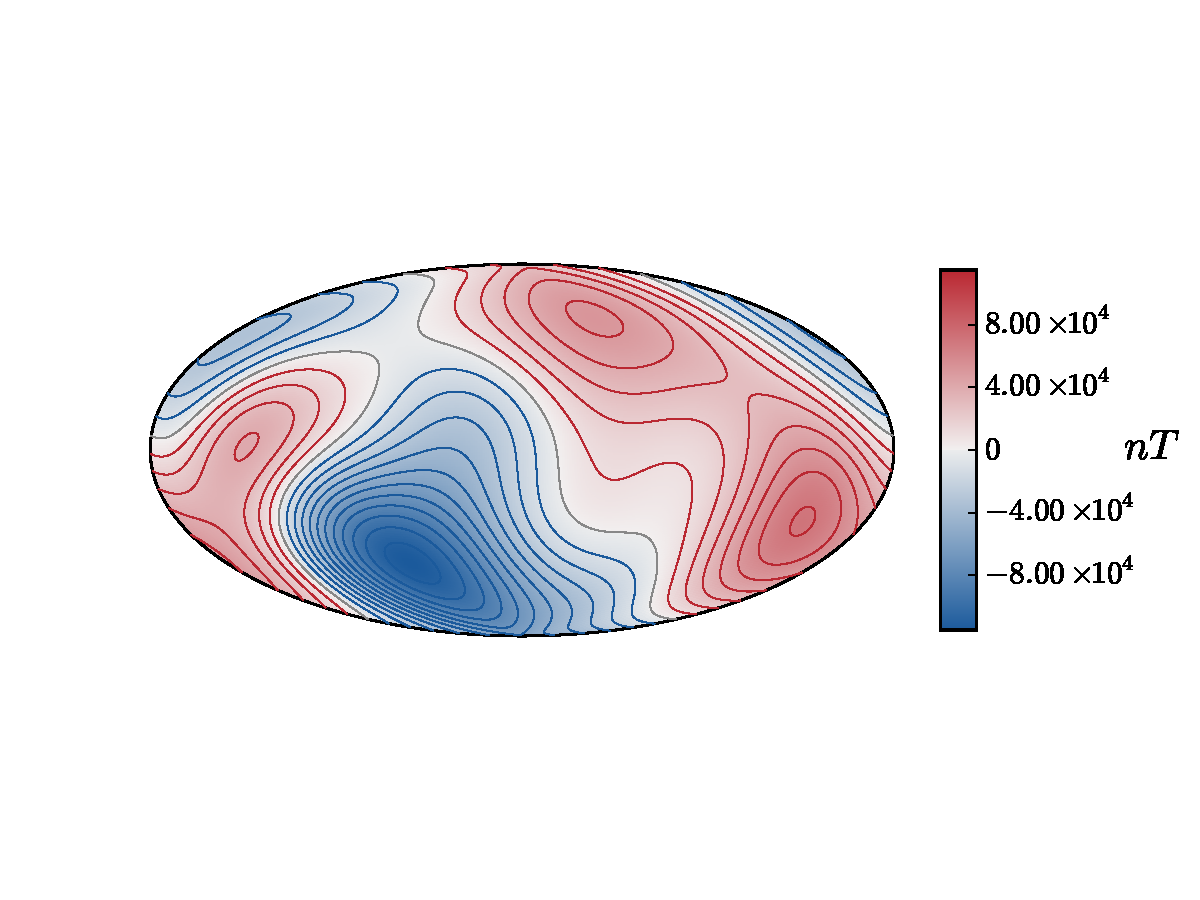
\includegraphics[width=\textwidth]{Chapter1/Figures/Uranus.pdf}
                \caption{Uranus \citep{holme1996}}
                \label{fig:Uranusbr}
        \end{subfigure}
        	\begin{subfigure}[b]{0.47\textwidth}
                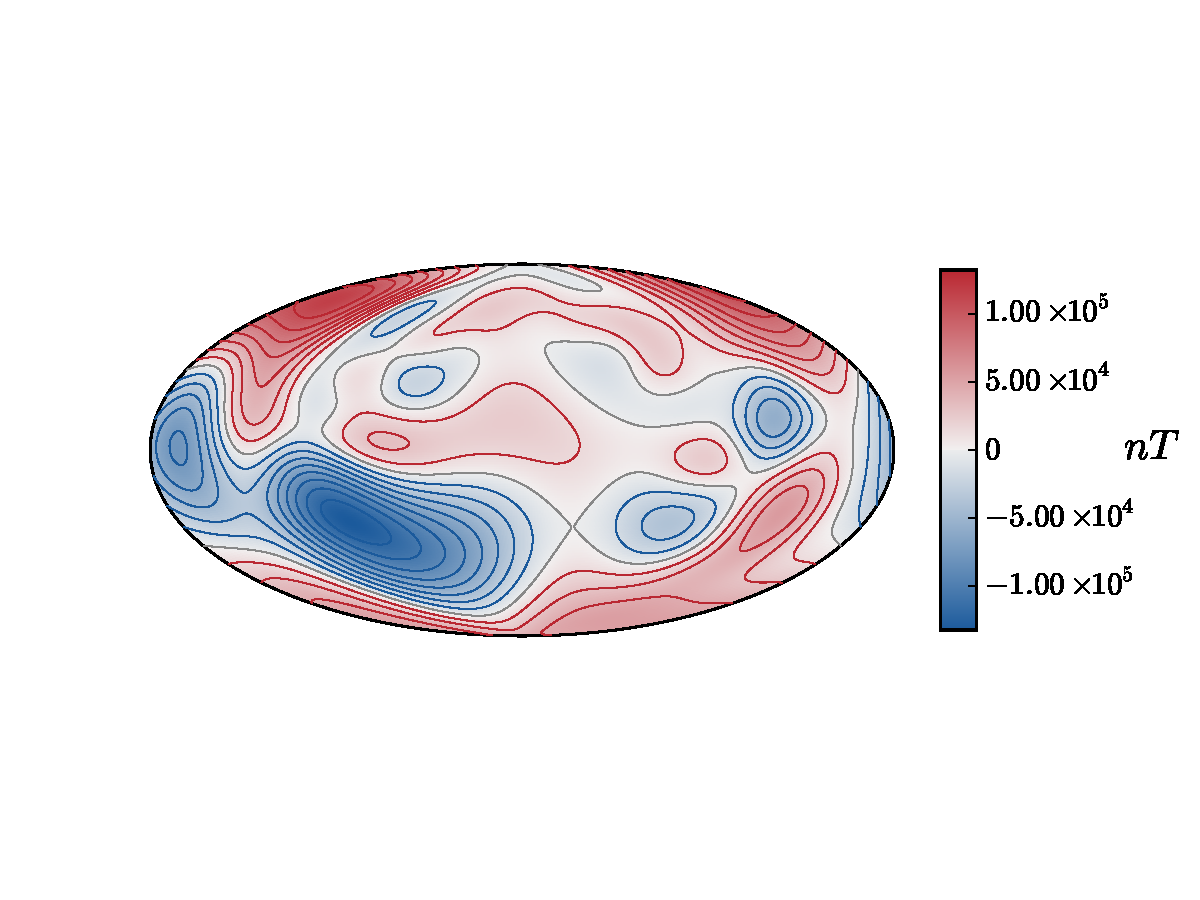
\includegraphics[width=\textwidth]{Chapter1/Figures/Neptune.pdf}
                \caption{Neptune \citep{holme1996}}
                \label{fig:Neptunebr}
        \end{subfigure}
        \caption{The radial magnetic field for each planet in our solar system at the planetary surface.}
\end{figure}

This wide range of planetary magnetic field morphologies generated by active dynamos indicates several important concepts about planetary magnetic fields. First, it shows that dynamos are very sensitive to the geophysical context in which they find themselves. The most striking example of this is the difference between Venus and Earth. Despite the many similarities between these planets (size and composition being foremost among them), Earth has possessed an active dynamo for at least 3.4 billion years \citep{tarduno2010} whereas we have no evidence that Venus ever possessed an active dynamo \citep{russell1980}. Conversely, Jupiter and Earth are dissimilar by most metrics, yet both generate predominantly dipolar magnetic fields that are morphologically similar (figures \ref{fig:Earthbr} and \ref{fig:Jupiterbr}). 

Secondly, this diversity shows that there are many different ``types'' of planetary magnetic fields which share a common mechanism of generation. It is not unreasonable to assume that there are even more classes of dynamos which are not represented in our solar system, because of the small number of planets this system possesses.

In the last decade, ground based observations and the Kepler spacecraft have found hundreds of exoplanets around other stars \citep{rein2015}. These newly discovered planets possess a range of physical properties (e.g. pressures, temperatures \citep{seager2007, valencia2006}, and  compositions \citep{elkins2008, elkins2008coreless}) that are much more diverse and extreme than the physical properties of the planets within our solar system. This naturally raises the question of how the exotic physical properties of exoplanets could affect the existence, detectability and morphology of the dynamos they may possess. 

Of particular interest is the class of terrestrial planets with a mass greater than that of Earth, ``super-Earth's''. These planets are interesting because the pressures and temperatures which must exist in them are not found in any terrestrial body in our solar system. These extreme pressures mean that the constituent materials can behave much differently than they do at the lower pressures within the terrestrial planets of our own solar system \citep{karato2011}. 

This work will focus on testing the effects of novel material properties and solidification regimes on magnetic field generation. First we focus on two ways of reproducing the anomalously weak magnetic field observed at the planet Mercury. These mechanisms use results from high pressure mineralogy and from gravity surveys of Mercury from the recent MESSENGER spacecraft. In the second part we use results from theoretical and experimental high pressure mineralogy to predict the effect of mantle metallization on exoplanetary magnetic fields. 
%!TEX root = ../thesis.tex

\chapter{Dynamo Theory}
\label{chap:dynamotheory}
In its most basic form a dynamo is an engine which takes kinetic energy in the form of fluid motion and transforms it into magnetic energy. In many planetary cores this kinetic energy originates from thermal convection driven by the removal of heat from the core, however other sources of energy such as tidally \citep{cebron2014}, or precessionally driven flows \citep{tilgner2005} are possible. The physical mechanism by which this transfer from kinetic to magnetic energy occurs is summarised in the magnetic induction equation (section \ref{sec:magneticinduction}). 

\section{Maxwells Equations in Planetary Dynamos}
In order to see how dynamos turn fluid velocities into magnetic fields, we must first start with the basic laws concerning electricity and magnetism. The governing equations for this are Maxwell's equations:

\begin{equation}
\nabla \cdot \mbf{E}=\frac{\rho}{\epsilon_{o}}
\label{eq:gauss}
\end{equation}

\begin{equation}
\nabla \cdot \mbf{B}=0
\label{eq:monopoles}
\end{equation}

\begin{equation}
\nabla \times \mbf{B}=\mu_{o} \left(\mbf{J}+\epsilon_{o}\frac{\partial \mbf{E}}{\partial t}\right)
\label{eq:amperesfull}
\end{equation}

\begin{equation}
\nabla\times\mbf{E}=-\frac{\partial \mbf{B}}{\partial t}.
\label{eq:faraday}
\end{equation}
Where $\mbf{B}$ is the magnetic field, $\mbf{J}$ is the current density, $\mbf{E}$ is the electric field, $\rho$ is the charge density, $\epsilon_{o}$ is the electrical permittivity  of free space, and $\mu_{o}$ is the magnetic permeability of free space.

We also use Ohm's law, which relates electric fields to currents:
\begin{equation}
\mbf{J}=\sigma\mbf{E},
\label{eq:ohmslocal}
\end{equation}
where $\sigma$ is the electrical conductivity.

\subsection{The MHD Approximation}
We can approximate Maxwell's equations using the magnetohydrodynamic (MHD) approximation by considering the relative sizes of various terms. First we approximate equation \ref{eq:amperesfull} by comparing the terms $\nabla\times\mbf{B}$ and $\mu_{o}\epsilon_{o} \frac{\partial \mbf{E}}{\partial t}$:
\begin{equation}
\frac{\mu_{o}\epsilon_{o} \frac{\partial \mbf{E}}{\partial t}}{\nabla\times\mbf{B}}.
\end{equation}
Using Faraday's law (equation \ref{eq:faraday}) and characteristic scales for electric field, magnetic field, length and time ($E$, $B$, $L$ and $\tau$ respectively) we can scale $\mbf{E}\sim B L/\tau$ and using $\nabla\times\mbf{B}\sim B/L$ we get
\begin{equation}
\frac{\mu_{o} \epsilon_{o} L^2}{\tau^2}.
\end{equation}
If we take $\mbf{U}\sim L/\tau$ as a characteristic velocity and note that $1/\sqrt{\mu_{o}\epsilon_{o}}$ is the speed of light this becomes
\begin{equation}
\frac{\mu_{o}\epsilon_{o} \frac{\partial \mbf{E}}{\partial t}}{\nabla\times\mbf{B}}\sim\frac{U^2}{c^2}
\end{equation}
meaning the term $\mu_{o}\epsilon_{o} \frac{\partial \mbf{E}}{\partial t}$ is negligible for velocities much less than the speed of light. Since the characteristic velocity in planetary cores is $\mathcal{O}\left(10^{-4}\right) \textrm{m/s} \ll c$ we can safely discard this term in planetary dynamos giving 
\begin{equation}
\nabla \times \mbf{B}=\mu_{o}\mbf{J}.
\label{eq:amperes}
\end{equation}

Next we consider how fields transform between reference frames. We would like to frame our problem in the rotating reference frame of the planetary surface. However in a convecting system each parcel of fluid is moving with respect to the surface at any given time. This means that the quantities present in Maxwell's equations will vary for each parcel of fluid depending on the fluid's velocity with respect to the planetary surface reference frame. It is helpful to reformulate these equations in terms of the $\mbf{E}$, $\mbf{B}$, and $\mbf{J}$ fields that are measured in the planetary surface reference frame. We will denote the reference frame following the fluid as $A^\prime$, all quantities measured in that frame will be distinguished with primes as well. Quantities in the reference frame of the planetary surface will be unprimed. 

If we reformulate the Lorentz transformations in \citet{jackson1999} into components that are parallel ($\parallel$) and perpendicular ($\perp$) to the motion of the $A^\prime$ frame we get:
\begin{align}
\begin{split}
\mbf{E}_{\parallel}^\prime= {} & \mbf{E}_{\parallel}\\
\mbf{B}_{\parallel}^\prime= {} & \mbf{B}_{\parallel}\\
\mbf{J}_{\parallel}^\prime= {} & \gamma\left(\mbf{J}_{\parallel}-\rho\mbf{u}\right)\\
\end{split}
\begin{split}
\mbf{E}_{\perp}^\prime= {} & \gamma\left(\mbf{E}_{\perp}+\mbf{u}\times\mbf{B}_{\perp}\right)\\
\mbf{B}_{\perp}^\prime= {} & \gamma\left(\mbf{B}_{\perp}-\frac{1}{c^2}\mbf{u}\times\mbf{E}_{\perp}\right)\\
\mbf{J}_{\perp}^\prime= {} & \mbf{J}_{\perp}\\
\end{split}
\end{align}
where the velocity relative to the planetary surface frame is $\mbf{u}$ and 
\begin{align}
\gamma=\frac{1}{\sqrt{1-\frac{u^2}{c^2}}}.
\end{align}
For $u\ll c$ we can see that $\gamma\sim 1$. If we use the scaling $E\sim B U$ as before, and scale $\rho u\sim \epsilon_{o} \mu_{o} J L/\tau=J U/c^2$ (equations \ref{eq:faraday}, \ref{eq:gauss}, and \ref{eq:amperes}) these equations reduce to
\begin{align}
\mbf{E}^{\prime} = {} & \mbf{E}+\mbf{u}\times\mbf{B} \label{eq:lorentze} \\
\mbf{B}^{\prime} = {} & \mbf{B} \label{eq:lorentzb} \\
\mbf{J}^{\prime} = {} & \mbf{J} \label{eq:lorentzj}.
\end{align}
We now turn our attention to the Lorentz force. For a continuous charge distribution this is
\begin{equation}
\mbf{F}= \rho \mbf{E} + \mbf{J}\times\mbf{B}
\end{equation}
however using Maxwell's equations to scale $\mbf{E}$ as 
\begin{equation}
E\sim \frac{BL}{\tau} 
\label{eq:escale}
\end{equation}
and use equations \ref{eq:gauss}, \ref{eq:amperes}, and \ref{eq:escale} to show
\begin{align}
\frac{\rho \mbf{E}}{\mbf{J}\times\mbf{B}} = {} & \frac{\left| \epsilon_{0} \mbf{E} \nabla \cdot \mbf{E} \right|}{\left|\nabla\times\mbf{B} \times \mbf{B} /\mu_{o}\right|}\\
\sim {} & \epsilon_{0}\mu_{0} \frac{ E^{2} } { B^{2}  } \\
\sim {} & \frac{u^2}{c^2}\ll1
\end{align}
so the Lorentz force becomes $\mbf{F}=\mbf{J}\times\mbf{B}$.

The final equation we need to consider is Ohm's law (equation \ref{eq:ohmslocal}). This equation is valid for the reference frame of a fluid parcel, not for the planet centred reference frame in which we would like to frame our problem. In the notation of our Lorentz transformations Ohm's law would be written as 
\begin{equation}
\mbf{J}^\prime=\sigma \mbf{E}^{\prime}.
\end{equation}
We can very easily transform this to our planetary surface frame using the approximate Lorentz transformations we just described (equations \ref{eq:lorentze} and \ref{eq:lorentzj}):
\begin{equation}
\mbf{J}=\sigma \left(\mbf{E}+\mbf{u}\times\mbf{B}\right).
\label{eq:ohms}
\end{equation}

\section{Magnetic Induction}
\label{sec:magneticinduction}
In order to see how the transfer of mechanical to magnetic energy occurs we start with Faraday's  law, Amp\`eres law,  and Ohm's law (equations \ref{eq:faraday}, \ref{eq:amperes} and \ref{eq:ohms} respectively). We can put these equations into a more intuitive and convenient form by some simple vector calculus. Taking the curl of Ohm's law (equation \ref{eq:ohms}):
\begin{equation}
\nabla\times\mbf{J}=\sigma \left(\nabla\times\mbf{E}+\nabla\times\left(\mbf{u}\times\mbf{B}\right)\right).
\end{equation}
If we substitute $\mbf{J}$ from equation \ref{eq:amperes} and $\nabla\times\mbf{E}$ from equation \ref{eq:faraday} and rearrange slightly this becomes
\begin{equation}
\frac{\partial \mbf{B}}{\partial t}=\nabla\times\left(\mbf{u}\times\mbf{B}\right)-\frac{1}{\mu_o \sigma}\nabla\times\nabla\times\mbf{B}.
\end{equation}
We can then use the vector identity $\nabla\times\nabla\times\mbf{B}=\nabla\left(\nabla\cdot\mbf{B}\right) -\nabla^{2}\mbf{B}$ along with the fact that magnetic fields are divergenceless to get the magnetic induction equation:
\begin{equation}
\label{eq:dimensionalmagnetic}
\frac{\partial \mbf{B}}{\partial t} = \nabla\times\left(\mbf{u}\times\mbf{B}\right) +\eta \nabla^{2}\mbf{B},
\end{equation}
here we have introduced a quantity known as the magnetic diffusivity ($\eta=1/\sigma \mu_{o}$). This equation relates fluid velocities ($\mbf{u}$) and magnetic fields ($\mbf{B}$) to the time rate of change of the magnetic field. This provides a mechanism by which a planet can  generate a magnetic field. 

%The toroidal and poloidal decomposition we discussed earlier becomes particularly useful now because of the form of equation \ref{eq:dimensionalmagnetic}. If we decompose this equation with the toroidal-poloidal expansion in spherical coordinates to write two scalar evolution equations, we find that the linear parts (the time derivative and the diffusive term) of the equations are independent of each other, and that the only coupling between them is in the inductive term.

\subsection{Interpreting the Magnetic Induction Equation}
\subsubsection{Frozen Flux Theorem and Connections to Fluid Mechanics}
\label{sec:frozenflux}
While the details of the magnetic induction equation (equation \ref{eq:dimensionalmagnetic}) are somewhat opaque, its terms can be interpreted relatively easily. On the right hand side the term $\eta \nabla^{2} \mbf{B}$ is a diffusive term, indicating that magnetic field can diffuse away via ohmic dissipation. The other term, $\nabla\times\left(\mbf{u}\times\mbf{B}\right)$, is less straightforward, but clearly represents interactions between the velocity and magnetic fields. In order for the magnetic field to grow in time, this must be a generation term which is larger than the diffusive term. The relative size of magnetic field generation to diffusion  can be approximately quantified by the magnetic Reynolds number ($\textrm{Re}_{M}$), which is a non-dimensional number found by taking the ratio of these two terms:
\begin{equation}
\textrm{Re}_{M}= \frac{\nabla\times\left(\mbf{u}\times\mbf{B}\right)}{\eta \nabla^{2}\mbf{B}}\sim \frac{UL}{\eta}.
\end{equation}
While it may seem intuitive that $\textrm{Re}_{M}> 1$ should result in magnetic field growth in excess of diffusion, the largest known theoretical lower bound for magnetic field generation is $\textrm{Re}_{M}\sim10$ \citep{BackusBound,ProctorBound}. This is a necessary, but not sufficient condition for magnetic field generation. In numerical dynamo models, magnetic Reynolds numbers on the order of 40 are typical lower bounds  \citep{OlsonandChristensen2006}.

Some intuition about how the magnetic induction equation behaves comes from using the vector identity $\nabla\times\left(\mbf{A}\times\mbf{B}\right)=\mbf{A}\left(\nabla\cdot\mbf{B}\right)-\mbf{B}\left(\nabla\cdot\mbf{A}\right)+\left(\mbf{B}\cdot\nabla\right)\mbf{A}-\left(\mbf{A}\cdot\nabla\right)\mbf{B}$, the divergenceless property of magnetic fields  ($\nabla \cdot \mbf{B}=0$) and by assuming fluid incompressibility\footnote{$\nabla\cdot\mbf{u}=0$, see section \ref{sec:fluidflow} for more information on this approximation.}. With appropriate manipulation equation \ref{eq:dimensionalmagnetic} becomes
\begin{equation}
\frac{\partial \mbf{B}}{\partial t} +\mbf{u}\cdot\nabla\mbf{B}=\mbf{B}\cdot\nabla \mbf{u}+\eta\nabla^{2}\mbf{B}.
\end{equation}
In the limit of infinite electrical conductivity (or zero magnetic diffusivity) this equation becomes
\begin{align}
\frac{\partial \mbf{B}}{\partial t} +\mbf{u}\cdot\nabla\mbf{B}= & {} \mbf{B}\cdot\nabla \mbf{u}\\
\frac{D \mbf{B}}{D t}=& {}\mbf{B}\cdot\nabla \mbf{u}
\label{eq:mievort}
\end{align}
where $D/Dt$ is the advective derivative of fluid mechanics. This equation has the same form as the well known barotropic vorticity equation of atmospheric dynamics. A consequence of that equation is that the vorticity is frozen into the fluid \citep{Vallis}. This is also true of magnetic fields in the magnetic induction equation with an infinite electrical conductivity (zero magnetic diffusivity). In magnetohydrodynamics, this is widely known as the ``frozen flux'' theorem.

We can expand one component (we will choose the $x$ component) of equation \ref{eq:mievort} to get
\begin{equation}
\frac{D B_{x}}{Dt}=B_{x}\frac{\partial u_{x}}{\partial x}+B_{y}\frac{\partial u_{x}}{\partial y}+B_{z}\frac{\partial u_{x}}{\partial z}.
\end{equation}
We can interpret each of these terms as either stretching or tilting magnetic field. The second and third are ``tilting'' terms that tell us that we can increase the magnetic field strength in the $x$-direction by re-orienting magnetic field that is in the $y$- or $z$-directions as long as $u_x$ varies in those directions. The first term is the ``stretching'' term in the magnetic induction equation. This tells us that  spatial gradients of $u_x$ in the $x$-direction can stretch the component of the magnetic field which is co-linear with the velocity. 

\section{Fluid Flow in Planetary Cores}
\label{sec:fluidflow}
The flows in planetary cores are governed by the Navier-Stokes equation modified with the appropriate forces. In its most general form this is
\begin{equation}
\rho\left(\frac{\partial}{\partial t}+\mbf{u}\cdot\nabla\right)\mbf{u}=-\nabla p +\nabla\cdot\mbf{T}+\mbf{F},
\label{eq:navierstokesgeneral}
\end{equation}
here $\rho$ is the fluid density, $p$ is the pressure gradient, $\mbf{T}$ is the deviatoric stress tensor representing shear forces, and $\mbf{F}$ represents body forces.

In Earth's core there are three body forces which are generally used in geodynamo models. These include the Coriolis and Lorentz forces which represent the apparent force of rotation and  magnetic fields respectively, as well as the gravitational force, which allows free convection to occur. Adding these to equation \ref{eq:navierstokesgeneral} gives
\begin{equation}
\rho\left(\frac{\partial}{\partial t}+\mbf{u}\cdot\nabla\right)\mbf{u}+2\rho\mbf{\Omega}\times\mbf{u}=-\nabla p +\mbf{J}\times\mbf{B}+\rho \mbf{g}+\nabla\cdot\mbf{T}
\label{eq:navierstokesgeneralcorlor}
\end{equation}
where $\mathbf{g}$ is the acceleration due to gravity and $\mbf{\Omega}$ is the planetary rotation vector. This equation can be closed by the addition of a conservation of mass equation:
\begin{equation}
\frac{\partial \rho}{\partial t}=\nabla\cdot\left(\rho \mbf{u}\right).
\label{eq:conservationofmass}
\end{equation}
The liquid in the cores of terrestrial planets is mostly iron which is relatively incompressible, and therefore does not exhibit large density variations. A na{\"i}ve approximation would be to neglect all density variations in our fluid. This would be too rash, as density variations are the cause of thermal and compositional convection, which certainly exists within many planetary cores. To simplify these equations we make use the Boussinesq approximation, which states that density variations can be neglected except when they multiply the acceleration due to gravity. This approximation requires that the typical density variations from a reference density $\rho_0$ are small compared to the reference density ($\Delta \rho\ll \rho_0$). Using values in Earth from PREM \citep{prem} we get an average outer core density as $\rho_0=10.9 \textrm{g}/\textrm{cm}^3$ and a density variation between the top and the bottom of the fluid outer core of $2.26 \textrm{g}/\textrm{cm}^3$. Since $2.26\textrm{g}/\textrm{cm}^3\ll 10.9\textrm{g}/\textrm{cm}^3$ we could conclude that the Boussinesq approximation is valid in the Earth's core.

In terrestrial planets with much larger masses than Earth this approximation is often still valid, despite their significantly larger cores and pressures. Using the interior models of \citet{valencia2007} for GJ 876d, a terrestrial planet with mass $7.5 M_\oplus$ we find that even in the most extreme examples (a completely rocky planet with 80\% of its mass in the core) $\Delta \rho/\rho_{0}\approx 0.5$. This implies that the Boussinesq approximation is valid across a wide range of terrestrial planets. Gas and ice planets are a different case, as gasses and ices are relativel compressible, the Boussinesq approximation is in general not valid within them, and different equations of motion must be used.

Under this approximation, equation \ref{eq:conservationofmass} becomes
\begin{equation}
\nabla\cdot\mathbf{u}=0.
\end{equation}
If we finally assume that the fluid is Newtonian we can represent equation \ref{eq:navierstokesgeneralcorlor} as
\begin{equation}
\rho_{o}\left(\frac{\partial}{\partial t}+\mbf{u}\cdot\nabla\right)\mbf{u}+2\rho_{o}\mbf{\Omega}\times\mbf{u}=-\nabla p +\mbf{J}\times\mbf{B}+\Delta\rho \mbf{g}+\rho_{0}\nu\nabla^{2}\mbf{u}.
\label{eq:dimensionalmomentumgeneralbuoyancy}
\end{equation}
In this equation $\rho_{o}$ is the average fluid density, $\nu$ is the kinematic viscosity, and $\Delta\rho$ is the departure from the average density due to thermal or compositional variations.
\subsection{Interpreting the Momentum Equation}
We can gain some insight into how the momentum equation  behaves by considering different force balances. This involves assuming that various terms in equation \ref{eq:dimensionalmomentumgeneralbuoyancy} balance each other exactly, neglecting all other forces. While this is a crude approximation, it allows us to gain some insight into the general behaviour of dynamos.

\subsection{Geostrophic Balance}
If we neglect magnetic fields temporarily and furthermore assume that viscosity, buoyancy and fluid inertia are small, we get a force balance between the pressure gradient and the Coriolis force:
\begin{equation}
\label{eq:geostrophicbalance}
2\rho_{o}\mbf{\Omega}\times\mbf{u}=-\nabla p.
\end{equation}
Taking the the curl of both sides, and using the incompressibility of our fluid gives
\begin{equation}
\pderiv[1]{\mbf{u}}{z}=0 \label{eq:taylorproudman},
\end{equation}
where we take $\hat{z}$ as a unit vector aligned with the axis of rotation. This result is known as the Taylor-Proudman theorem  \citep{proudman1916,taylor1917} and it implies that the fluid motion is invariant along the axis of rotation telling us that convection in rapidly rotating planets should take on a columnar structure with columns aligned along the rotation axis. A representation of this is shown in figure \ref{fig:rolls}.
\begin{figure}
	\centering
	\noindent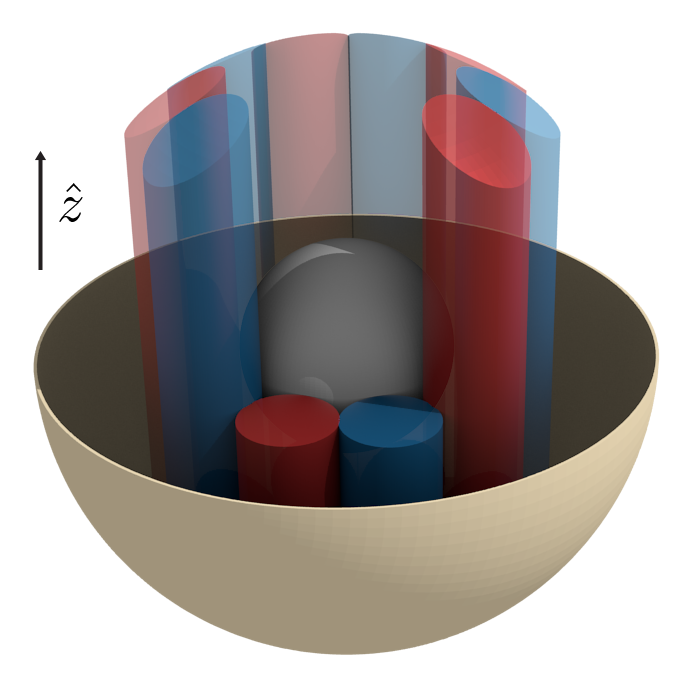
\includegraphics[width=.65\linewidth]{Chapter2/figures/Rolls.png}
	\caption{Convection rolls in an Earth-like core. Red rolls indicate clockwise fluid motion and blue rolls indicate counterclockwise fluid motion. The fluid velocities are invariant along the axis of rotation ($\hat{z}$) due to the Taylor-Proudman theorem. Here the yellow half-sphere is a cutaway of the core-mantle boundary and the grey inner sphere represents the inner core boundary.}
	\label{fig:rolls}
\end{figure}

\subsection{Magnetostrophic Balance}
\label{subsec:magnetostrophic}
If we add magnetic fields to equation \ref{eq:geostrophicbalance} and assume that the Lorentz force balances the Coriolis force and the pressure gradient we get a different expression
\begin{equation}
2\rho_{o}\mbf{\Omega}\times\mbf{u}=-\nabla p + \mbf{J}\times\mbf{B}.
\end{equation}
If we compare the relative strengths of the Coriolis and Lorentz forces we can derive a non-dimensional number known as the Elsasser number 
\begin{align}
\Gamma =& {} \frac{ \mbf{J}\times\mbf{B}}{2\rho_{o}\mbf{\Omega}\times\mbf{u}}\\
 \approx & {} \frac{B^{2}}{2\Omega \eta \rho \mu_{o} }
\end{align}
where $B$ represents a characteristic magnetic field strength and we have taken the magnetic diffusion time ($L^{2}/\eta$) as our characteristic timescale.

This balance is important because if we assume an Elsasser number we can get an estimate of magnetic field strength in the core. An Elsasser number of $\mathcal{O}\left(1\right)$ is a common balance to use, implying all forces besides the Coriolis and Lorentz forces are negligible, and results in a magnetic field strength estimate of $B\approx\sqrt{2\Omega \eta \rho \mu_{o}}$. This balance is called magnetostrophic balance and dynamos which display this are known as strong field dynamos.

\section{Thermal Equation}
The buoyancy force in the momentum equation enters as $\Delta\rho \mbf{g}$ and represents any buoyancy due to compositional or thermal effects. In the planetary dynamo community it is common to combine the effects of temperature and composition into a single variable known as co-density. As they are both important effects in the core, ideally the dynamics of composition and temperature should be solved separately. Each have characteristic diffusivities, which differ by three orders of magnitude \citep{Braginsky1995}, the thermal diffusivity being greater than the compositional diffusivity. In this thesis we adopt the common practice of assuming that small scale (and unresolved) turbulence is present, this acts on both quantities equally and results in an effective turbulent diffusivity which is the same for all quantities. This allows us to introduce the co-density $C$, which is a mixture of compositional and thermal differences with a common  diffusivity due to unresolved turbulence \citep{Braginsky1995, wicht2008}.

The evolution of co-density in the Boussinesq approximation is governed by an energy equation: 
\begin{equation}
\pderiv[1]{C}{t}+\left(\mbf{u}\cdot\nabla\right)C=\kappa \nabla^{2} C + Q\left(r\right).
\label{eq:fullcodensity}
\end{equation}
Here $\kappa$ is the co-density diffusivity and $Q$ represents any co-density sources or sinks within the fluid region. If it is taken to be constant, it often corresponds to a volumetric heat source such as radioactivity, or the evolution of the core's composition due to light element release in compositional convection.
 
We find it convenient to break up the co-density variable into a radially symmetric background state ($C_{o}$) and a perturbation ($\Theta$) which contains the dynamics of the co-density:
\begin{equation}
C=C_{o}\left(r\right)+\Theta\left(\mbf{r},t\right).
\end{equation}
Substituting this definition into equation \ref{eq:fullcodensity} gives
%\frac{\partial C_{o}}{\partial t}+\frac{\partial \Theta}{\partial t}+\left(\mbf{u}\cdot\nabla\right)C_{o}+\left(\mbf{u}\cdot\nabla\right)\Theta=\kappa\nabla^{2}C_{o}+\kappa\nabla^{2}\Theta +Q\left(r\right)
\begin{equation}
\pderiv[1]{C_{o}}{t}+\pderiv[1]{\Theta}{t}+\left(\mbf{u}\cdot\nabla\right)C_{o}+\left(\mbf{u}\cdot\nabla\right)\Theta=\kappa\nabla^{2}C_{o}+\kappa\nabla^{2}\Theta +Q\left(r\right)
\end{equation}
This equation can be separated into two equations, one of which involves only $C_{o}$ and $Q$, while the other contains $\Theta$ and $\mbf{u}$:
\begin{equation}
\pderiv[1]{\Theta}{t}+\left(\mbf{u}\cdot\nabla\right)\left(\Theta+C_{o}\left(r\right)\right)=\kappa \nabla^{2} \Theta\label{eq:dimensionalcodensity}
\end{equation}
\begin{equation}
\kappa\nabla^{2}C_{o}\left(r\right)=-Q\left(r\right).
\label{eq:dimensionalbgcodensity}
\end{equation}
Here equation \ref{eq:dimensionalcodensity} corresponds to the evolution equation for the co-density perturbation and equation \ref{eq:dimensionalbgcodensity} corresponds to the ODE defining the background co-density state. This formalism has a number of advantages, chief among which is that the background state can satisfy the non-homogeneous boundary conditions this problem poses, leaving the evolution equation with relatively simple boundary conditions.

\subsection{Co-Density in the Momentum Equation}
This definition of co-density influences our interpretation of the buoyancy term in the momentum equation. It becomes:
\begin{equation}
\Delta\rho \mbf{g} = \alpha g C \mbf{r},
\label{eq:dimmombuoyancy}
\end{equation}
where $\alpha$ is the co-density expansion coefficient and $\mbf{r}$ is a radial position vector. This assumes that the gravitational acceleration in a planetary core is directed radially and varies linearly with radius (a result easily derivable from Gauss's law). Substituting our definition of co-density into equation \ref{eq:dimensionalmomentumgeneralbuoyancy} gives:
\begin{equation}
\rho_{o}\left(\frac{\partial}{\partial t}+\mbf{u}\cdot\nabla\right)\mbf{u}+2\rho_{o}\mbf{\Omega}\times\mbf{u}=-\nabla p +\mbf{J}\times\mbf{B}+\alpha g r C_{o}\left(r\right)\mbf{\hat{r}}+\alpha g r \Theta\left(\mbf{r},t\right)\mbf{\hat{r}}+\rho_{o}\nu\nabla^{2}\mbf{u}.
\end{equation}
We can then define a modified pressure $\widetilde{p}$ such that
\begin{equation}
\nabla\widetilde{p}=\nabla p-\alpha g r C_{o}\left(r\right)\mbf{\hat{r}}
\end{equation}
which simplifies our momentum equation to
\begin{equation}
\rho_{o}\left(\frac{\partial}{\partial t}+\mbf{u}\cdot\nabla\right)\mbf{u}+2\rho_{o}\mbf{\Omega}\times\mbf{u}=-\nabla \widetilde{p} +\mbf{J}\times\mbf{B}+\alpha g r \Theta\mbf{\hat{r}}+\rho_{o}\nu\nabla^{2}\mbf{u}.
\label{eq:dimensionalmomentum}
\end{equation}
\section{Non-Dimensionalization}
\begin{figure}
	\centering
	\noindent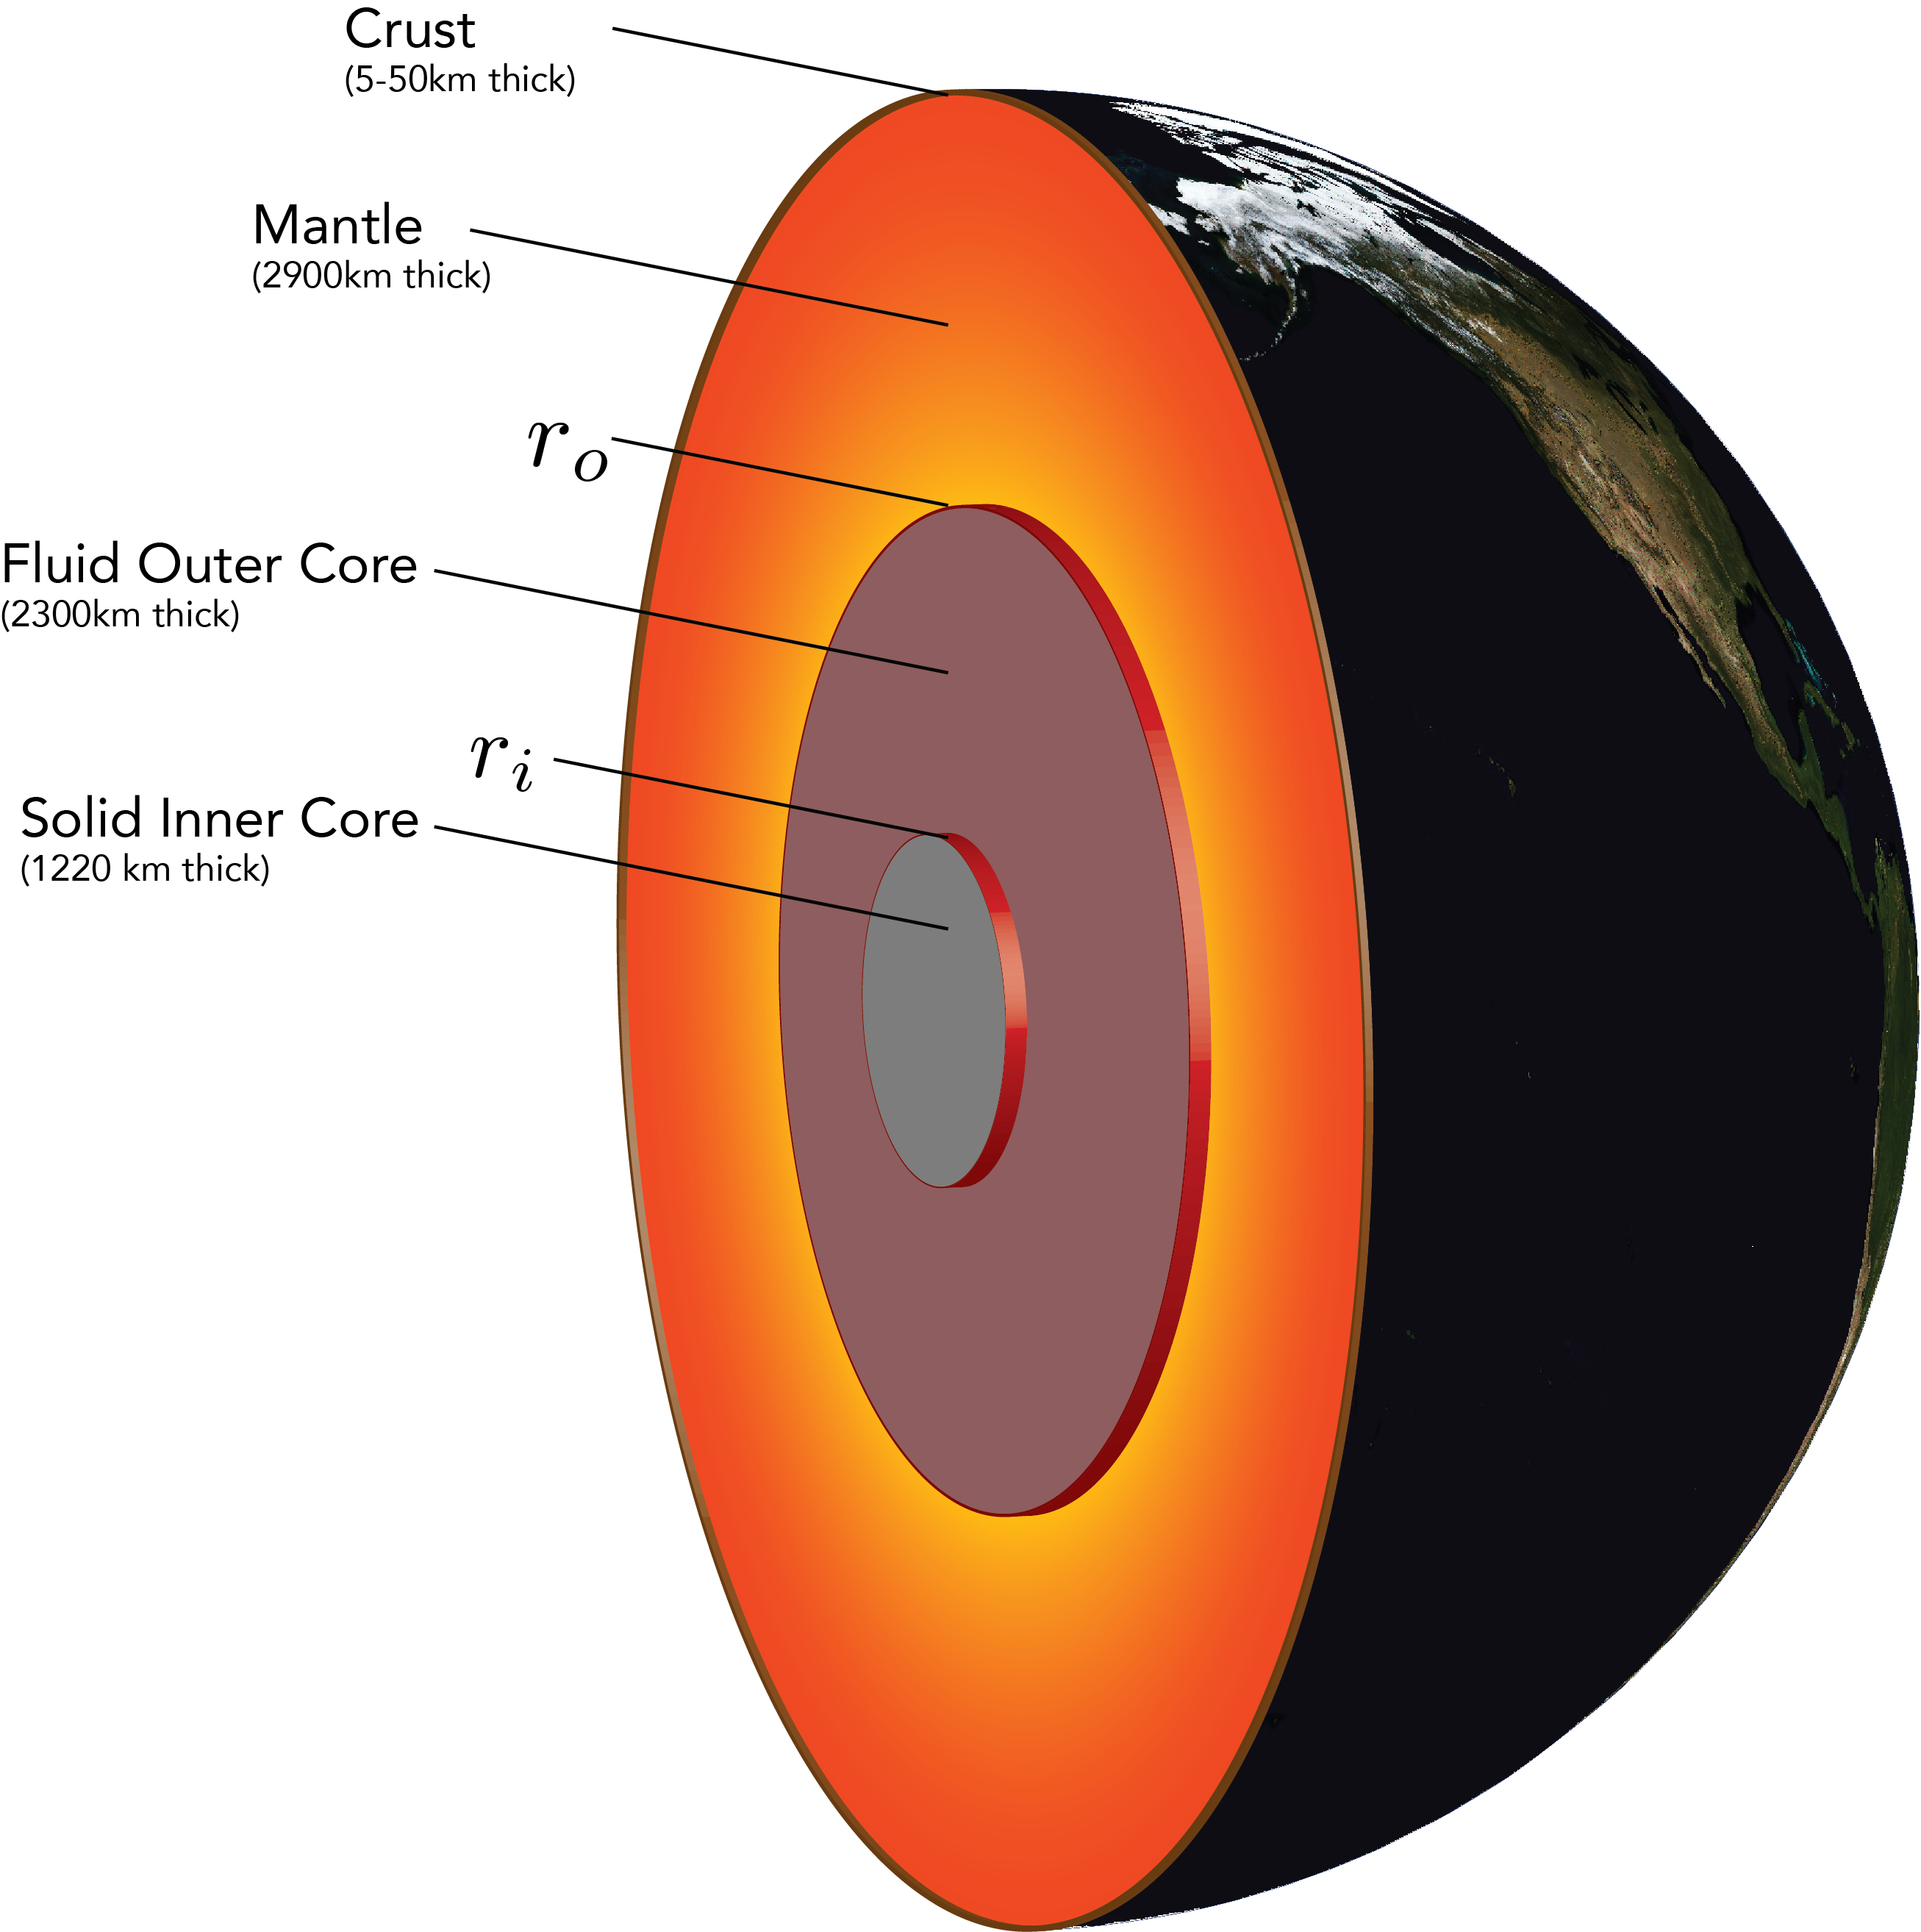
\includegraphics[width=.6\linewidth]{Chapter2/figures/CutawayEarth.png}
	\caption{A cutaway view of the structure of Earth.}
	\label{fig:CutawayEarth}
\end{figure}
We wish to solve the momentum and co-density equations (equations \ref{eq:dimensionalcodensity}, \ref{eq:dimensionalbgcodensity}, and \ref{eq:dimensionalmomentum} ) in a spherical shell. This corresponds to the core of a planet with a solid inner core of radius $r_i$, and a rigid upper boundary of radius $r_o$ (see figure \ref{fig:CutawayEarth}). 

If we are to non-dimensionalise our equations we would like to pick units which have a physical relevance to the problem we wish to solve. For this reason we choose the outer core radius ($r_{o}$) as our length scale and choose the magnetic diffusion time $\tau=r_{o}^{2}/\eta$ as our timescale. To get a scale for the magnetic field, we follow the method outlined in section \ref{subsec:magnetostrophic} and assume an Elsasser number of 1, giving $B=\sqrt{2\Omega\eta\rho\mu_{o}}$. Finally we choose $h_{C} r_o$ as our co-density scale where $h_{C}$ is the co-density flux at the inner core boundary.

When we apply these non-dimensionalisations, equations \ref{eq:dimensionalmagnetic}, \ref{eq:dimensionalcodensity}, \ref{eq:dimensionalbgcodensity}, and \ref{eq:dimensionalmomentum} become
\begin{align}
Ro\left(\frac{\partial}{\partial t}+\mbf{u}\cdot\nabla\right)\mbf{u}+\mbf{\hat{z}}\times\mbf{u}=& {} -\nabla p+\mbf{J}\times\mbf{B}+Ra\Theta\mbf{r}+E\nabla^{2}\mbf{u} \label{eq:nondimmomentum}\\
\frac{\partial \Theta}{\partial t}+\mbf{u}\cdot\nabla C =& {}q_{\kappa}\nabla^{2}\Theta \label{eq:nondimcodensity}\\
\frac{\partial \mbf{B}}{\partial t}=& {} \nabla\times\left(\mbf{u}\times\mbf{B}\right)\label{eq:nondimmagnetic}+\nabla^{2}\mbf{B}.
\end{align}
The nondimensional parameters in equations (\ref{eq:nondimmomentum}) to (\ref{eq:nondimmagnetic}) are the Rayleigh number ($Ra$), the magnetic Rossby number ($Ro$), the magnetic Prandtl number ($q_{\kappa}$), and the Ekman number ($E$). These are given by:
\begin{align}
Ra=& {}\frac{\alpha g_{o}h_{C}r_{o}^{2}}{2\Omega\eta} \label{eq:rayleigh}\\
Ro=& {}\frac{\eta}{2\Omega r_{o}^{2}}\\
q_{k}=& {}\frac{\kappa}{\eta}\\
E=& {}\frac{\nu}{2\Omega r_{o}^2} \label{eq:ekman}.
\end{align}
The Rayleigh number defined in equation \ref{eq:rayleigh} is a modified Rayleigh number that differs in form from the Rayleigh number used in mantle convection. In non-rotating convection it is useful to define the Rayleigh number as the ratio between buoyancy and viscous forces, as viscosity is often the force that buoyancy must overcome in order for convection to occur. In rotating core convection, viscosity is typically very small, and buoyancy must overcome the ``stiffness'' of the fluid imposed by Taylor-Proudman theorem (equation \ref{eq:taylorproudman}) in order for convection to occur. For this reason we define the Rayleigh number as the ratio between the buoyancy force and the Coriolis force. As the Ekman number (equation \ref{eq:ekman}) is the ratio of the viscous force to the Coriolis force, a more conventional Rayleigh number can be recovered by dividing the modified Rayleigh number by the Ekman number. 


\section{The Local Rossby Number}
\label{sec:rol}
One factor which makes dynamos difficult to understand is the large number of control parameters that are required to specify a solution to the governing equations. This is particularly troubling because the properties of a dynamo are dependent on the values of these control parameters. Unfortunately, for numerical reasons, dynamo models must be run in a parameter regime for which most of the control parameters are not appropriate for modelling planetary cores.

\citet{christensen06scaling} developed a scaling law concerning planetary dynamos which has proved to be useful in the prediction of the bulk properties of a dynamo as a function of its control parameters. The Rossby number is normally defined as the ratio of the inertial force to the Coriolis force, from equation \ref{eq:navierstokesgeneralcorlor} this is
\begin{align*}
Ro&=\frac{\left|\rho \mbf{u}\cdot\nabla\mbf{u}\right|}{\left|2\rho\mbf{\Omega}\times\mbf{u}\right|}\\
&\approx\frac{U}{\Omega r_o}.
\end{align*}
\citet{christensen06scaling} noted that while the inertial term depends on the length scale of the flow, the Coriolis term does not. They posited that a better measure of the role rotation plays in a given flow may be a Rossby number which depends on the characteristic length scale of the flow, rather than the characteristic length scale of the container. They defined this length scale as
\begin{equation}
\label{eq:rollength}
\bar{\ell}_{u}=\frac{4Ro_m^2}{\left(1-r_{io}\right)^2}\frac{\sum l\left\langle\mbf{u}_{l}\cdot\mbf{u}_{l}\right\rangle}{2E_{kin}}
\end{equation}
where $E_{kin}$ is the kinetic energy, defined as
\begin{equation}
E_{kin}=\frac{4 Ro_m^2}{\left(1-r_{io}\right)^{5}}\frac{1}{2}\int_{V}\left(\mbf{u}\cdot\mbf{u}\right)dV
\end{equation}
using the non-dimensionalisation of \citet{kuangandbloxham1999}. The factor in front of the integral results from converting the non-dimensionalisation from those used in \citet{christensen06scaling}. Combining these we get
\begin{equation}
\bar{\ell}_{u}=\left(1-r_{io}\right)^{3}\frac{\sum l\left\langle\mbf{u}_{l}\cdot\mbf{u}_{l}\right\rangle}{\int_{V}\left(\mbf{u}\cdot\mbf{u}\right)dV}.
\end{equation}
Since the mean radius to a point inside the shell is of order one, they set the half wavelength of the flow to $\pi/\ell_u$ giving a local Rossby number of 
\begin{equation}
\label{eq:rol}
Ro_{l}=Ro\frac{\bar{\ell}_{u}}{\pi}.
\end{equation}

\citet{christensen06scaling} then noted that the dipole dominance of the poloidal magnetic field depended strongly on the local Rossby number. They showed that dynamo models which had $Ro_{l}\leq 0.12$ had magnetic fields that were predominantly dipolar, while models with $Ro_{l}>0.12$ generated multipolar magnetic fields. This sharp transition is clear if the dipole dominance of the observable magnetic field ($f_{dip}$) is plotted against the local Rossby number (figure \ref{fig:rolfdip}). Using angle brackets to denote a time average, $f_{dip}$ is defined as
\begin{equation}
f_{dip}=\left\langle\frac{ \int_S \sqrt{\mbf{B}_{l=1}\cdot\mbf{B}_{l=1}} }{\sum_{l=1}^{12} \int_S  \sqrt{\mbf{B}_{l}\cdot\mbf{B}_{l}}}\biggr\rvert_{r=r_{o}}\right\rangle
\end{equation}
which is the time average ratio of the r.m.s. amplitude of the dipole field to the r.m.s. amplitude of the field in the first 12 degrees.
\begin{figure}
	\centering
	\noindent\includegraphics[width=.5\linewidth]{Chapter2/figures/fdip.pdf}
	\caption{The dipole dominance ($f_{dip}$) of the observable magnetic field as a function of the local Rossby number. Here $f_{dip}$ is defined as the time average ratio of the r.m.s. amplitude of the dipole field to the r.m.s. amplitude of the field in the first 12 degrees. The Ekman numbers here are in the variables of \citet{christensen06scaling}; they can be converted to the Ekman numbers in this work by multiplying them by a factor of $0.21125$. This figure is reproduced from \citet{christensen06scaling} where it is figure 3.}
	\label{fig:rolfdip}
\end{figure}

Once the local Rossby number is defined, a natural extension is to apply it to the planets of our solar system. The definition of equation \ref{eq:rol} requires a knowledge the characteristic fluid velocity and scale in the fluid outer core. This is very unconstrained for even Earth, and less well constrained for other planets of our solar system. An alternative approach is to construct scaling laws which relate the control parameters of the dynamo to the local Rossby number. The control parameters depend on the physical properties of the planet (e.g. diffusivities, rotation rates etc.) which are known more accurately than the dynamical properties (i.e. the scale of convection).

Several studies have constructed scaling laws which relate the dynamo control parameters to the local Rossby number \citep{christensen06scaling,OlsonandChristensen2006,aubert2009}. The most general is from \citet{aubert2009}; if it is cast into the non-dimensionalisation used in this work it can be written as
\begin{equation}
Ro_{l}=0.674\frac{1+r_{io}}{\left(1-r_{io}\right)^{-0.64}}p^{0.48}E^{-0.32}q_{\kappa}^{-0.19}.
\label{eq:rolscaling}
\end{equation}
$p$ is the convective power density. Assuming the background state does not change, the convective power density can be written as
\begin{equation}
p=\frac{3}{2}\frac{(1-r_{io})^2}{\left(1-r_{io}^3\right)} \left[(1-f_{i})\left(\frac{1}{(1-r_{io})^2}-\frac{3}{5}\frac{\left(1-r_{io}^5\right)}{\left(1-r_{io}^3\right)}\right)+f_{i} \left(\frac{3}{5}\frac{\left(1-r_{io}^5\right)}{\left(1-r_{io}^3\right)}-\frac{r_{io}^2}{(1-r_{io})^2}\right)\right]Ra_Q
\end{equation}
where $f_i$ is the fraction of the total buoyancy flux injected at the inner core and $Ra_Q$ is a Rayleigh number based on advected buoyancy flux \citep{aubert2009}.

\section{Magnetic Screening by Conductors}
\label{sec:screeningderiv}
Two projects within this thesis will involve the effect of a solid conducting layer placed between the dynamo region and the planetary surface. It is therefore worthwhile to discuss the effect of this layer on the observable magnetic field. In the absence of fluid motion, the magnetic induction equation (equation \ref{eq:dimensionalmagnetic}) becomes a diffusion equation:
\begin{equation}
\pderiv[1]{\mbf{B}}{t}=\eta\nabla^{2}\mbf{B}.
\end{equation}
To illustrate the screening effect we will solve this equation in a cartesian geometry with a constant diffusivity. We will solve this system in a semi-infinite ($z>0$), cartesian geometry, and apply a magnetic field that oscillates with frequency $\omega$ at the finite boundary. In this geometry, this system is described as
\begin{align}
\pderiv[1]{B}{t}= & {}\eta\pderiv[1]{B}{z} \label{eq:conlayerdiffusion} \\
B\left(z=0,t\right)= & {}\sin\left(\omega t\right) \\
B\left(z \to \infty,t\right)= & {} 0
\end{align}
Where $B$ is an arbitrary component of $\mbf{B}$. An ansatz of the form
\begin{equation}
B=B_{0}e^{-\gamma z} \sin\left(kz-\omega t\right)
\label{eq:bansatz}
\end{equation}
satisfies the boundary conditions and implies a wave-like solution that decays to infinity. Substituting equation \ref{eq:bansatz} into equation \ref{eq:conlayerdiffusion} we find  
\begin{equation}
-B_{0}\omega  e^{-\gamma  z} \cos (k z-\omega t  )=\eta B_{0} e^{-\gamma  z} \left[\left(\gamma ^2-k^2\right) \sin (k z- \omega t
    )-2 \gamma  k \cos (k z- \omega t  )\right].
\end{equation}
This implies that a solution requires $\gamma=\pm k, k=\sqrt{\pm \omega / 2 \eta}$. Here we pick the branch which leads to physicsl (real) solutions and finite solutions at infinity. Equation \ref{eq:bansatz} becomes
\begin{equation}
B=B_{0}e^{-\sqrt{\omega/\left(2\eta\right)} z} \sin\left(\sqrt{\frac{\omega}{2\eta}}z-\omega t\right)
\end{equation}
Recasting $\omega$ from a frequency to a timescale ($\tau \sim 1/\omega$) this becomes
\begin{equation}
B=B_{0}e^{-\sqrt{1/\left(2\tau\eta\right)} z} \sin\left(\sqrt{\frac{1}{2\tau \eta}}z-\omega t\right).
\label{eq:conlayerdiffusionsoln}
\end{equation}
Equation \ref{eq:conlayerdiffusionsoln} implies that a magnetic field that varies with timescale $\tau$ decays with a characteristic depth of $\sqrt{2\tau \eta}$. Equivalently, a conducting layer of thickness $d$ will attenuate a magnetic field varying with timescale $\tau$ by a factor of $e^{-\sqrt{1/\left(2\tau\eta\right)} d}$.

\section{Numerically Simulating the Dynamo}
As equations \ref{eq:nondimmomentum}-\ref{eq:nondimmagnetic} have no general analytic solutions we must turn to numerical methods in order to obtained detailed insight into magnetic field generation in planets. To do this we use the Kuang-Bloxham \citep{kuangandbloxham1997, kuangandbloxham1999} and mMoSST \citep{jiang2008} numerical dynamo models. Both of these numerical models solve equations \ref{eq:nondimmomentum}-\ref{eq:nondimmagnetic}, and differ only in the numerical methods they use. 

The most important difference between the Kuang-Bloxham model and the mMoSST model lies in the inertial term. In planetary cores the influence of fluid inertia is expected to be small save for a certain class of axisymmetric waves known as torsional oscillations \citep{dumberry2003}. For numerical reasons, dynamo models cannot currently operate in a region of parameter space that yields a realistically small inertial force, meaning that most dynamo models do not reproduce the correct force balance. The Kuang-Bloxham model attempted to attain the correct force balance in the core while keeping torsional oscillations \citep{kuangandbloxham1999}. In order to reproduce torsional oscillations while attaining the magnetostrophic balance, the non-axisymmetric component of the inertial term in equation \ref{eq:nondimmomentum} was discarded. Although this approximates the momentum equation it may provide a more accurate force balance of planetary cores \citep{dumberry2003}. Despite this approximation the Kuang-Bloxham model has been successfully benchmarked against other numerical dynamo models \citep{dharmaraj2013}. mMoSST has a more subtle way of representing the fluid inertia term in equation \ref{eq:nondimmomentum}. It has the ability to represent the term fully, for all spherical harmonic orders up to a user specified order. When we use the mMoSST model in this work we include the full inertial term for all orders.

\subsection{Boundary Conditions}
Equations \ref{eq:nondimmomentum}-\ref{eq:nondimmagnetic} require boundary conditions to specify unique solutions. Both the Kuang-Bloxham and mMoSST numerical dynamo models are capable of a range of commonly used boundary conditions for each field.
\subsubsection{Velocity Field}
All models presented in this work require the radial component of the velocity field to be zero at the core-mantle, and inner core boundaries. These conditions correspond to  impenetrable conditions, which is appropriate for a solid barrier such as the mantle or the inner core. The tangential velocity requires a more subtle approach. In Earth, a no-slip  condition is the correct velocity boundary at both the inner and outer core as the velocity of the fluid must match the velocity of the solid boundary it meets. 

Computational restrictions require numerical dynamo models to operate in a parameter regime that is very far removed from the regime that is relevant to planetary cores. In particular, the Ekman number used in dynamo models $\mathcal{O}\left( 10^{-5} \right)$ is commonly $10$ orders of magnitude larger than the Ekman number of Earth's core $\mathcal{O}\left(10^{-15}\right)$. Table \ref{tab:ekman} shows approximate Ekman numbers for the the planets of our solar system. These Ekman number are extremely uncertain, mostly because of the viscosity. These estimates use the molecular viscosity of core fluids. It is not clear whether this is the most representative choice, or whether turbulent viscosities may be a better choice. In that case the Ekman numbers will be several orders of magnitude higher than the values reported here
\begin{table}[]
\label{tab:ekman}
\centering
\caption{My caption}
\label{my-label}
\begin{tabular}{lc}
Planet       & \multicolumn{1}{l}{Ekman Number} \\
Mercury      & $\mathcal{O})\left(10^{-12}\right)$                              \\
Venus        & $\mathcal{O})\left(10^{-13}\right)$                              \\
Earth        & $\mathcal{O})\left(10^{-15}\right)$                              \\
Moon         & $\mathcal{O})\left(10^{-12}\right)$                              \\
Mars         & $\mathcal{O})\left(10^{-14}\right)$                              \\
Jupiter      & $\mathcal{O})\left(10^{-18}\right)$                              \\
Ganymede     & $\mathcal{O})\left(10^{-14}\right)$                              \\
UranusSaturn & $\mathcal{O})\left(10^{-17}\right)$                              \\
Uranus       & $\mathcal{O})\left(10^{-16}\right)$                              \\
Neptune      & $\mathcal{O})\left(10^{-16}\right)$                             
\end{tabular}
\end{table}
One effect of a larger than realistic Ekman number is that numerical models overestimate the size of the visco-rotational boundary layers known as Ekman layers. The thickness of these Ekman layers is:

\begin{equation}
d\sim \sqrt{2E} r_{o},
\end{equation}
which corresponds to $15$km at $E=10^{-5}$, but only $15$cm at $E=10^{-15}$. To avoid over representing the size of the Ekman boundary layers and their associated secondary circulation \citep{gubbins2007}, some authors \citep{kuangandbloxham1999} use free slip boundary conditions, which eliminates the viscous coupling between the core and the mantle as well as the associated secondary circulation. The Kuang-Bloxham and mMoSST models are capable of using both stress free and no-slip boundary conditions. 

\subsubsection{Thermal Field}
The thermal boundary conditions commonly used in numerical dynamo models can be grouped into two general categories: fixed flux and fixed temperature boundary conditions. In fixed temperature boundary conditions the co-density is set to a value at the boundary, giving Dirichlet boundary conditions. In fixed flux boundary conditions the derivative of the co-density is set at the boundary, corresponding to a Neumann boundary condition. While many studies use fixed temperature boundary conditions for simplicity reasons, there is some evidence \citep{sakuraba2009} that fixed flux boundary conditions generate more Earth-like magnetic fields as the parameter regime becomes closer to Earth.

\subsubsection{Magnetic Field}
Both the Kaung-Bloxham and mMoSST dynamo models are able to simulate a variety of inner core and solid mantle types. In the models considered within this work, the inner core and mantle layers have a finite, non-zero conductivity. We also allow the inner core and mantle to rotate relative to the rotating, fluid outer core frame of reference, which makes the boundary conditions more complicated as they involve an inductive term due to the relative motion of the solid layer (inner core or the mantle) and the fluid outer core.

If we consider the boundary between two regions (region 1 and region 2) the boundary conditions supplied by Maxwell's equations are:
\begin{align}
 \hat{n}\cdot\mbf{B}^1 &= \hat{n}\cdot\mbf{B}^2 \label{eq:bboundary} \\
 \hat{n}\times\mbf{E}^1 &= \hat{n}\times\mbf{E}^2 \label{eq:eboundary}
\end{align}
where $\hat{n}$ is the unit vector normal to the boundary and a superscript denotes the region number. These imply that the magnetic field is continuous across the boundary in the radial direction while the electric field is continuous across the boundary in the horizontal direction. As planetary cores are very close to spherical, we will take this to be the radial unit vector $\hat{r}$. Beginning with equation \ref{eq:bboundary} it is easy to show that
\begin{equation}
B_r^1=B_r^2.
\end{equation}
The second boundary condition in equation \ref{eq:eboundary} can be expanded into two boundary conditions, one for each component of the resulting vector expression
\begin{align}
E_{\theta}^1=E_{\theta}^2\\
E_{\phi}^1=E_{\phi}^2 .
\end{align}
This expression does not account for the movement of either region with respect to the rest frame of the equations of motion. Each part of the physical system we wish to solve (inner core, fluid outer core, and solid mantle layer) can move with respect to the rest frame of \ref{eq:nondimmomentum}-\ref{eq:nondimmagnetic}. For this reason we would like to recast our boundary conditions in our planetary surface reference frame using the Lorentz transformation (equation \ref{eq:lorentze}). In the case of our general example using regions 1 and 2, we will assume that region 1 moves with velocity $\mbf{u}^1$ and region two moves with velocity $\mbf{u}^2$:
\begin{align}
E_{\theta}^1-\left(\mbf{u}^1\times\mbf{B}^2\right)_\theta=E_{\theta}^2-\left(\mbf{u}^2\times\mbf{B}^2\right)_\theta \\
E_{\phi}^1-\left(\mbf{u}^1\times\mbf{B}^2\right)_\phi=E_{\phi}^2-\left(\mbf{u}^2\times\mbf{B}^2\right)_\phi .
\end{align}
Expanding, and using the non-penetration condition at the boundary ($u_r=0$) we get:
\begin{align}
E_{\theta}^{1}-u_{\phi}^{1}B_{r}^{1}=E_{\theta}^{2}-u_{\phi}^{2}B_{r}^{2}\\
E_{\phi}^{1}+u_{\theta}^{1}B_{r}^{1}=E_{\phi}^{2}+u_{\theta}^{2}B_{r}^{2}.
\end{align}
Finally defining $\llbracket A \rrbracket$ as $A^{1}-A^{2}$, using Ohm's law (equation \ref{eq:ohmslocal}) and $\llbracket B_r \rrbracket=0$ we get:
\begin{align}
\bigg\llbracket \frac{J_{\theta}}{\sigma}\bigg\rrbracket+ \llbracket u_{\phi}\rrbracket B_r= 0 \\
\bigg\llbracket \frac{J_{\phi}}{\sigma}\bigg\rrbracket -\llbracket u_{\theta}\rrbracket B_r= 0.
\end{align}
Our $\llbracket \rrbracket$ operator can now refer to any boundary in our dynamo problem (either the inner-core boundary or the core-mantle boundary).

\subsection{Numerical Methods}

\subsubsection{Discritisation}
Both the Kuang-Bloxham and mMoSST numerical dynamo model approximate equations \ref{eq:nondimmomentum}-\ref{eq:nondimmagnetic} with a mixed spectral-finite difference method. In both models the angular parts of the equations \ref{eq:nondimmomentum}-\ref{eq:nondimmagnetic} are expanded in a truncated spherical harmonic series. For equations \ref{eq:nondimcodensity} and \ref{eq:nondimmagnetic} both models use a compact finite difference method for the treatment of derivatives with respect to r. Compact finite differences are an implicit approach to the calculation of finite differences which allows for greater accuracy (see \citet{lele1992}) The radial grid points are specified at the extremas of Chebyshev polynomials (rescaled from $[-1, 1]$ to $[r_i, r_o]$). As Chebyshev polynomials group their extremas near the boundaries, this concentrates the gridpoints near the boundaries to resolve thin boundary layers. The Kuang-Bloxham and mMoSST models differ in their treatment of the radial derivatives in the momentum equation. In the Kuang-Bloxham model, the momentum equation is treated spectrally in the radial direction using Chebyshev polynomials as a spectral basis function. This follows many other well established dynamo models (e.g. \citet{wicht2002}) and provides good convergence properties at the expense of parallelization. In the mMoSST model, the radial derivatives in the momentum equation are treated using the same compact finite difference schemes as used by the magnetic and co-density equations.

\subsubsection{Time stepping}
The Kuang-Bloxham and mMoSST models use the same schemes to time step equations \ref{eq:nondimmomentum}-\ref{eq:nondimmagnetic}. In both models the linear terms (i.e. the Coriolis force, and diffusive terms) are time stepped using a Crank-Nicolson method \citep{crank1947}. The Crank-Nicolson method is an extremely popular,  unconditionally stable implicit time stepping method. An implicit method such as Crank-Nicolson is preferential to explicit time stepping methods for the linear terms because the Courant number for diffusive terms is proportional to $\Delta x^{-2}$ in explicit methods, where $\Delta x$ is the spatial grid spacing. In order to maintain the necessary condition for numerical stability as specified by the CFL condition \citep{courant1967} the time step would have to scale as $\Delta x ^{2}$ making high resolution simulations very computationally demanding. 

All the other terms (nonlinear terms and any terms mixing two independent variables) are time stepped explicitly. This is done using a mixed third order Adams Bashforth-Adams Moulton predictor-corrector method. This combines the Adams-Moulton method, an implicit multistep scheme, with the Adams-Bashforth method, an explicit multistep scheme. The Adams-Moulton method generates an approximate solution to an ordinary differential equation of the form
\begin{equation}
\frac{\partial y}{\partial t}=f\left(t, y\right)
\end{equation}
as 
\begin{equation}
\label{eq:adamsmoulton}
y_{n+1} = y_{n} + \Delta t \left( \frac{5}{12} f(t_{n+1},y_{n+1}) + \frac{2}{3} f(t_{n},y_{n}) - \frac{1}{12} f(t_{n-1},y_{n-1}) \right).
\end{equation}
Here $\Delta t$ is the timestep and the subscript denotes the number of time steps ahead or behind the current timestep ($n$). Note that both sides of this equation require knowledge of $y_{n+1}$, if $f$ contains nonlinear terms, this requires a nonlinear solver, a computationally expensive operation.  One solution to this is to use an explicit method to generate $f\left(t_{n+1}, y_{n+1}\right)$. For this we use the Adams-Bashforth method, an explicit scheme:
\begin{equation}
\label{eq:adamsbashforth}
y_{n+1}  = y_{n} + \Delta t\left( \frac{23}{12} f(t_{n}, y_{n}) - \frac43 f(t_{n-1}, y_{n-1}) + \frac{5}{12}f(t_{n-2}, y_{n-2})\right).
\end{equation}
The $y_{n+1}$ generated by equation \ref{eq:adamsbashforth} is known as the predictor for the variable $y$. Next, we calculate $f(t_{n+1},y_{n+1})$ using this predictor and substitute it into equation \ref{eq:adamsmoulton} generating a second $y_{n+1}$, this is known as the corrector for $y$.

The Adams Bashforth-Adams Moulton method is advantageous over an Adams-Bashforth method because it allows the dynamo model to take larger time steps while maintaining numerical stability. It has the disadvantage of a higher computational cost as $f(t_{n+1},y_{n+1})$ must be evaluated for both the predictor and the corrector step, yielding two function evaluations per timestep. 

\subsubsection{Scale Dependent Diffusivities}
\label{sec:hyperdiffusivity}
The Kuang-Bloxham model uses scale dependent diffusivities, also known as hyperdiffusivites with the magnetic field, velocity field and co-density perturbation in order to work at more strongly supercritical Rayleigh numbers than would otherwise be possible. Our viscous, co-density and magnetic diffusivities vary with spherical harmonic degree $l$ (for $l\geq l_{o}$) as:
\begin{align}
\eta\left(l\right)= & {} \eta_{0}\left(1+\hat{\eta} \left(l-l_{o}\right)^{2}\right) \label{eq:hyperdiffseta}\\
\kappa\left(l\right)= & {} \kappa_{0}\left(1+\hat{\kappa} \left(l-l_{o}\right)^{2}\right) \label{eq:hyperdiffskappa}\\
\nu\left(l\right)= & {} \nu_{0}\left(1+\hat{\nu} \left(l-l_{o}\right)^{2}\right), \label{eq:hyperdiffsnu} 
\end{align}
where $\eta_{0}$, $\nu_{0}$, and $\kappa_{0}$ are the diffusivities for each quantity and $\hat{\eta}$, $\hat{\kappa}$, and $\hat{\nu}$ are adjustable parameters which control the rate (with respect to degree) that the diffusivity increases. For degrees less than $l_{o}$ ($l<l_{o}$) no hyperdiffusivities are applied. The models presented here have $l_{o}=0$ except when otherwise stated. For a review of the possible dynamical effects of hyperdiffusivities see \citet{zhang1998} and \cite{grote2000}, but note that the diffusivities employed in these references go as $l^3$ (compared to $l^2$ in this study) and have larger prefactors than the ones used here. The hyperdiffusivities used in those studies are much more severe than the ones we use, so the conclusions they reach may not be applicable here. In all our models, we have ensured proper numerical convergence by requiring that the energies in the lowest degrees are several orders of magnitude larger than the energies in the higher degrees.

\section{Representing Planetary Magnetic Fields}
\label{sec:representations}
Expressing a magnetic field as three independent scalars ($B_r$, $B_\theta$, and $B_\phi$) is often not the most convenient method of representing it. Instead, one very natural way is to decompose a magnetic field into \emph{toroidal} and \emph{poloidal} field components. Maxwell's equations require that the divergence of any magnetic field is identically zero (equation \ref{eq:monopoles}). This constraint can be used to reduce the dimensionality of a magnetic field. In dynamo theory it is common to represent the magnetic field as a combination of a toroidal ($\mbf{B_T}$) and poloidal ($\mbf{B_P}$) magnetic field. These, in turn can each be defined with respect to a single scalar:
\begin{align}
\mbf{B}= {} &\mbf{B_T}+\mbf{B_P}\\
= {} &\nabla \times \left(T\hat{r}\right)+\nabla\times\nabla\times\left(P\hat{r}\right). \label{eq:toroidalpoloidal}
\end{align}
This formalism has the advantage of representing three scalars ($B_r$, $B_\theta$, and $B_\phi$) in terms of two ($T$ and $P$) while guaranteeing that $\mbf{B}$ will remain divergence free for arbitrary $T$ and $P$.

One noteworthy feature of this decomposition is apparent if we write the full expression for the toroidal magnetic field ($\mbf{B_T}$):
\begin{equation}
\mbf{B_T}=\frac{1}{r \sin\theta}\pderiv[1]{T}{\phi}\hat{\theta}-\frac{1}{r}\pderiv[1]{T}{\theta}\hat{\phi}.
\end{equation}
This expression contains no radial component meaning the toroidal component of the magnetic field is entirely confined to the core, and only poloidal component is observable outside the core. The partitioning between the poloidal and toroidal field components has important consequences for core dynamics and is an area of active research \citep{christensen1999, stanleyandbloxham2005}.

If we assume a perfect electrical insulator ($\sigma=0$) outside the core then Ohm's law (equation \ref{eq:ohms}) implies there is no current, i.e. equation \ref{eq:amperes} becomes
\begin{equation}
\nabla\times\mbf{B}=0.
\end{equation}
This means that the magnetic field in an electrical insulator is a conservative vector field and hence it can be represented as the gradient of a scalar
\begin{equation}
\mbf{B}=-\nabla \Phi.
\end{equation}
If we take the divergence of both sides of this (and note that $\nabla\cdot\mbf{B}=0$) we can show 
\begin{equation}
\nabla \cdot \mbf{B}=\nabla \cdot \nabla \Phi = \nabla^{2} \Phi = 0,
\end{equation}
this means that the scalar $\Phi$ satisfies Laplace's equation $\nabla^{2} \Phi=0$. The solution to Laplace's equation in spherical coordinates (the natural coordinate system for a spherical planet), assuming only internal sources, can be written as 
\begin{equation}
\Phi=a\sum_{l=1}^{\infty}\sum_{m=0}^{l} \left(\frac{a}{r}\right)^{l+1}\left(g_{l}^{m}\cos\left(m\phi\right)+h_{l}^{m}\sin\left(m\phi\right)\right)P_{l}^{m}\left(\cos\left(\theta\right)\right)
\label{eq:laplaceexpansion}
\end{equation}
where $P_{l}^{m}$ are Schmidt normalised associated Legendre polynomials. The coefficients $g^{m}_{l}$ and $h^{m}_{l}$ in equation \ref{eq:laplaceexpansion} are known as \emph{Gauss coefficients}. 


%!TEX root = ../thesis.tex

\chapter{The Effect of Lower Mantle Metallization on the Dynamos of Extra-Solar Terrestrial Planets}
\chaptermark{Lower Mantle Metallization in Exoplanets}
\label{chap:superearth}

\section{Introduction}
In our solar system there are seven planets that possess dynamo generated planetary magnetic fields. These planets generate magnetic fields that vary widely in strength and morphology, a difference that reflects the planets varying compositions, thermal histories and internal processes. Given the great diversity of planetary magnetic fields that we observe within our own solar system, a natural assumption to make is that we may have a small and perhaps unrepresentative sample of a larger planetary magnetic field population.

With this in mind, it is worthwhile to consider what types of dynamos may occur in other planetary systems and to consider whether there are any unique  properties that these dynamos possess to aid in their detection. One promising avenue to search for a new class of planetary magnetic field is to first look for planets that have significantly different physical characteristics than planets found in our solar system. One type of planet that appears abundant in other planetary systems that is absent from our own is terrestrial planets with mass greater than that of Earth, more commonly known as ``super-Earth's''. 

\section{Super-Earths}
The most common definition of super-Earths is a predominantly rocky planet with a mass greater than that of Earth. These planets possess much more extreme pressures and temperatures in their interiors than found within the planets of our solar system, allowing for the possibility of exotic material properties and dynamic processes within the planet, potentially affecting magnetic field generation in super-Earths. 

When we plot the distribution of masses from the Open Exoplanet Catalogue \citep{rein2015}. We see that planets with masses larger than Earth appear to be quite common (figure \ref{fig:exoplanetmass}). Figure \ref{fig:exoplanetmass} does not correct for observational biases (large planets, close to their parent star are easier to observe than smaller planets), however \citet{mayor2011harps} finds that after correction, approximately 50 percent of solar-type stars hosts at least one super-Earth or Neptune sized planet.
\begin{figure}
	\centering
        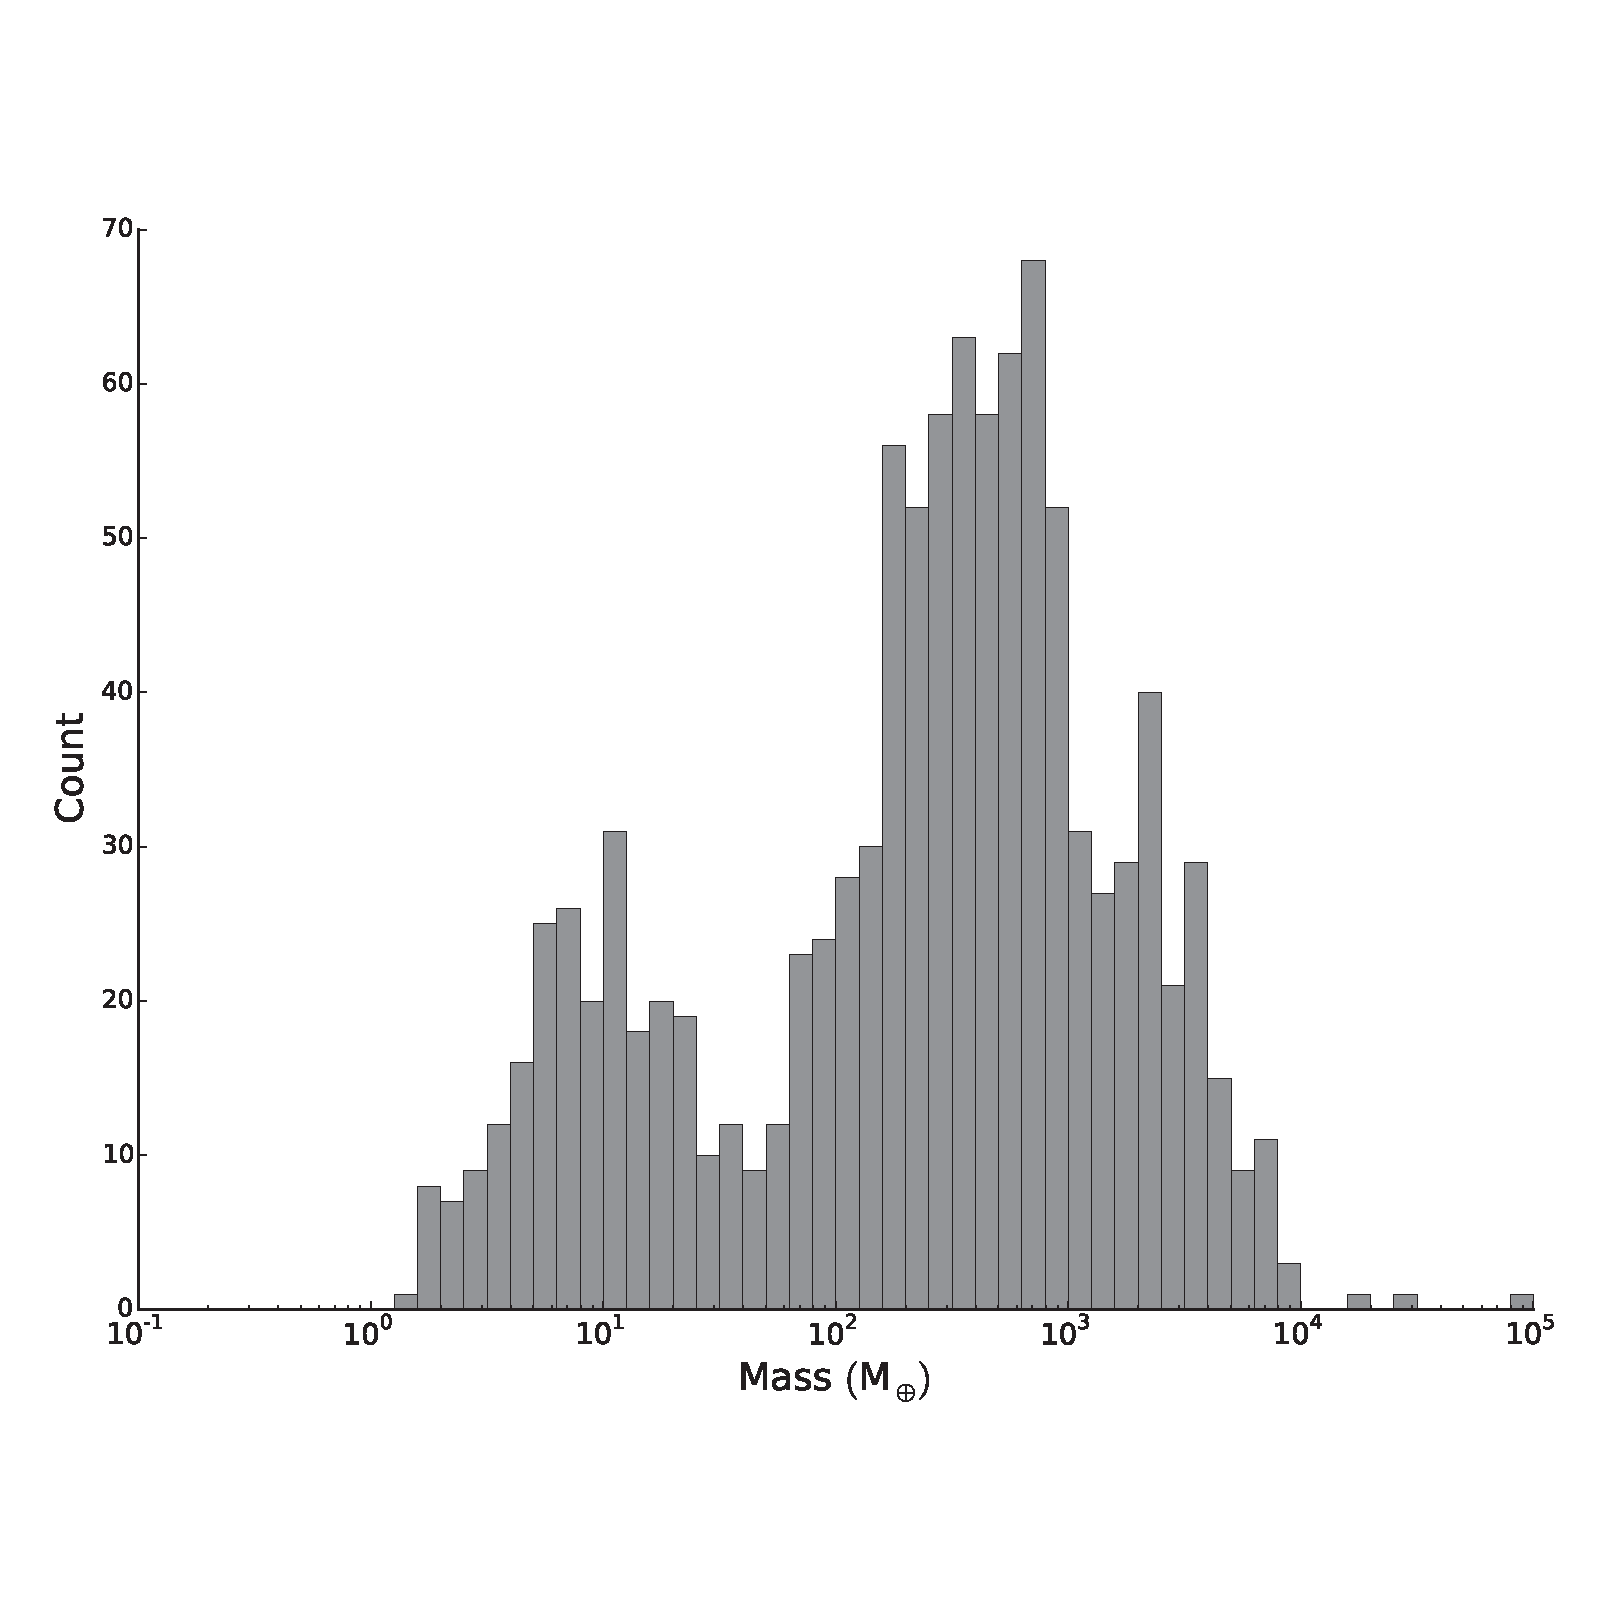
\includegraphics[width=\textwidth]{Chapter3/Figures/ExoplanetsMass.pdf}
        \caption{The distribution of exoplanetary masses for entries in the Open Exoplanet Catalogue \citep{rein2015}}
        \label{fig:exoplanetmass}
\end{figure}

While planets with masses larger than that of Earth seem to be quite common in the sample of observed exoplanets, the mass alone does not imply a composition. In determining composition, the radius of a planet can be a helpful factor as mass and radius combined can give a bulk density. Figure \ref{fig:exoplanetmassradii} shows the mass and radii of 392 planets from the Open Exoplanet Catalogue with measured mass and radii \citep{rein2015}, along with the planets of our solar system, and theoretical mass-radius relations for different bulk compositions. The grey shaded area denotes the region of mass-radius space where super-Earth's are expected to reside.
\begin{figure}
	\centering
        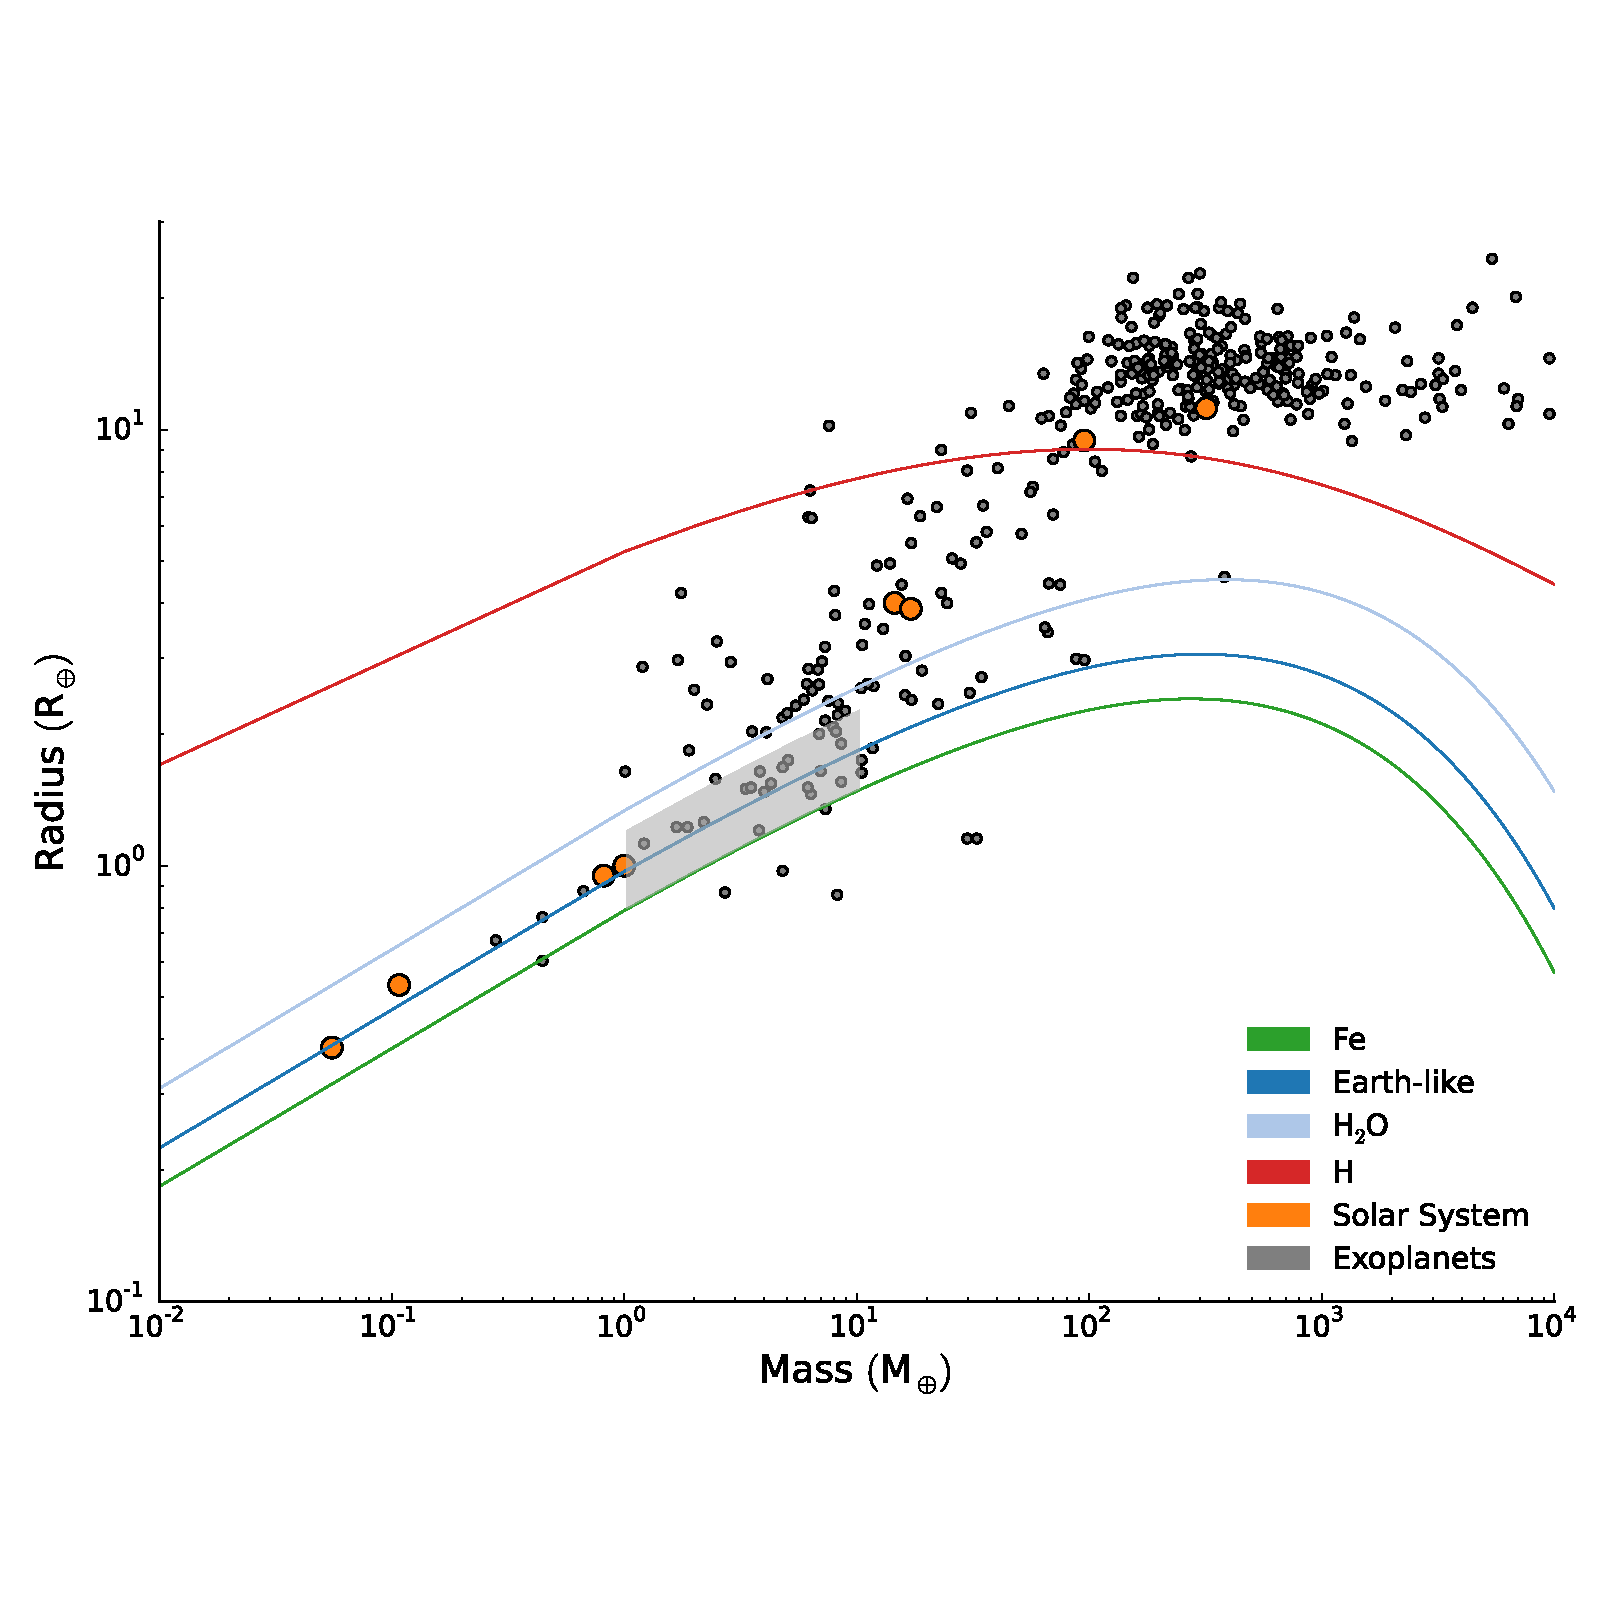
\includegraphics[width=\textwidth]{Chapter3/Figures/ExoplanetsMassRadius.pdf}
        \caption{Planetary radius (in $R_\oplus$) as a function of planetary mass (in $M_\oplus$) for the planets of our solar system (orange circles), the exoplanets in the Open Exoplanet Catalogue with both mass and radius measurements \citep{rein2015} as well as theoretical curves for a pure Fe planet (green), an Earth-like composition ($\textrm{Fe}\left(0.675\right), \textrm{MgSiO}_3(0.325)$, dark blue), a pure $\textrm{H}_{2}\textrm{O}$ planet (light blue) from \citet{seager2007} as well as a pure hydrogen planet (red) from  \citet{zapolsky1969}. The grey shaded region denotes the region of mass-radius space where large terrestrial planets (super-Earth's) should be expected. }
        \label{fig:exoplanetmassradii}
\end{figure}

Figure \ref{fig:exoplanetmassradii} underscores the difficulty of assigning compositions to exoplanets. The lines of constant composition for various combinations of water, ice and rock are very close to each other. When factors such as the uncertainties in both mass and radius, or an atmosphere of unknown mass \citep{adams2008} are added it becomes very difficult to differentiate a large terrestrial planet from a Neptune sized water planet. Nevertheless, the number of planets with mass larger than Earth and radii incompatible with a gaseous composition means that it is likely that super-Earth's are quite common.

\section{Detectability}
Detectability is an important factor in the study of extrasolar planetary magnetic fields. There are two ways that the magnetic field of an extrasolar planet could be detected from Earth. The first occurs when electrons from the stellar wind interact with the dynamo-generated magnetic field from the planet, emitting cyclotron radiation \citep{farrell1999, griessmeier2007, lecacheux1991}. The radiated power associated with this is 
\begin{equation}
P_{rad}\propto B^{0.58} a^{-1.17}
\end{equation}
where $B$ is the magnetic field and $a$ is the planet-star distance. The constant of proportionality is related to the strength of the solar wind \citep{farrell1999}.

The second method by which extrasolar planetary magnetic fields could be detected is through magnetospheric interactions between a close-in planet and its host star. This mechanism was proposed to explain the observations of ``hot spots'' in the chromospheres of some stars, which rotate with the planetary orbit. If a planet with a magnetic field orbits close enough to a star, it is possible the magnetic fields lines may join the two bodies and trap plasma in the closed field lines between them \citep{cohen2009}. The presence of the planetary magnetic field can be detected indirectly through interaction of this plasma with the host star.

Both of these signatures of extrasolar planetary magnetic fields are more easily observable when the magnetic field at the planetary surface is stronger.

\section{Mantle Metallization}
One interesting possibility in super-Earths is the pressure-induced metallization of mantle materials. At high enough pressures, elements which are electrical insulators at ambient or even Earth-mantle pressures will begin to conduct electricity. In order to understand the mechanism behind this, we will briefly discuss the physics of electrical insulators and conductors. More information on the physics of metals and insulators can be found in \citet{ashcroftandmermin}.

\subsection{Band Gaps and Metallization}
If we consider the electronic structure of a solid, we can define two energy ``bands'' that electrons can occupy. The first is the \emph{valence band}, electrons in the valence band are bound to individual atoms and cannot flow between them. The second, at higher electron energy, is the \emph{conduction band}. Electrons in the conduction band are not bound to any atom and can freely flow in response to an applied electric field. Finally, the difference in energy between the lowest energy in the conduction band where the highest energy of the valence band is the \emph{band gap}. In insulators there is a clear separation of energy $E_g$ between the valence band and the conduction band as shown in figure \ref{fig:bandgap}. There are no electrons in the conduction band. In a metal, the band gap is zero, and some electrons occupy the conduction band.
\begin{figure}
	\centering
        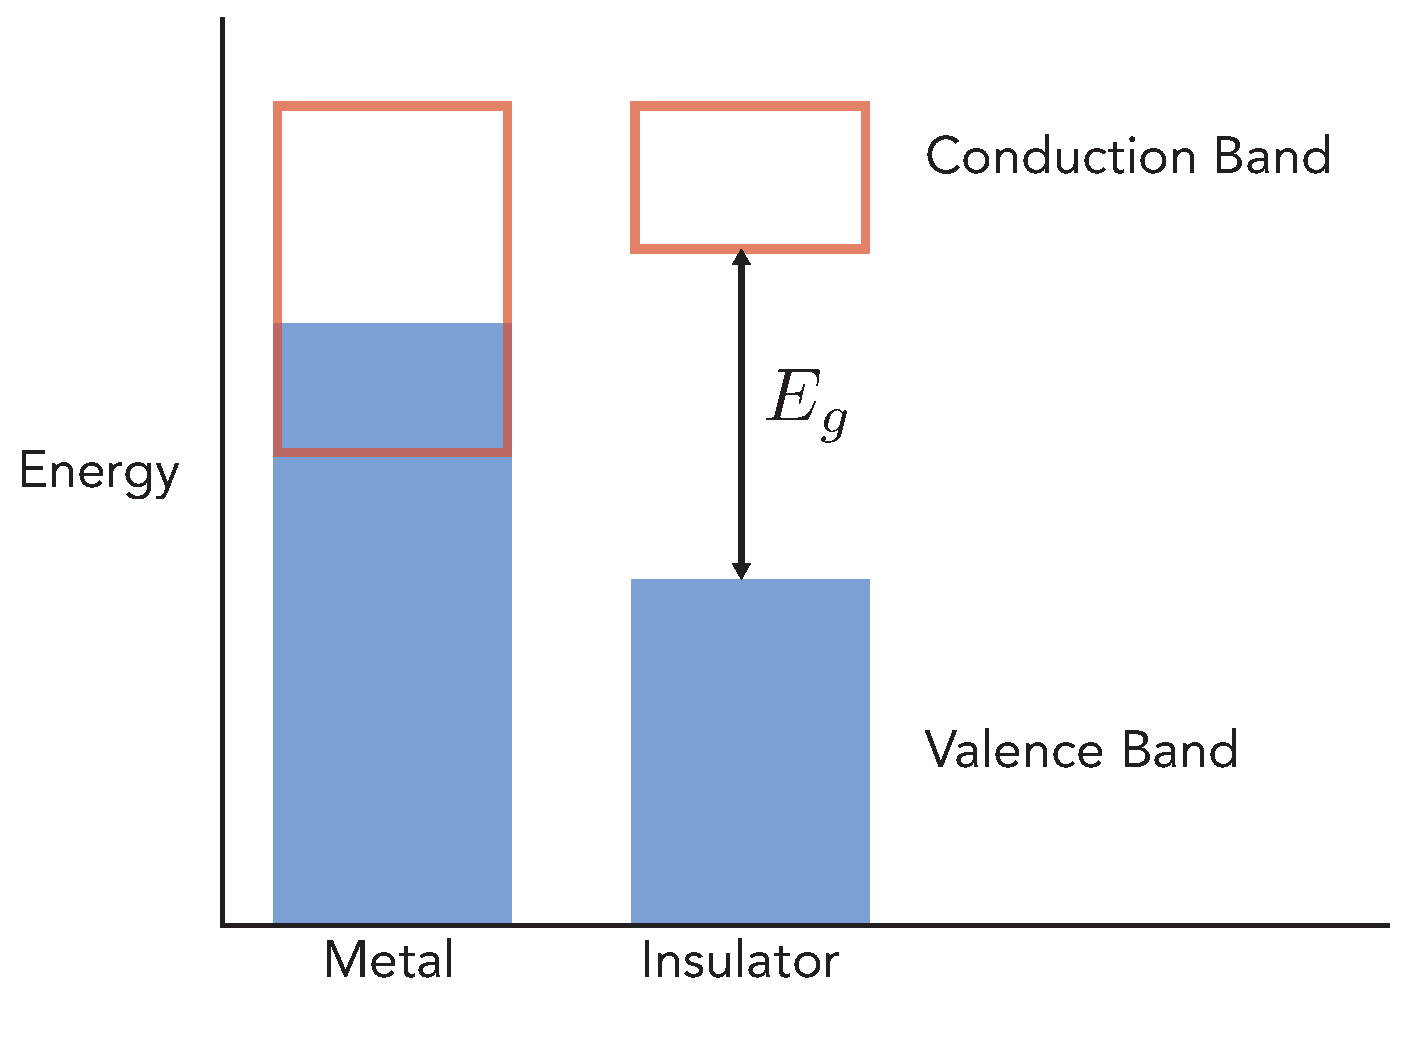
\includegraphics[width=.6\textwidth]{Chapter3/Figures/EnergyGap.eps}
        \caption{A schematic diagram illustrating the difference between the band structure of metals and insulators. Here red indicates the conduction band, and blue indicates the valence band. A filled area indicates that electrons reside at that energy. $E_g$ denotes the band gap.}
        \label{fig:bandgap}
\end{figure}
Importantly, the band gap is pressure dependent, and at high enough pressures it will close, meaning that materials that previously did not conduct electricity become electrical conductors. This process is known as pressure induced metallization.

\subsection{Mantle Metallization in Planets}
In Earth, the mantle is largely electrically insulating, mainly because its main constituent (perovskite) is not expected to metallise until pressures far beyond any which are expected to be found in the deep interiors of even the largest rocky exoplanets \citep{tsuchiya2011}. In exoplanets, the possibility of compositions which differ significantly from Earth could lead to electrically conducting lower mantles in even small rocky exoplanets \citep{ohta2012}. Recent studies have shown that there are several common minerals which should metallise. These include CaSiO$_{3}$ \citep{tsuchiya2011}, FeO \citep{ohta2012}, and Al$_{2}$O$_{3}$ \citep{nellis2010} indicating that lower mantle metallization may be a phenomenon that is common in rocky exoplanets. When mantle materials are metallised a number of their physical properties change significantly. A metallised mantle should have a high thermal conductivity as well as a high electrical conductivity because of the Wiedemann-Franz law, which states that the thermal conductivity is proportional to the electrical conductivity and temperature.

\citet{chan2008} published numerical dynamo simulations with a conducting mantle layer that had  conductivity which varied sinusoidally in latitude and longitude. They found that the addition of this electrically conducting mantle layer could cause a previously steady dynamo to oscillate, and if the conducting mantle layer was thick enough, could stop a dynamo from operating altogether. However, the parameters this study chose were for the benchmark dynamo, an intentionally placid dynamo solution run at unrealistic parameters that is normally used to ensure a numerical dynamo model is working correctly. This raises concerns about its relevance to planetary regimes since the parameters in the benchmark dynamo are much further away from the planetary parameter regime than those used in most planetary studies.

The purposes of these studies was not to model the metallization of the mantle, and so they used lower mantle conductivities than one might expect from a metallic mantle. Furthermore, they concentrated on the effects of heterogeneity in the mantle conductivity. Here we use a numerical dynamo model running at more realistic parameters to study the effect of lower mantle metallization on the dynamos of possible extrasolar terrestrial planets with specific interest in the observable properties of these dynamos.

The study of terrestrial exoplanets, especially terrestrial exoplanetary interiors, remains underconstrained. For a dynamo to exist in these planets, among the most important factors is the state of the mantle. The power  to drive the dynamo of an extrasolar terrestrial planet is controlled by the mantle, so the efficient transfer of heat out of the planet is of great importance. The presence of plate tectonics, and vigorous mantle convection are both efficient ways that planets can drive dynamos in their cores. Currently, mantle convection on these bodies is poorly understood, especially for large exoplanets. The field remains sharply divided \citep{lenardic2012, oneill2007, stein2011, stein2013, valencia2009, vanheck2011} as to the likelihood of plate tectonics, and the viscosity structure \citep{karato2011} of large terrestrial exoplanets. 

The effect of a metallised mantle layer on mantle convection has been studied by \citep{vandenberg2010}. They found that the addition of an electrically conducting layer at the the bottom of the mantle caused the bottom boundary layer to heat, due to the decrease of the local Rayleigh number caused by an increase in the thermal conductivity. This heated lower mantle then becomes buoyant and rises to the upper mantle. This leads to an increased heat flux at the core mantle boundary which could increase the power available to the dynamo, but shorten its lifetime. This would be a secondary effect as the heat flux increase is less than an order of magnitude. There are other, less well constrained properties of extrasolar terrestrial planetary mantles which will have a greater impact on the heat flux from the core than mantle metallization (e.g. radiogenic heating, or the presence of plate tectonics). 

\section{Expected Effects of Mantle Metallization on the Dynamo} 

An electrically conducting mantle should affect the dynamo in two ways. First, any quickly varying components of the magnetic field should be attenuated by the screening effect (see section \ref{sec:screeningderiv}) before they reach the surface, weakening any observed field. Inside the solid mantle layer, the magnetic field obeys a diffusion equation (\ref{eq:nondimmagnetic} with $\mbf{u}=0$), with a diffusivity equal to $\eta=1/(\sigma_{M} \mu_{o})$ where $\sigma_{M}$ is the conductivity of the layer and $\mu_{o}$ is the magnetic permeability of free space. Neglecting the spherical geometry of the core, the magnetic field is attenuated in a solid conducting mantle proportional to $e^{-d\sqrt{\omega/(2 \eta)}}$ where $\omega$ is the frequency of the magnetic field variations at the top of the core and $d$ is the thickness of the conducting mantle. This implies that the thicker the mantle layer, the weaker the observed field. Also, higher multipoles will be preferentially damped due to their more rapid time variation compared to lower multipoles \citep{christensen2004}, while the dipole component of the magnetic field may not be greatly affected.

This screening effect also applies to non-axisymmetric components of the field that are being advected by the background flow at the top of the core. For example, in dynamo simulations, equatorial flux spots are a common occurrence, and typically drift westward \citep{finlay2003}.  From the mantle reference frame these spots are viewed as a time varying magnetic field and hence, they will be screened. In cases where the dynamo generated field is exceptionally steady and axisymmetric, the screening effect may be unimportant as the timescale of field change will be very large.

The second feature we expect when a conducting mantle is added to a dynamo is magnetic shear at the core-mantle boundary (CMB) due to flux freezing in the mantle. The magnetic field should anchor itself in both the solid mantle and the convecting liquid outer core (see \citet{moffatt1978} and section \ref{sec:frozenflux} of this work). Shear should then be created between the solid mantle and the strong zonal flows which are present in planetary cores. Simultaneously, the fluid in the outer core should feel a Lorentz force from the stretching of magnetic field lines anchored in the mantle. While the screening effect is a kinematic process that simply acts on time varying magnetic fields generated by other means, the magnetic coupling effect requires a fully coupled modeling approach.

The thickness of the metallised part of the mantle should have a significant effect on the character of the observable field. We first note that the screening effect and the Lorentz feedback effect scale differently with metallised mantle thickness. Electromagnetic screening becomes more important as the thickness of the metallic mantle layer increases, since the field is attenuated by distance proportional to $e^{-d\sqrt{\omega/(2 \eta)}}$. Conversely, the Lorentz force acting on the fluid by magnetic field anchored in the mantle is nearly independent of mantle thickness. This is evident when examining the equation for the torque ($\Gamma$) on the core by the mantle (adapting \citep{gubbins1987})
\begin{equation}
\Gamma=\frac{r^{2}}{\mu_{o}}\iint\limits_{CMB}B_r\left(\mathbf{r}\mathbf{\mathbf{\times}}\mathbf{B}\right)r^{2} \sin\theta \mathrm{d}\theta \mathrm{d}\phi
\end{equation}
The surface integral is over the core-mantle boundary and does not involve mantle thickness. 

The thickness of the metallised mantle layer in a given exoplanet depends strongly on the size of the planet, the size of the core, and the material which is metallised. For example, FeO should metallise at approximately 55GPa along Earth's geotherm \citep{ohta2012} meaning that a planet significantly smaller than Earth could have an electrically conducting mantle layer as long as it had a large amount of FeO in the mantle. Conversely, CaSiO$_{3}$ is not expected to metallise until pressures of 600GPa, meaning that a conducting mantle layer should form in CaSiO$_{3}$ rich planets with masses greater than 5$M_{Earth}$ \citep{tsuchiya2011}. By varying the composition, planet size, and core size, a conducting mantle layer of nearly any thickness can be achieved. Because of this we avoid fixing a planetary radius or mass, as the arguments here apply equally well to a range of planet sizes. As the surface magnetic field strength is strongly dependent on planetary size and core-mass fraction, we discuss only the properties of the field at the top of the electrically conducting region.
 
\section{Numerical Model}
In this study we use the Kuang-Bloxham numerical dynamo model. We include a solid mantle layer, the electrical conductivity of which can be specified arbitrarily and specify the relative conductivity of the mantle layer with $\sigma_{MC}=\sigma_{M}/\sigma_{C}$ where $\sigma_{M}$ is the conductivity of the conducting mantle layer. All models presented here have $L_{max}=56$, $m_{max}=53$ and the number of grid points in the inner core, outer core, and mantle are $N_{i}=50$, $N_{o}=64$, and $N_{m}=50$ respectively. For numerical reasons we make use of scale-dependent viscosities and diffusivities (hyperdiffusivities, see section \ref{sec:hyperdiffusivity}), we have applied them lightly in this study, using them only for $L>20$ in order to minimise their dynamical effects.

We model a metallised mantle with a spherical shell of uniform conductivity on the outside of the dynamo region. In all models the spherical shell extends from $r_{o}$ to 1.07$r_{o}$. We also make the shell highly conducting, varying $\sigma_{MC}$ from $1/8$ to $1$. As a control, we run a model with a relatively insulating mantle ($\sigma_{MC}=1/400$). A schematic diagram of the model is shown in figure \ref{fig:structure}.
\begin{figure}
\centering
\noindent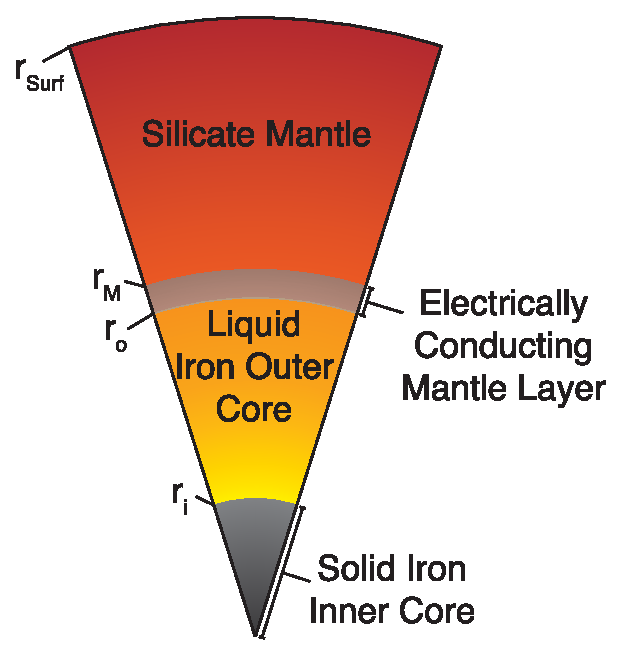
\includegraphics[width=.6\linewidth]{Chapter3/Figures/f1.eps}
\caption{A schematic diagram of the structure of a planet with a conducting mantle layer. Our numerical model solves in the region below $r_{M}$.}
\label{fig:structure}
\end{figure}

The strong rotational influence on convection in planetary cores implies that the solid inner core has a significant effect on the dynamo \citep{heimpel2005, stanleyfluxspot}. Since exoplanets can be found in  different stages of their thermal evolution (depending on their age), we use three different inner core sizes in this study. As a planet ages, the heat lost from the core will cause the solid inner core to grow, so the different cases can be considered proxies for different stages of the life of the dynamo. Here we use $r_{io}=0.35$, $0.5$, and $0.70$. The electrical conductivity of the inner core is the same as the fluid outer core, and the inner core is allowed to rotate independently of the outer core and the mantle in three dimensions in response to viscous and electromagnetic torques exerted on it by the fluid outer core.

\section{Results}
In all cases we find that the addition of an electrically conducting mantle significantly enhances magnetic field generation in our models. The most striking example of this is in the axisymmetric azimuthal ($\phi$) component of the field near the core-mantle boundary (figure \ref{fig:toroidal}).
\begin{figure}
\centering \noindent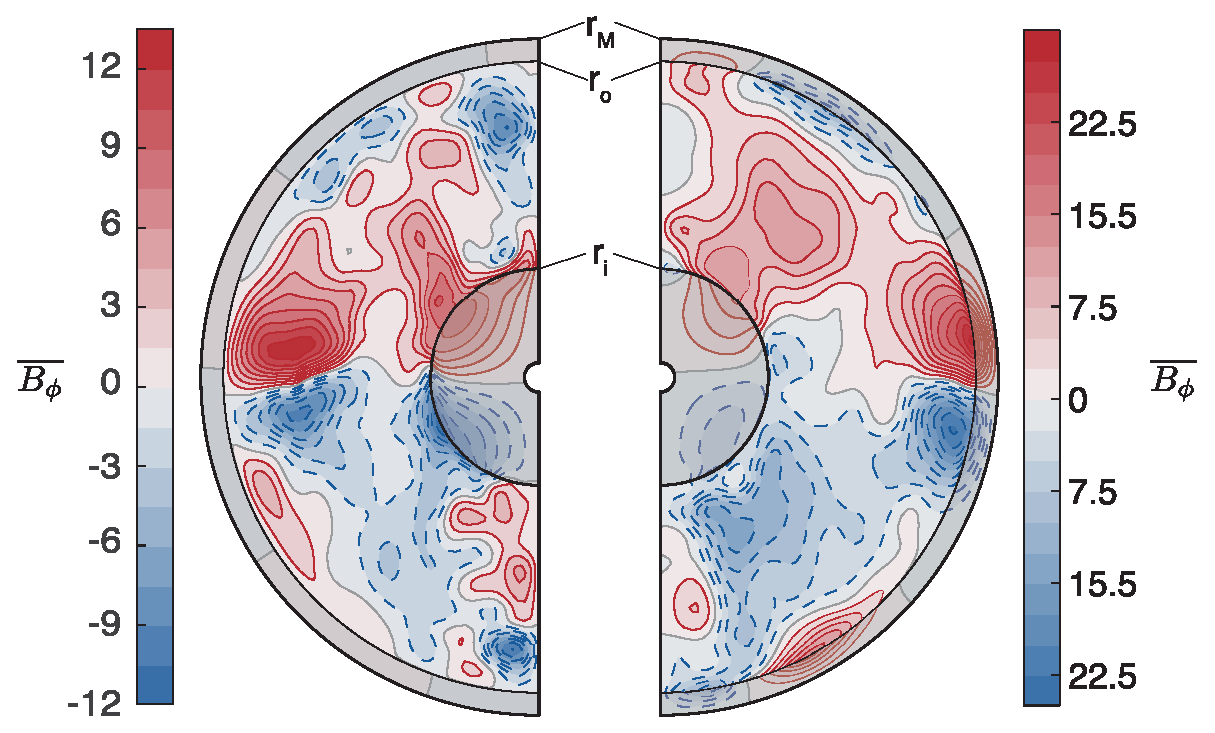
\includegraphics[width=.8\linewidth]{Chapter3/Figures/f2.eps}
\caption{Contours of the axisymmetric azimuthal ($\phi$) component of the magnetic field for an insulating mantle ($\sigma_{MC}=1/400$, left) and for a conducting mantle ($\sigma_{MC}=1$, right) at a single moment in time. The shaded regions indicate the inner core (center) and the conducting mantle layer (outside). Note the difference in scales between the two plots. In these models $r_{io}=0.35$.}
\label{fig:toroidal}
\end{figure}
Here magnetic fields anchored in both the solid, stationary mantle, and the fluid outer core are sheared by the strong zonal flows at the top of the core. This provides a source of magnetic field stretching, which strengthens the magnetic field in the azimuthal direction.

We find that the strength of the poloidal component of the field at the core-mantle boundary is increased as well (figure \ref{fig:cmbenergies35}-\ref{fig:cmbenergies70}).
\begin{figure}
	\centering
        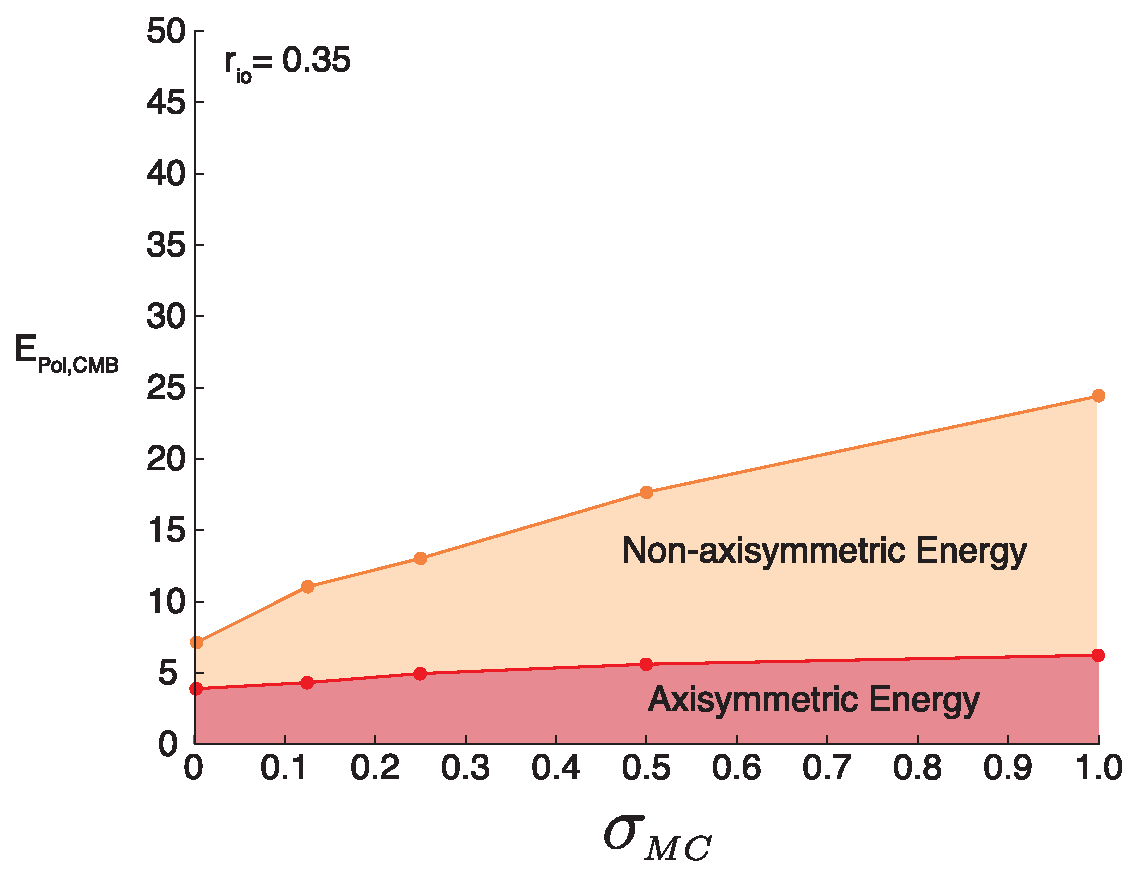
\includegraphics[width=.7\textwidth]{Chapter3/Figures/f3a.eps}
        \caption{The poloidal energies at the core-mantle boundary for $r_{io}=0.35$ separated into non-axisymmetric components (upper) and axisymmetric components (lower). All points are a time average over at least one magnetic diffusion time.}
        \label{fig:cmbenergies35}
\end{figure}
\begin{figure}
	\centering
        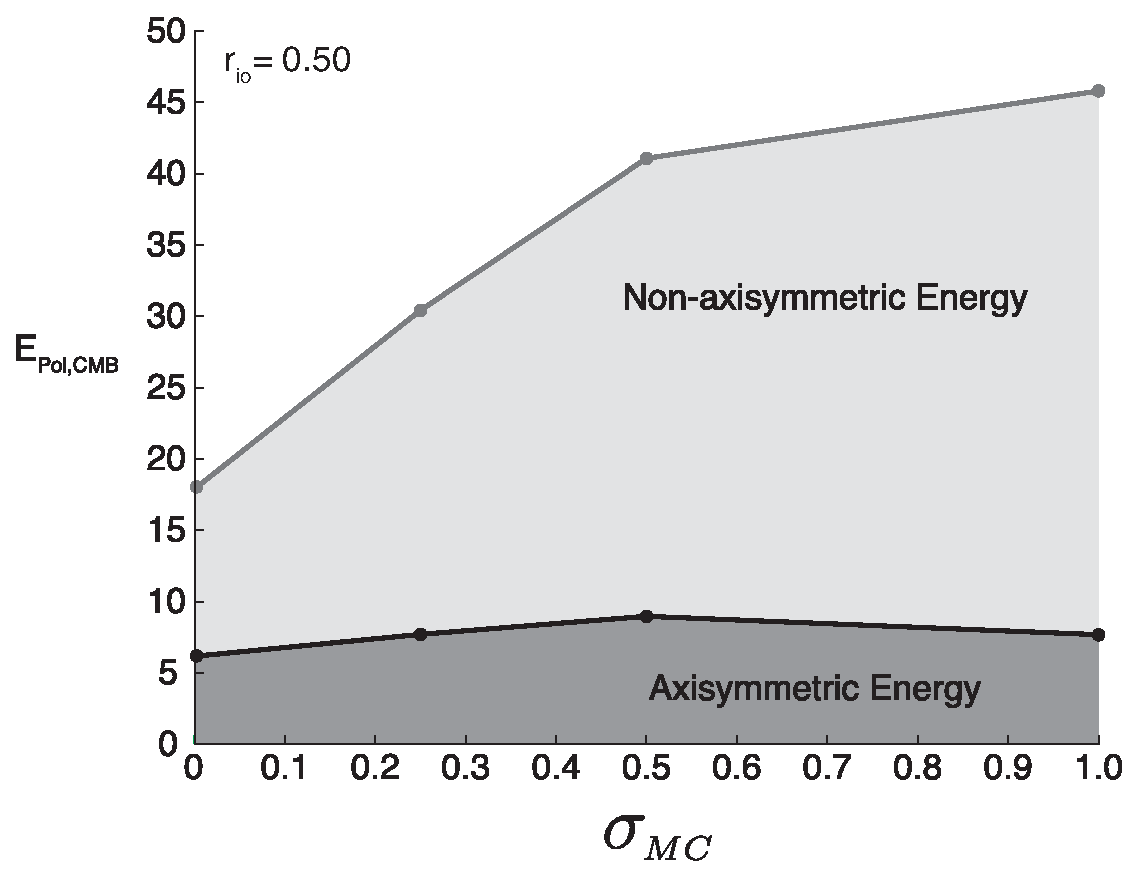
\includegraphics[width=.7\textwidth]{Chapter3/Figures/f3b.eps}
        \caption{The poloidal energies at the core-mantle boundary for $r_{io}=0.50$ separated into non-axisymmetric components (upper) and axisymmetric components (lower). All points are a time average over at least one magnetic diffusion time.}
        \label{fig:cmbenergies50}
\end{figure}
\begin{figure}
	\centering
        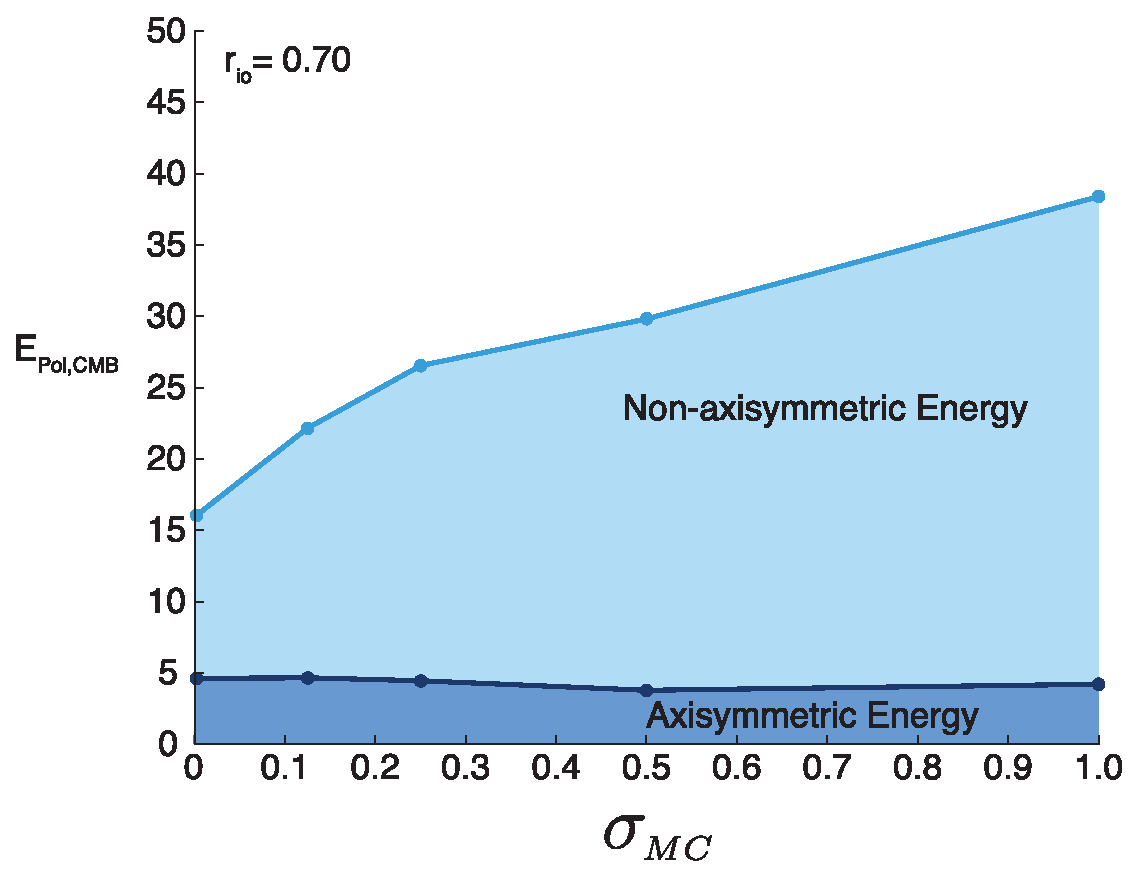
\includegraphics[width=.7\textwidth]{Chapter3/Figures/f3c.eps}
        \caption{The poloidal energies at the core-mantle boundary for $r_{io}=0.70$ separated into non-axisymmetric components (upper) and axisymmetric components (lower). All points are a time average over at least one magnetic diffusion time.}
        \label{fig:cmbenergies70}
\end{figure}

The poloidal component of the field is of special interest as it is the component which is observable from outside the conducting region (the toroidal field requires poloidal currents, which are only present in the conducting region). In our models, the energy in the non-axisymmetric component of the poloidal field increases as the conductivity of the mantle layer increases. In all cases the energy in the axisymmetric component of the poloidal field remains approximately constant.

This preferential increase in the non-axisymmetric component of the field can be explained by noting that the toroidal field at the core-mantle boundary is predominantly axisymmetric, due to the large zonal axisymmetric flows shearing magnetic field there. Given this we can use the Bullard-Gellman formalism (\citet{bullard1954} and Appendix \ref{chap:appendix1}) to show that a dynamo cannot create axisymmetric poloidal energy by any flows acting on axisymmetric toroidal magnetic fields.

In the notation of the Bullard-Gellman formalism, the situation of creating axisymmetric poloidal magnetic field from axisymmetric toroidal magnetic field can be represented as
\begin{equation}
T_{\alpha}^{m_{\alpha}} T_{\beta}^{0} P_{\gamma}^{0} +P_{\alpha}^{m_{\alpha}} T_{\beta}^{0} P_{\gamma}^{0}.
\end{equation}
Recall that $T$ and $P$ represent the toroidal and poloidal fields respectively, $\alpha$ and $m_\alpha$ represent the velocity field spherical harmonic mode, $\beta$ and $m_\beta$ represents the seed magnetic field mode, and $\gamma$ and $m_\gamma$ represents the resultant magnetic field spherical harmonic mode. In this case we include all possible modes of the velocity field, and axisymmetric modes of the seed and magnetic field. 

Evaluating these terms is quite straight forward. The $T_{\alpha}^{m_{\alpha}} T_{\beta}^{0} P_{\gamma}^{0}$ interaction is always identically zero, it merely states that toroidal flows acting on toroidal magnetic fields cannot produce poloidal fields, a well known ``anti-dynamo'' theorem. The $P_{\alpha}^{m_{\alpha}} T_{\beta}^{0} P_{\gamma}^{0}$ interaction requires the selection rules outlined in Appendix \ref{chap:appendix1} to evaluate. Terms of this type depend on an Elsasser integral:
\begin{equation}
L=\oint_{S}Y_{\gamma}^{m_{\gamma}*}\left(\frac{\partial Y_{\alpha}^{m_\alpha}}{\partial \theta}\frac{\partial Y_{\beta}^{m_\beta}}{\partial \phi}-\frac{\partial Y_{\alpha}^{m_\alpha}}{\partial \phi}\frac{\partial Y_{\beta}^{m_\beta}}{\partial \theta}\right)dS.
\end{equation}
This is zero due to a confluence of two of the selection rules for Elsasser integrals. First, in order to be non-zero $m_\alpha\pm m_\beta \pm m_\gamma =0$, implying that $m_\alpha=0$. A second requirement for Elsasser type integral to be non-zero is that either two or none of the harmonics has a $\cos\left(m\phi\right)$ term ($m=0$ is a cosine term here). Since all three of our harmonics have $m=0$ we have three cosine terms, meaning the $P_{\alpha}^{m_{\alpha}} T_{\beta}^{0} P_{\gamma}^{0}$ is always zero. Hence, we should expect that the axisymmetric poloidal field should not increase due to an increase in the axisymmetric toroidal field caused by a conducting mantle layer. This application of the selection rules only applies to cases where $m=0$ for all three modes. It is possible to create non-axisymmetric poloidal fields via non-axisymmetric velocities acting on axisymmetric toroidal magnetic fields, so an increase in the strength of the axisymmetric toroidal magnetic field should imply an increase in the strength of the non-axisymmetric poloidal magnetic field. 

The axisymmetry of a dynamo is an important factor in the potential observability of extrasolar terrestrial planetary magnetic fields. For the magnetic field to reach the exterior of the planet where it can be observed, it must first be screened through a conducting lower mantle. As  discussed earlier, non-axisymmetric fields are screened more efficiently than axisymmetric fields. This becomes apparent if we plot the poloidal magnetic energies above the conducting layer (figure \ref{fig:ddppoloidaltotal}).
\begin{figure}
\noindent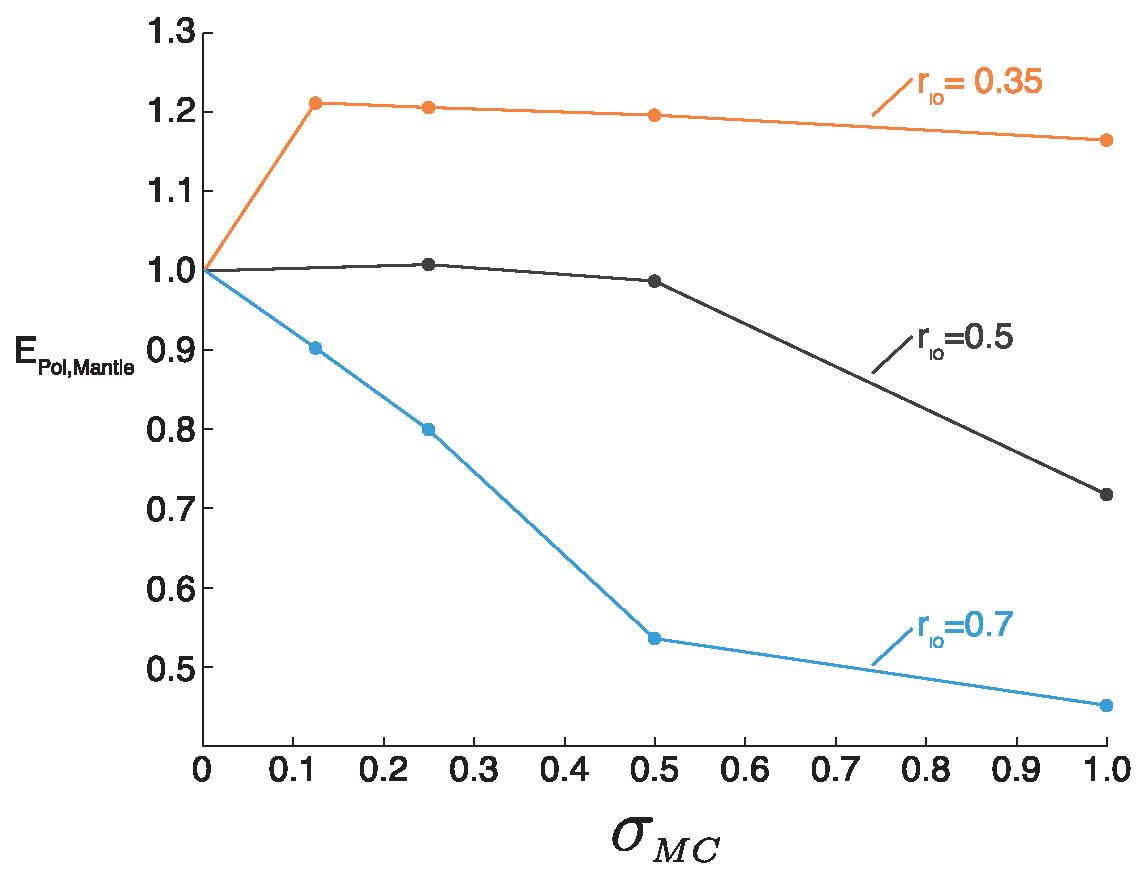
\includegraphics[width=.7\linewidth]{Chapter3/Figures/f4.eps}
\centering
\caption{Total poloidal energy at the top of the conducting layer ($r_{M}$) as a function of mantle conductivity. All points are a time average over at least one magnetic diffusion time and have been normalised to the insulating mantle case.}
\label{fig:ddppoloidaltotal}
\end{figure}
We see that depending on the inner core size, the observable field is either only marginally stronger, or much weaker than the field in a model without a conducting mantle layer.

As $r_{io}$ increases there is a marked decrease in poloidal field strength at the top of the conducting layer relative to the insulating case (figure \ref{fig:ddppoloidaltotal}). When considered with figures \ref{fig:cmbenergies35}-\ref{fig:cmbenergies70}, the reason for this becomes clear. As the liquid outer core becomes thinner the dynamo becomes less axisymmetric at the top of the dynamo region and the characteristic timescale of variation becomes shorter \citep{aubert2009}. Both of these effects cause the field to be weakened by the screening effect of the conducting layer. This means thinner shells are more susceptible to the screening effect discussed earlier. The increase in non-axisymmetry with increasing $r_{io}$ has been observed previously in studies which modelled the evolution of Earth's dynamo through time \citep{aubert2009, roberts2001}.

\section{Conclusions}

We have used a numerical planetary dynamo model to investigate the effect of the metallization of silicate mantles on the observable magnetic fields of super-Earths. We have carried out models for three different inner core sizes to simulate these planets at different stages in their thermal evolution. In all cases we find that the strength of the internal magnetic field increases substantially, owing to the magnetic shear provided at the core-mantle boundary by the conducting mantle. We also find that the addition of a conducting mantle makes the field significantly less axisymmetric at the top of the dynamo region. After being screened through the conducting mantle layer we find that the observable field shows either a modest increase in field strength (at $r_{io}=0.35$) or a significant decrease in field strength (at $r_{io}=0.7$). The results of this work are published in \citet{vilim2013}

As we have used a thin conducting layer in these models (compared to the range that is possible for terrestrial exoplanets), we expect that in larger planets, the screening effect would be even stronger than we observe here. This means that any planets with a metallised mantle should have surface fields which have been significantly weakened by a combination of the non-axisymmetrisation of the dynamo, and the screening effect of the mantle. We therefore expect that the metallization of silicates should make the detection of dynamo-generated magnetic fields from super-Earth's more difficult than previously anticipated \citep{driscoll2011}.










%!TEX root = ../thesis.tex
\chapter{Iron Snow Zones as a Cause for Mercury's Weak Observed Magnetic Field}
\label{chap:doublesnowstates}
\chaptermark{Iron Snow Zones in Mercury}
\section{Introduction}
The planet Mercury is in many ways unique in our solar system. It is the smallest planet, which orbits fastest, and closest to the sun. It is also unique in the solar system by being the only planet which has any kind of tidal locking to the sun. Mercury is in a 3:2 spin-orbit resonance, meaning that it rotates three times for every two orbits. It is also the planet with the greatest orbital eccentricity ($e=0.2056$, compared to the Earth's $e=0.0167$) and the lowest obliquity ($\epsilon=1/30^\circ$ compared to Earth's present obliquity of $\epsilon=23.4^\circ$). This means the same ``seasons'' on Mercury occur in the north and south hemisphere at the same time and are primarily determined by the distance the planet is from the sun, rather than the obliquity.

\subsection{Mercury's Internal Structure}
Understanding the structure and processes at play within Mercury is crucial to understanding how magnetic field generation happens within the planet. The crudest way of examining Mercury's internal structure is to discuss the mean uncompressed density of the planet, which, at 5.4 $\textrm{g}/\textrm{cm}^3$ is the largest of any of the terrestrial planets. This means that the composition of Mercury must be much more iron-rich than any other planet in the solar system, indicating a large iron core may be present. 

Observations of longitudinal librations by \citet{margot2007} provided two key insights into the interior structure of Mercury. First, they observed a large amplitude longitudinal libration which indicates that the mantle and the core are librating separately. This large amplitude libration implies a moment of inertia which is much smaller than would be observed for Mercury if the whole planet librated together. This means that a liquid layer must be present between the surface and the deep interior of the planet, assumed to be a liquid iron outer core. Second, they confirmed that Mercury is in a Cassini state 1, where spin axis and orbit normal point in the same direction and are both normal to the orbital plane. When these observations are synthesised with the degree two gravitational moments from the recent MESSENGER (MErcury Surface, Space ENvironment, GEochemistry, and Ranging) mission \citep{smith2012}, the polar moment of inertia ($C$) and the moment of inertia of the librating solid shell ($C_M$, presumed to be a solid mantle and crust) can be deduced \citep{peale1969}. This work will be discussed in greater detail in chapter \ref{chap:floatationlayers}.

The moment of inertia measurements by \citet{margot2012} were used by \citet{hauck2013}, along assumptions about the composition of Mercury, to deduce more complicated information about the internal structure of Mercury. They found that the size of Mercury's core is likely $2020 \pm 30\textrm{km}$. They also found that the mean compressed density of the solid region above the core is $3380\pm200 \textrm{kg} \textrm{m}^{-3}$ while the density below the boundary is $6980\pm280 \textrm{kg} \textrm{m}^{-3}$.

\citet{rivoldini2013} took a different approach to modelling Mercury's interior which used the libration amplitude of \citet{margot2012} directly, rather than $C_M$ and allowed for gravitational coupling between a possible inner core. They found a core size of $2004 \pm 39 \textrm{km}$ and a core density of  $7233\pm267 \textrm{kg} \textrm{m}^{-3}$, however they felt that the mantle density was too unconstrained to offer an estimate.

\subsection{Mercury's Magnetic Field} 
Before spacecraft began visiting Mercury it was thought that Mercury's core would be completely solid. Small bodies have a higher surface area to volume ratio than large bodies which results in shorter cooling times \citep{siegfried1974} . Since a solid core does not possess the fluid motions necessary to make an active planetary dynamo, it was thought that any magnetic fields observed from Mercury would be remnant fields frozen into the crustal rocks. In 1974 Mariner 10 flew by the planet three times, making magnetic field observations on two of those flyby's. Data from these flyby's revealed the presence of a weak, predominantly dipolar magnetic field \citep{nessmariner10}.

This weak magnetic field proved to be quite difficult to explain using the tools available to planetary scientists at the time for two reasons. First, the strength of the magnetic field was much greater than could reasonably be frozen into crustal rocks unless the magnetic mineral was very highly magnetised and also very shallow. Secondly, \citet{runcorn1976} showed that a homogenous spherical shell cannot be internally magnetised to display a dipolar field. Although the existence of crustal inhomogeneities relaxes the constraints set by Runcorn's theorem  \citep{Aharonson2004}, it remained difficult to explain Mercury's magnetic field using crustal magnetism.

Since Mercury's core was thought to be solidified, several proposals were put forward to explain the observed magnetic field using mechanisms besides an active core dynamo. Eventually the discovery of an active dynamo in Ganymede \citep{kivelson1996} (showing that small body dynamos were possible), and the discovery of a liquid layer in Mercury's core by Earth-based librational measurements \citep{margot2007,margot2012} established that an active dynamo is the likely source of Mercury's magnetic field.

An active dynamo in Mercury presents a new set of questions to planetary scientists. While the measured magnetic fields were too strong to be easily explained by crustal remnant magnetism, they are much weaker than can easily be explained by a standard core dynamo. The MESSENGER spacecraft has made measurements of Mercury's magnetic field that agree with those made by Mariner 10 and have placed the $\mathrm{g}_1^0$ Gauss coefficient at $190\pm 14$ nT and the dipole tilt at less than $0.8^{\circ}$ from the rotation axis \citep{anderson2012}. Magnetic field measurements by MESSENGER have also revealed the presence of higher multipoles in Mercury's magnetic field, most importantly they have constrained the axial quadrupole Gauss coefficient ($\mathrm{g}_{2}^0$) to be $74\pm4$nT. This has the effect of moving the magnetic equator northward by approximately 400km or 20\% of the planets radius \citep{anderson2012}. The surface radial magnetic field including all known Gauss coefficients is shown in figure \ref{fig:Mercurybr}.
\begin{figure}
	\centering
	\noindent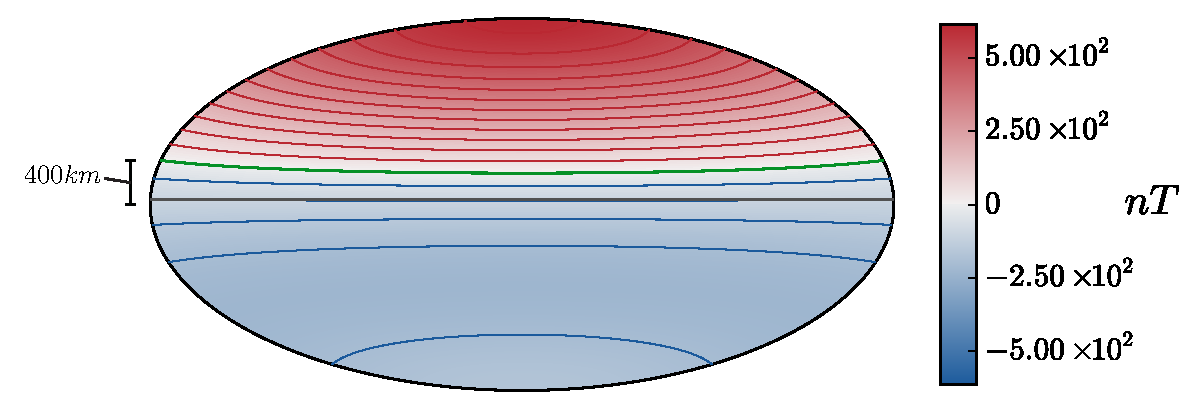
\includegraphics[width=\linewidth]{Chapter4/figures/Mercury_br.pdf}
	\caption{Mercury's surface radial magnetic field for all known Gauss coefficients ($\mathrm{g}_1^0$ and $\mathrm{g}_2^0$). The green horizontal line denotes the magnetic equator while the black horizontal line denotes the planetary equator.}
	\label{fig:Mercurybr}
\end{figure}

\subsection{Dynamo Explanations for Mercury's Field}
One way a dynamo could produce a weak surface field is through a non-Earth-like field partitioning. There are several methods through which the magnetic field strength of Mercury can be estimated. One method assumes that to first order, the Coriolis and Lorentz forces will balance in the core; this is known as magnetostrophic balance (see section \ref{subsec:magnetostrophic}). Magnetostrophic balance implies an estimated magnetic field strength of $B=\sqrt{2\Omega\eta\rho\mu_{o}}$ where $\Omega$ is the rotation rate of the planet, $\eta$ is the magnetic diffusivity, $\rho$ is the density, and $\mu_o$ is the magnetic permeability of free space. If reasonable values are used for this estimate (Table \ref{tab:runs}), then a magnetic field strength within the core of $10^{5}-10^{7}$nT is obtained.

This estimation alone does not necessarily conflict with the observations of Mercury's field, since it predicts the magnetic field within the core while observations are made by spacecraft in the potential region outside the planet. The total magnetic field can be decomposed into poloidal $(\mathbf{B}_{P})$ and toroidal $(\mathbf{B}_{T})$ field components with the toroidal-poloidal  decomposition (see section \ref{sec:representations}):
\begin{equation}
\mathbf{B}=\mathbf{B}_{T}+\mathbf{B}_{P}=\nabla\times\left(T\hat{r}\right)+\nabla\times\nabla\times\left(P\hat{r}\right)
\end{equation}
where $T$ and $P$ are the toroidal and poloidal scalars, and $\hat{r}$ is the unit vector in the radial direction. Only the poloidal field has a radial component, and is therefore the only component that is observable from outside the core. If the Mercurian dynamo is similar to the Earth's in character, then there should be a similar partitioning between toroidal and poloidal field components. If the dipole moment at the core mantle boundary (CMB) is taken to be representative of the poloidal component, then it can be shown that for Mercury, $B_{dip}/B_{T}\approx10^{-2}-10^{-4}$, whereas for Earth $B_{dip}/B_{T} \approx 10^{-1}$  \citep{stevenson87}. The conclusion from this analysis is that if Mercury exists in the strong field regime (i.e. that the dynamo is in magnetostrophic balance), then a distinctly non-Earth-like field partitioning should be expected. Although this analysis is rather simplistic, it can be repeated using thermodynamic arguments instead of force balance arguments \citep{schubertandross88,stevenson87} resulting in similar total field strengths.

Several studies \citep{stanleyandbloxham2005,heimpelandaurnou2005,christensen06,takahashi06} have produced dynamo models with dipole moments of the same order as the observed Mercurian field through exotic field partitioning. This is accomplished either by making the inner core boundary (ICB) to core mantle boundary (CMB) radii ratios ($r_{io}$) very small ($0.15$ in \citet{heimpelandaurnou2005} or very large ($0.8$ in \citet{stanleyandbloxham2005}).

Another possibility is that Mercury's dynamo is not dipole dominated. Different scalings by \citet{OlsonandChristensen2006} have found that the dynamo should be in a state which produces a strong, multipolar dynamo. \citet{christensen06} used evidence that the temperature gradient across the core mantle boundary may be subadiabatic to justify a stably stratified layer occupying the top portion of Mercury's core. He argues from local Rossby number considerations (see section \ref{sec:rol}) that Mercury's dynamo should be multipolar, and that the surrounding stable shell preferentially attenuates higher multipoles, leaving a slowly varying, weak dipolar field. A subsequent study by \citet{manglik2010} showed that a growing inner core would release enough light element to disrupt any thermal stable stratification. They found this would lead to a strong, non-dipolar magnetic field. This means that a mechanism besides a subadiabatic heat flux is required to maintain the stable stratification if this mechanism is to work.

The final way that a weak surface field has been produced involves appealing to interactions with the solar wind. \citet{glassmaier2007} showed that Chapman-Ferraro currents induced by the interaction of Mercury's magnetosphere with the solar wind could produce magnetic fields in its core which  weaken the dynamo. Using a kinematic model based on work by \citet{levy1979}, they showed that this ``feedback dynamo'' could account for the weak observed magnetic field of Mercury. The initial temporal evolution of this model was further investigated by \citet{heyner2010} and it was modelled in a full, nonlinear dynamo model by \citet{heyner2011}.

All of these studies were done before the $g_2^0$ Gauss coefficient was measured by MESSENGER and none of them predicted $g_2^0$ accurately. Since the $g_2^0$ was measured, \citet{cao2014} published a study that used volumetric buoyancy and inhomogeneous heat flux thermal boundary conditions to shift the magnetic equator, however this study did not reproduce Mercury's weak observed magnetic field.

Because no model simultaneously reproduces both the weak field strength, and the equatorial displacement of the magnetic field (i.e. the correct $g_2^0$) we can conclude that the cause of Mercury's magnetic field remains an open question in planetary science.

\subsection{The State of Mercury's Core}

All dynamo explanations require that the core of Mercury remain at least partially liquid to the present day, something that is quite difficult to do with a small planet with a core composed purely of iron. The detection of a dipolar magnetic field by Mariner 10 implied the existence of a liquid region due to the dynamo hypothesis, and observational evidence of longitudinal librations \citep{margot2007, margot2012} strongly suggests the existence of a liquid layer in Mercury. 

Although there is likely a liquid region in Mercury's core, the size of the liquid outer core is not well constrained. Most studies attribute the existence of a liquid outer core to the presence of a light element, such as sulphur, which would depress the freezing point of iron. Like the size of the inner core, the sulphur content of the outer core is not well constrained. Thermal evolution models \citep{schubertandross88} have shown that while it is difficult to prevent the core of a planet as small as Mercury from freezing, if the core contains some sulphur it is possible to keep the core partially liquid to the present day. If other effects such as temperature- and pressure-dependant rheologies \citep{conzelmann99,hauck04,brueur07} or tidal dissipation \citep{schubertandross88} are accounted for, almost any inner core to outer core radius ratio can be produced. As a result, the size of the inner core remains rather unconstrained. 

In a recent study, \citet{dumberry2015} used the moment of inertia and librational amplitude to extract further information about the state of Mercury's core. They find that the largest inner core compatible with these observations at the $1\sigma$ level is $1325 \pm 250\textrm{km}$ or $r_{io}=0.6\pm 0.1$.

Work by \citet{chenetal2008} has shown through a combination of new experiments on the non-ideal behavior of iron sulphur alloys at moderate pressures and existing data for higher-pressure melting of these alloys \citep{stewart07}, that Mercury may have a very different core crystallization regime than any other body, save possibly Ganymede \citep{hauck06}. The result is the formation of an iron precipitate at different radii throughout the core, the exact location and number of which is dependent on sulphur content. Once an iron precipitate forms, it begins to sink, while the residual, more sulphur-rich liquid rises. The generation of iron ``snow'' acts as a source of compositional convection, affecting fluid motions and therefore the dynamo.

If the liquid portion of the core contains between approximately 7 wt\% and 8 wt\% sulphur, an iron precipitate forms near the CMB and falls towards the inner core, this is referred to as a shallow snow state. For states with between approximately 8 wt\% and 10 wt\% sulphur, a snow layer at approximately 23 GPa and deeper will form as well (a double snow state). In this case we would expect two sources of compositional convection, one from the dense iron precipitate falling towards the planetary center, and another from the liberated sulphur rising towards the CMB. A schematic of the ``double snow state'' scenario is shown in figure \ref{fig:setup}(a). Finally, if the liquid outer core contains more than 10 wt\% sulphur, the snow zone at the CMB disappears, and only the deeper snow zone remains (a deep snow state). Although other light elements (such as O, Si, C, N, or H) can depress the freezing point of liquid iron, and could be present in Mercury's core, the iron-sulphur system is the best characterised. At this point there is no evidence to suggest snow zones occur in systems with different constituents. 

Here we use a numerical dynamo model to examine whether the effects of snow zones on Mercury's dynamo could explain its weak magnetic field. In the following sections we discuss a method of incorporating snow zones into the models, and the characteristics of the resulting fields. In this study we focus on double and deep snow states, since previous work demonstrated that shallow snow state models produce Earth-like dipole intensities when in magnetostrophic balance \citep{stanleyandmohammadi}.

We also exclude double and deep snow states in which the deep snow zone extends all the way to the ICB. In this scenario, motions in the lower region of the dynamo would be very small scale, since this region would be in a diffusive staircase convection regime. A state similar to this has already been explored by \citet{stanleyandbloxham2006} in the context of Uranus and Neptune. They found that strong, multipolar fields result, which do not match the observed field of Mercury.

\section{Modelling a Snow Zone}
To model a snow zone in a numerical dynamo model, we first observe that as iron solidifies it injects buoyancy into the core. For example, in Earth pure iron solidifies at the inner core boundary and the residual light element is released into the fluid. This light element is now lighter than the bulk fluid and is therefore buoyant. We can use similar reasoning to add a snow zone to a numerical dynamo model. There are two effects which need to be taken into account when implementing a snow zone. First, the negative buoyancy representing the sinking iron, and secondly the positive buoyancy due to the remaining sulphur rich fluid.

To incorporate both effects, we model a single snow zone as two thin shells: a source of co-density directly above a sink of co-density. The background co-density profile $C_{0}\left(r\right)$ is then determined by solving equation (\ref{eq:dimensionalbgcodensity}) with the given $Q\left(r\right)$. We find that a snow layer can be represented as a stably stratified layer in the slope of the background co-density profile. For the sake of simplicity, we make it a layer of constant $d C_{0}\left(r\right)/dr$ (figure \ref{fig:setup}(b)). It should be noted that this representation of a snow layer does not attempt to capture the specific dynamics of iron snow, but rather their net effects. Our model of a snow layer is quite crude, it will be the goal of future studies to make it more realistic.
\begin{figure}
	\centering
	\noindent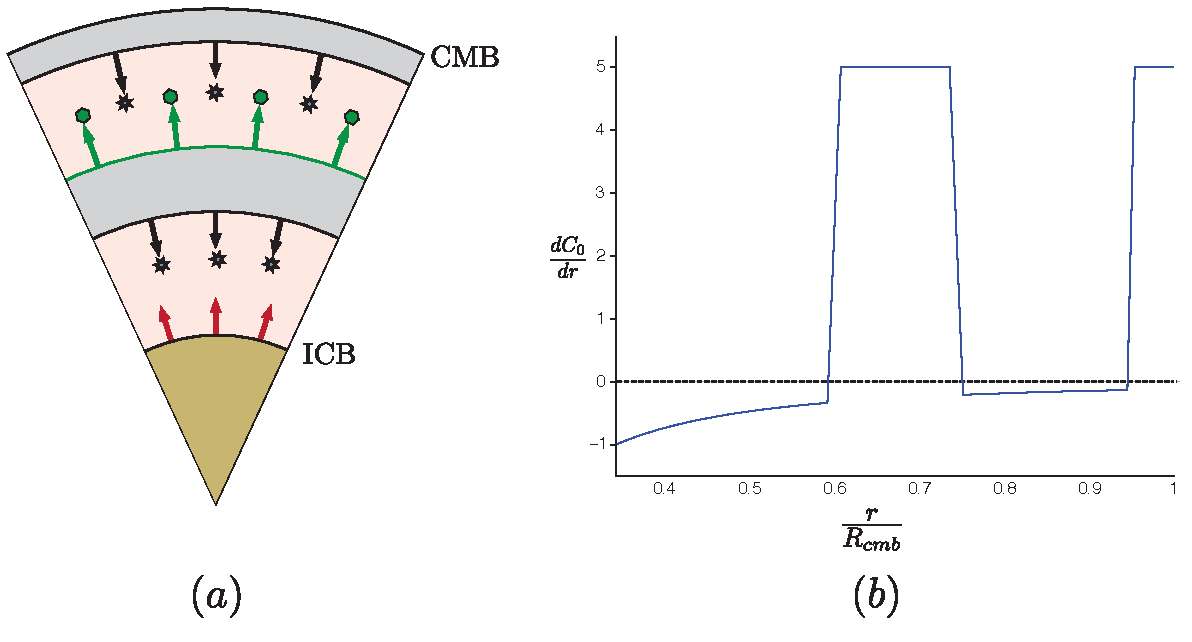
\includegraphics[width=40pc]{Chapter4/figures/setup.pdf}
	\caption{a) A schematic diagram of a core in a double snow state, the snow layers are indicated by the grey bands. The compositional effects are indicated by arrows, sulphur driven effects are indicated in green hexagons, while iron driven effects are in black stars, thermally driven effects are indicated by red arrows. b) The slope of the background co-density profile for a double snow state. Areas of positive $dC_{0}/dr$ indicate stably stratified regions, or snow zones. The dashed line indicates the neutral buoyancy profile ($dC_{0}/dr=0$).}
	\label{fig:setup}
\end{figure}

Our representation of a snow layer as a stably stratified region makes physical sense if we consider the path of an individual parcel buoyant at the ICB. This parcel will begin to rise, and will remain buoyant and rise until it reaches the base of the deep snow layer where it begins to solidify, expelling any light element mixed in with it, and losing its buoyancy. It then descends back into the lower layer. In this regard, the base of the snow layer is both a stably stratified layer (reducing the buoyancy of the rising parcel) and a source of compositional buoyancy in the lower layer (releasing iron which is denser than its surroundings). Similarly, the sulphur released in the deep snow layer is more buoyant than the fluid immediately above the deep snow layer and acts as a source of buoyancy for the upper region. For simplicity we do not consider the energy associated with latent heat release and consumption. Since compositionally driven convection is thermodynamically more efficient than the thermal component of convection, this is likely a reasonable first-order assumption.

As a result of the large uncertainties associated with many of the quantities in planetary cores, the strength of the stable stratification due to the snow layer is unknown. In our models, we assume that the compositional sources of buoyancy resulting from iron snow zones are the primary driver of convection within Mercury, thus the stably stratified layer would be strongly stratified relative to the co-density flux at the inner core boundary. We found that our results remained largely the same so long as the snow layers are the primary driver of convection in our models.

The thickness of the snow layer is another quantity which can vary widely depending on the sulphur content and on the adiabat \citep{chenetal2008}. We have chosen a deep snow layer thickness of $0.13 R_{CMB}$. This falls within the range of values predicted from the data in \citet{chenetal2008}. Investigating the effect of snow layer thickness on the dynamo will be the goal of future work in this field. In this study, the deep snow zone extends from $0.61 R_{CMB}$ to $0.74 R_{CMB}$, where $R_{CMB}$ is assumed to be $0.75 R_{\textrm{M}}$.

In all cases the maximum spherical harmonic degree is 33 and the maximum order is 21. In the radial direction we used 119 grid points, 36 of which were in the inner core, 64 of which were in the fluid region and 19 of which were in the thin, weakly conducting mantle layer.

The models presented here used hyperdiffusivities (equations \ref{eq:hyperdiffseta}-\ref{eq:hyperdiffsnu}) with $\hat{\eta}=\hat{\kappa}=0.06$ and $\hat{\nu}=0.05$. Preliminary results on higher resolution runs ($L_{max}=90$, $m_{max}=85$, $n_{r}=95$) show that the resolution used in our models is not an issue when hyperdiffusivities are implemented ($l_{o}=0$).

In all models presented here, constant co-density flux boundary conditions were applied to both the inner core boundary and the core mantle boundary. When constant co-density boundary conditions were used instead, there was no significant qualitative differences in the models. 

In all cases we kept the inner core to outer core radius ratio ($r_{io}$) fixed at $12/35$. This is consistent with the predictions of \citet{hauck04} when they used sulphur contents high enough to develop double and deep snow states. In our study we chose a moderately low Ekman number of $2\times10^{-5}$ to reduce the effects of viscosity in our model. Although this is much larger than the Ekman number expected for Mercury (on the order of $10^{-13}$), at present it is numerically infeasible to work at such low Ekman numbers. Stress free boundary conditions are also used to minimise Ekman boundary layer effects, which would be far too large if we chose to use no-slip boundary conditions. We used finite electrically conducting boundary conditions on the magnetic field. We also set our magnetic Rossby number to be $2\times10^{-5}$, and set both of our Prandtl numbers to 1. Only the modified Rayleigh number  and initial conditions were varied between the models. In these models the critical Rayleigh number is approximately $700$.

\section{Results}
\subsection{Dipole Moment}

\citet{chenetal2008} outline three basic configurations for iron snow zones in Mercury's core: a single snow zone at the CMB (shallow snow state), a snow zone at the CMB along with one midway through the core (double snow state), and a single snow zone midway through the core (deep snow state). We found that only models with a deep snow layer (double and deep snow states)  which does not extend to the ICB successfully produced a weak dipolar field.  The results for the simulations of interest are summarised in Table \ref{tab:runs}. In all cases the dipole moment was relatively stable. Although several dipole reversals did occur, the field usually returned to a stable configuration akin to its pre-reversal state, though of opposite polarity. In most models the dipole tilt is quite small, for a non-reversing segment of model 2, the dipole tilt averaged over approximately half a magnetic diffusion time was $6^{\circ}$ away from the rotation axis.
\begin{table*}
\centering
%\begin{tabular}{c c  l  r @{.} l   r @{.} l   r @{.} l   r @{.} l   r @{.} l   r @{.} l   r @{.} l r @{.} l r @{.} l  }
%Model & Ra & Model Type & \multicolumn{6}{c}{Dipole Moment} & \multicolumn{6}{c}{$B_{dip}/B_{T}\times10^{-3}$} & \multicolumn{4}{c}{L (Normalized)} \\
%   &                     & &  \multicolumn{2}{c}{Mean} & \multicolumn{2}{c}{Max}   & \multicolumn{2}{c}{Min} & \multicolumn{2}{c}{Mean} & \multicolumn{2}{c}{Max} & \multicolumn{2}{c}{Min} &    \multicolumn{2}{c}{2} &  \multicolumn{2}{c}{3}  \\
 %  \hline
%1 & 50000 &  Double Snow State & 174&1 & 278&2 & 75&6 &  4&06 &  30&3 & 0&42 & 0&069 & 0&37 \\ %subrun 43 2300 2750
%2 & 55000  & 202&1 & 278&1 & 132&0 & 2&85 &  12&1 & 0&66 & 1&0 & 0&069 & 0&37 & 0&036 & 0&058 \\ %subrun 44 2300-2600
%2 & 55000 & Double Snow State & 152&1 & 224&7 & 57&9 & 2&07 & 8&2 & 0&61 & 0&097 & 0&15 \\ %21.031 1200-1400
%3 & 50000 & Double Snow State &  360&1& 616&6 & 137&7 & 2&50 & 10&9 & 0&44 & 0&091 & 0&24 \\ %subrun 36 1200-1547
%4 & 55000 & Single Snow State & 939&1& 1421&0 & 660&8& 4&64 & 11&7 & 1&55 & 0&0096 & 0&085  \\% 21.027 1200-2228
%5 & 30000 & Single Snow State & 1388&5 & 1477&0 & 1281&0 & 9&02 & 12&7 & 4&56 & 0&0012 & 0&011 \\%19.032 1700-2000
 %Add some other core size
%\end{tabular}
%!TEX root = ../../thesis.tex
\begin{tabular}{cccrrrllrrlll}
\multicolumn{3}{l}{}                                               & \multicolumn{3}{c}{Dipole Moment}                                            &  & \multicolumn{3}{c}{$B_{dip}/B_{T}\times10^{-3}$}                             &  & \multicolumn{2}{c}{Normalized}                               \\
\multicolumn{1}{l}{} & \multicolumn{1}{l}{} & \multicolumn{1}{l}{} & \multicolumn{3}{c}{$nT-Rm^3$}                                                &  & \multicolumn{3}{l}{}                                                         &  & \multicolumn{2}{c}{Power (deg)}                              \\  \cline{4-6} \cline{8-10} \cline{12-13} \\[-1.5ex]
Model                & Ra                   & Model Type           & \multicolumn{1}{c}{Mean} & \multicolumn{1}{c}{Max} & \multicolumn{1}{c}{Min} &  & \multicolumn{1}{c}{Mean} & \multicolumn{1}{c}{Max} & \multicolumn{1}{c}{Min} &  & $P_2/P_1$   & \multicolumn{1}{c}{$P_3/P_1$} \\ [.8ex]\hline
1                    & 50000                & Double Snow          & 190                      & 304                     & 82                      &  & 4.06                     & 30.3                    & 0.42                    &  & 0.069       & 0.37                                           \\
2                    & 50000                & Double Snow          & 394                      & 676                     & 151                     &  & 2.50                     & 10.9                    & 0.44                    &  & 0.091       & 0.24                                           \\
3                    & 55000                & Double Snow          & 166                      & 246                     & 64                      &  & 2.07                     & 8.2                     & 0.61                    &  & 0.097       & 0.15                                           \\
4                    & 30000                & Deep Snow            & 1520                     & 1617                    & 1403                    &  & 9.02                     & 12.7                    & 4.56                    &  & 0.0012      & 0.011                                           \\
5                    & 55000                & Deep Snow            & 1028                     & 1556                    & 724                     &  & 4.64                     & 11.7                    & 1.55                    &  & 0.0096      & 0.085                   
\end{tabular}
\caption{{\bf Parameter values and field strength results:}  In this table, calculations that have the same Rayleigh number have different initial conditions. We did this to ensure that the observed ``double dynamo'' state is robust. $P_{L}$ refers to the power in the $L$th degree of the spherical harmonic power spectrum at the surface. The redimensionalization and field strength estimates use $\Omega=1.24\times10^{-6} \mathrm{s}^{-1}$, $\rho=7200$ $\mathrm{kg}$/$\mathrm{m}^3$ (which is the same as is used in \citep{hauck04}, $\mu_{0}=4\pi\times10^{-7} \mathrm{m} \mathrm{kg}/\mathrm{s}^{2}\mathrm{A}^{2}$, $U\approx 10^{-3} \mathrm{m}/\mathrm{s}$, $L\approx 1800\mathrm{km}$ (the approximate size of Mercury's core), and $\eta=2\mathrm{m}^{2}$/$\mathrm{s}$. Of these, the length scale and the velocity estimation are the least certain.}
\label{tab:runs}
\end{table*}

\subsection{Velocity Fields}
The most immediate effect of the deep snow layer is to isolate the regions above and below the layer, there is very little fluid flowing across the snow layer. Convection columns form in both convecting regions, and do not appear to have any spatial or temporal correlation. In figure \ref{fig:vorticity}
\begin{figure}
	\centering
	\noindent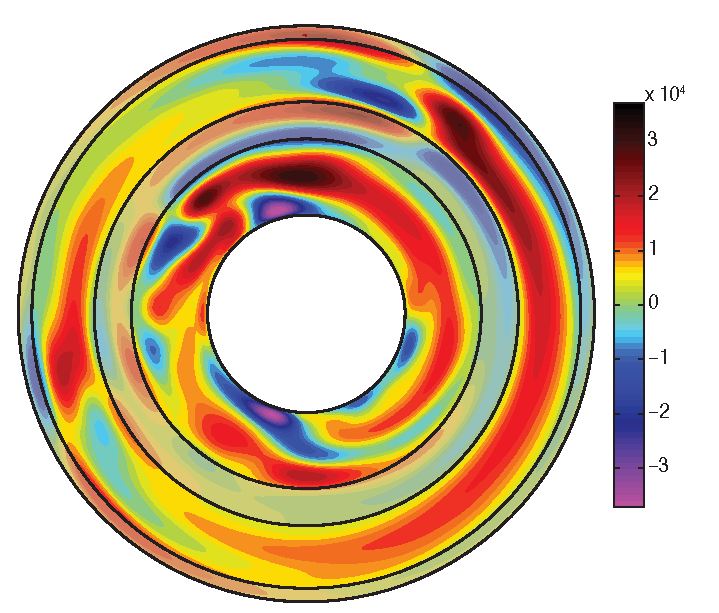
\includegraphics[width=.6\linewidth]{Chapter4/figures/wz19_043_2500_00.pdf}
	\caption{A snapshot of axial vorticity in the equatorial plane for a double snow state model (model 1). Here, the snow layers have been shaded grey. The units in this figure are non-dimensional.}
	\label{fig:vorticity}
\end{figure}
the axial vorticity in the equatorial plane is plotted. The regions of solid colour correspond to convection columns aligned with the rotation axis and the sign of the vorticity indicates the direction the column is rotating. The convection columns are coaxial with the rotation axis and do not cut across the stably stratified layer. Although there are patches of vorticity inside the stable layer, these are all due to viscous coupling to an opposite patch of vorticity in the convective region and do not contribute to dynamo generation processes.

The snow layer also has consequences for the axisymmetric flows. In figure \ref{fig:uax}
\begin{figure}
	\centering
	\noindent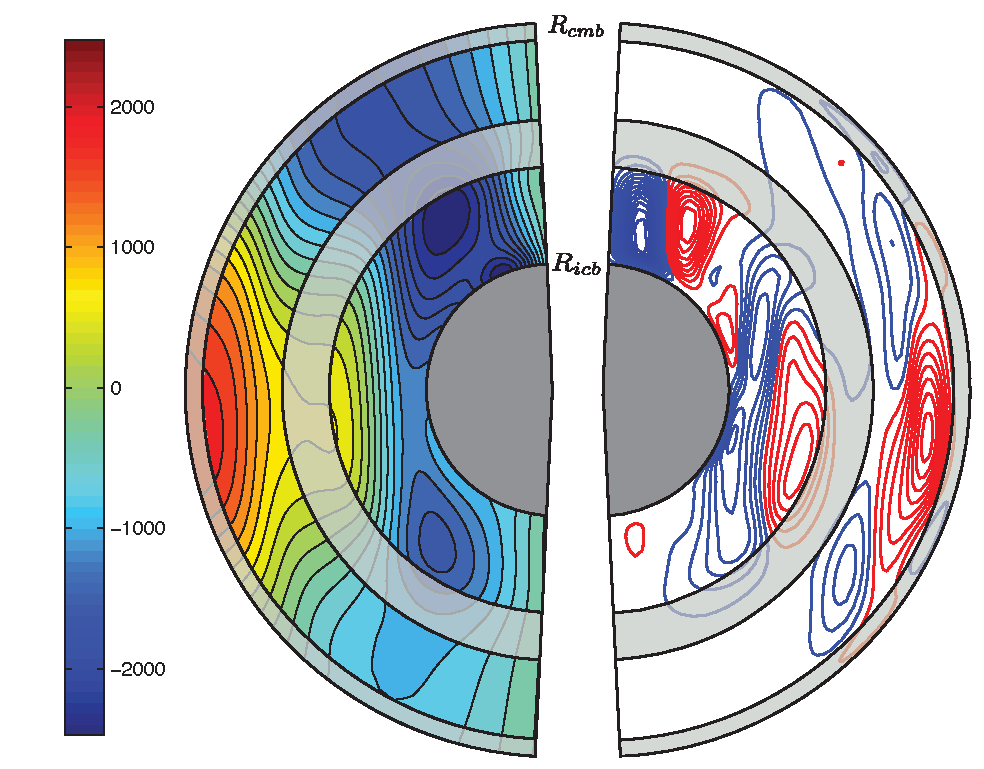
\includegraphics[width=.6\linewidth]{Chapter4/figures/uxtpavg19_043_2460-2530}
	\caption{Contours of the axisymmetric toroidal component of the velocity (left) and streamlines of the axisymmetric poloidal velocity (right) for a double snow state model, averaged over $0.35$ dipole magnetic diffusion times. In the right plot the colour denotes the direction of the flow, red is clockwise and blue is counterclockwise. Here, the snow layers have been shaded. The units in this figure are non-dimensional.}
	\label{fig:uax}
\end{figure}
 the axisymmetric toroidal (left) and poloidal (right) components of velocity are plotted. Examining the toroidal component of velocity, we see that the snow zones, especially the deep snow zone, bend the zonal flow contours significantly. The regions closest to the rotation axis are dominated by a retrograde flow, while the regions in the equatorial region near the CMB have an overall prograde flow. Examining the poloidal velocity field (figure \ref{fig:uax} (right)) we see that most of the poloidal flow occurs in the inner dynamo region. In the outer region, convection is concentrated in the equatorial region with little convection occurring inside the tangent cylinder formed by the deep snow layer. 

\subsection{Magnetic Field}
The nature of this dynamo is revealed if we examine the generation mechanisms for both toroidal and poloidal fields. Figure \ref{fig:maggen} (a) shows the axisymmetric toroidal field for a double snow state model.
%
\begin{figure}
	\centering
	\noindent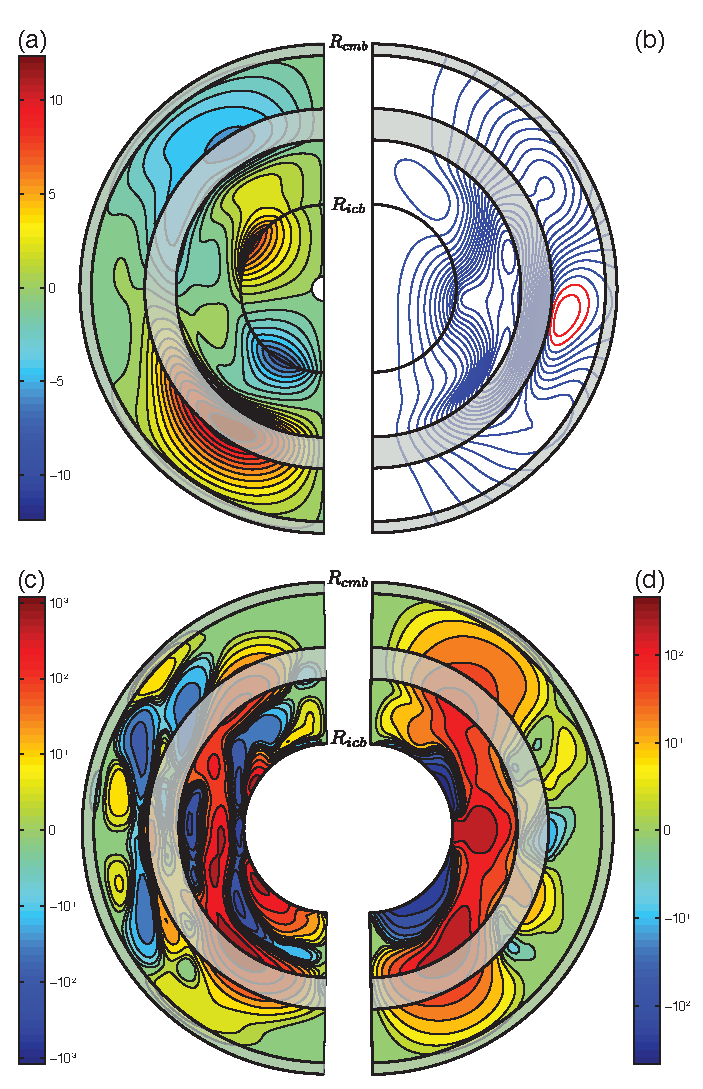
\includegraphics[width=.7\linewidth]{Chapter4/figures/aximaggen}
	\caption{(a) Contours of the axisymmetric component of the toroidal magnetic field for a double snow state model. (b) Streamlines of the axisymmetric poloidal field for a double snow state model. The colour of the streamline denotes the direction of the field, red is clockwise and blue is counterclockwise. (c) An axisymmetric slice of the generation of toroidal magnetic field energy due to stretching of poloidal magnetic field ($\overline{\mathbf{B}_{T}\cdot\left[\left(\mathbf{B}_{P}\cdot\nabla\right)\mathbf{u}\right]}$) for a double snow state model. (d) An axisymmetric slice of the generation of poloidal magnetic field energy due to stretching of toroidal magnetic field ($\overline{\mathbf{B}_{P}\cdot\left[\left(\mathbf{B}_{T}\cdot\nabla\right)\mathbf{u}\right]}$) for a double snow state model. All the plots in this figure are from model 1, and have been averaged over the same period as figure \ref{fig:uax}. The snow layers have been shaded grey. The units in this figure are non-dimensional.}
	\label{fig:maggen}
\end{figure}
%
When compared to an Earth-like model (i.e. no snow zones) (figure \ref{fig:toroidalpoloidalearth}, left), it appears as though there are two dynamos of opposite polarity operating within the same core of the double snow state model.
%
\begin{figure}
	\centering
	\noindent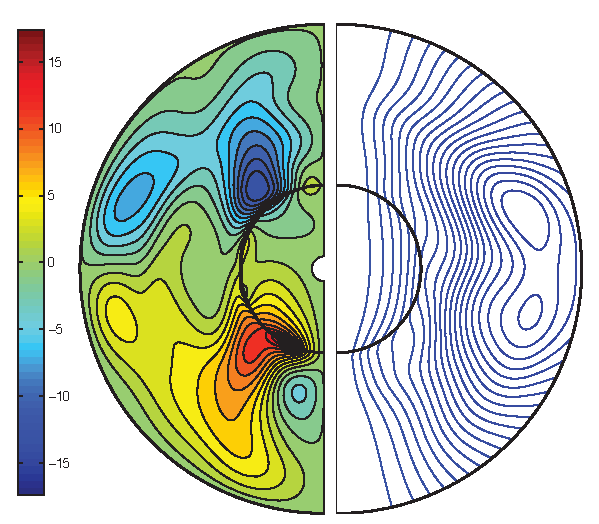
\includegraphics[width=.6\linewidth]{Chapter4/figures/BTorPolEarth}
	\caption{Contours of the axisymmetric component of the toroidal field (left) and streamlines of the axisymmetric poloidal field (right) for a snapshot of a strong field, Earth-like model (i.e. a model with no snow zones).  The units in this figure are non-dimensional.}
	\label{fig:toroidalpoloidalearth}
\end{figure}
%
Further evidence for this ``double dynamo'' interpretation is found by examining the radial magnetic field at the CMB (figure \ref{fig:brad}, top).
\begin{figure}
	\centering
	\noindent\includegraphics[width=\linewidth]{Chapter4/figures/Brad_dim.pdf}
	\caption{The radial magnetic field for model 1 at the CMB (top) and at  the surface (bottom) at the same instant in time as figure \ref{fig:vorticity}. The tangent cylinder formed by the deep snow layer has been shaded grey. }
	\label{fig:brad}
\end{figure}
In figure \ref{fig:brad} the intersection of the tangent cylinder formed by the deep snow zone with the CMB is shaded grey. We note that there seem to be no features in the radial magnetic field at the CMB from the tangent cylinder of the inner core \citep{stanleyfluxspot}, while the deep snow zone's tangent cylinder serves as the border between radial field of opposing sign. Also, the prominent flux spots in the equatorial region do not occur poleward of the tangent cylinder formed by the deep snow layer.

In figure \ref{fig:brad} (top), which plots the radial component of the magnetic field at the CMB for model 1, a strong octupolar signature is seen (figure \ref{fig:power}, Table \ref{tab:runs}).
\begin{figure}
	\centering
	\noindent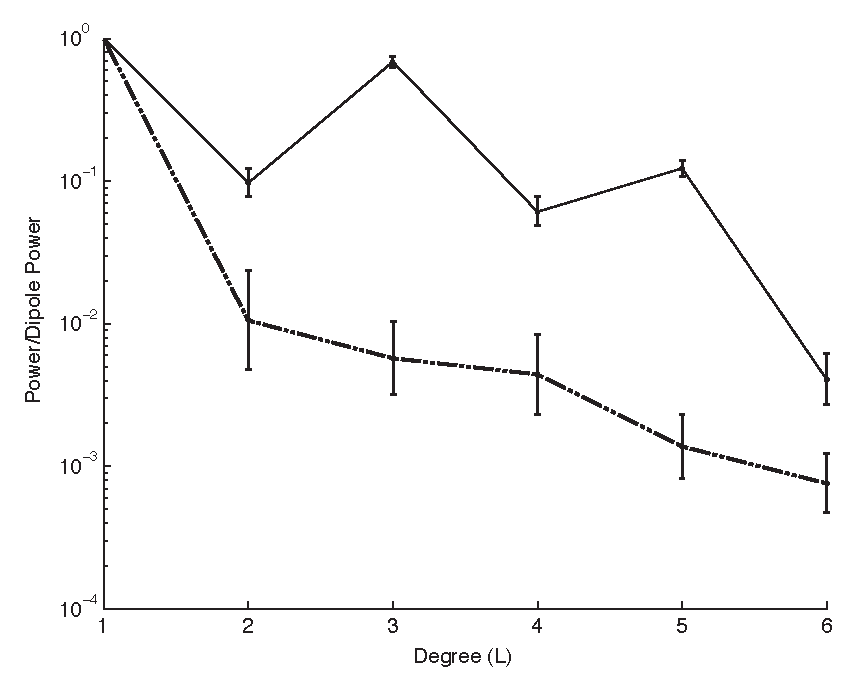
\includegraphics[width=30pc]{Chapter4/figures/powermodel.pdf}
	\caption{Temporally averaged surface power spectra for an Earth-like model (i.e. a model without snow zones) (dashed) and for a double snow state model (solid, model 1) averaged over the same time period as figure \ref{fig:uax} at the surface of a Mercury-like planet ($R_{\mathrm{cmb}}=0.75$). Both models have been averaged over $0.35$ dipole magnetic diffusion times. The error bars on the power spectrum for the model indicate one standard deviation of the power over the averaging window.}
	\label{fig:power}
\end{figure}
The magnetic field generated by the dynamo region nearest to the inner core is expressed in the polar regions, while the equatorial regions are dominated by the field generated in the outer dynamo region. If we observe the radial magnetic field for different radii inside the core,  the inverted polarity in the equatorial region does not appear until outside the deep snow zone, indicating a source in the outer dynamo region.

While the dipole moment of these dynamo models matches the dipole moment of Mercury quite well, the model $\mathrm{g}_2^0$ Gauss coefficient is not matched as well. In figure \ref{fig:gauss} we plot $\mathrm{g}_2^{0}$ against $\mathrm{g}_1^{0}$ at each timestep output by all of our double snow state models. The observations from the MESSENGER mission of $\mathrm{g}_1^{0}$, and $\mathrm{g}_2^{0}$ are shown as grey rectangles, with the size of the rectangles denoting the uncertainty associated with the measurements. In this figure there are two areas that match Mercury's magnetic field, this is due to the north-south symmetry present in the magnetic induction equation. The important value to match is the magnitudes and relative signs of these two Gauss coefficients. In figure \ref{fig:gauss} we see that model 1 briefly matches Mercury's magnetic field, however most of the time the $\mathrm{g}_2^0$ field component is too small or has the wrong sign to be compatible with the MESSENGER measurements. 
\begin{figure}
	\centering
	\noindent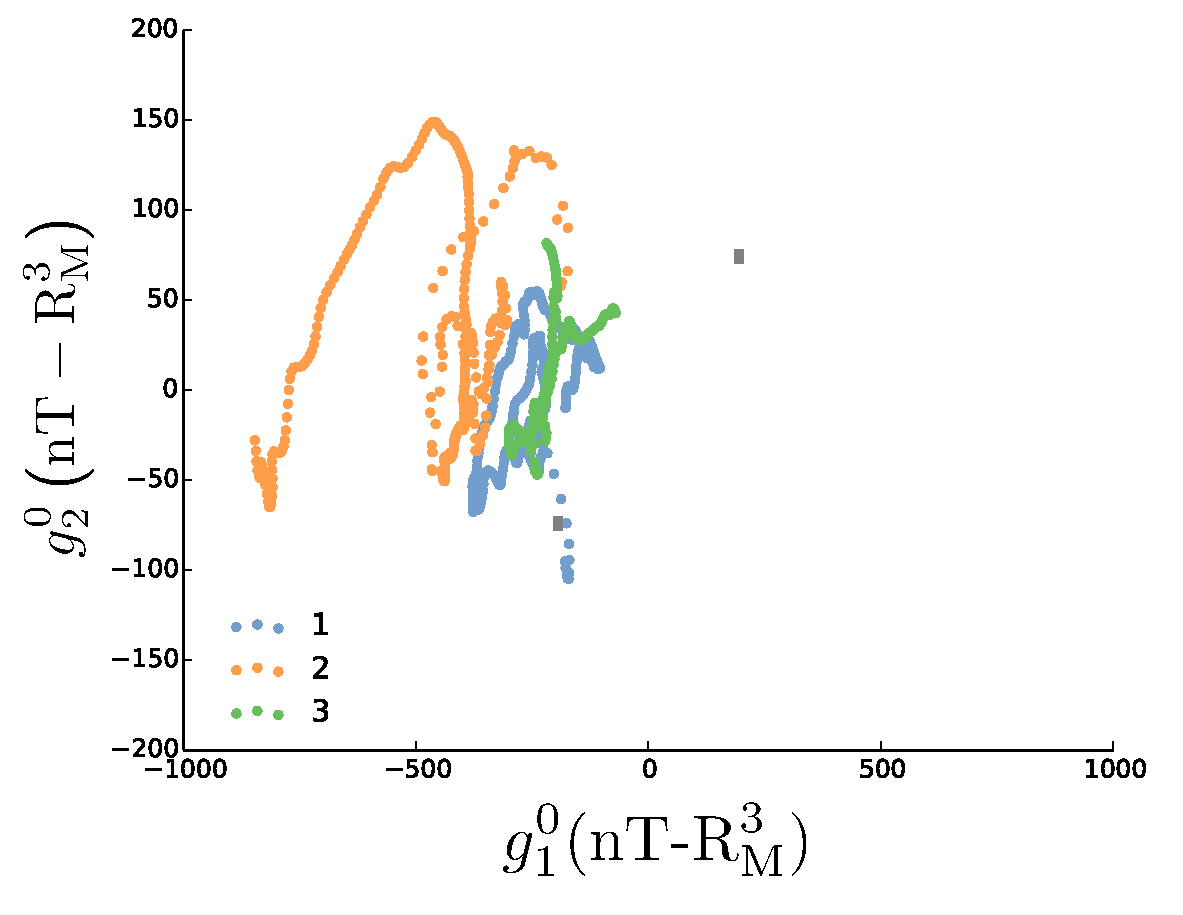
\includegraphics[width=30pc]{Chapter4/figures/g10g20.pdf}
	\caption{The axial dipole and quadrupole Gauss coefficients for the double snow state models in this study. The grey boxes denote areas of the plot which would match the MESSENGER observations of Mercury's magnetic field to within uncertainties. Here the numbers in the legend refer to the run numbers in Table \ref{tab:runs}.}
	\label{fig:gauss}
\end{figure}

\subsection{Dynamo Mechanism}
\subsubsection{Generation of the Toroidal Field}
The inverted polarity of the toroidal magnetic field in the outer region can be understood by examining the dominant $\omega$-effect component of the toroidal field generation in our models. From equation (\ref{eq:nondimmagnetic}), the growth of axisymmetric energy in the toroidal magnetic field can be written as
\begin{equation}
\mathbf{B}_{T}\cdot\frac{\partial \mathbf{B}_{T}}{\partial t}=\mathbf{B}_{T}\cdot\left[\left(\mathbf{B}\cdot\nabla\right)\mathbf{u}\right]-\mathbf{B}_{T}\cdot\left[\left(\mathbf{u}\cdot\nabla\right)\mathbf{B}\right].
\end{equation}
The first term on the right describes the growth of energy in the toroidal field due to stretching of magnetic field lines while the second describes the growth of toroidal field energy due to the advection of toroidal field. Focussing on the stretching term, the direction of the resultant toroidal field is dependent on the direction of the initial field and on the sign of the gradient of velocity which is shearing it. Figure \ref{fig:uax} (left) shows the axisymmetric toroidal component of the flow. Here, the stably stratified layer causes differential rotation in the $z$ direction. Examining the midlatitude regions where the flow is strongest, we see that the gradient in $\mathbf{u}$ changes sign just below the stable layer. An initially poloidal magnetic field which originates from the inner dynamo will be sheared by this differential rotation. The shear in the outer region will generate toroidal field which is opposite in sign to the toroidal field in the inner region. This process can be seen in figure \ref{fig:maggen} (c), which plots the axisymmetric growth of toroidal field energy caused by the stretching of poloidal magnetic field lines ($\overline{\mathbf{B}_{T}\cdot\left(\mathbf{B}_{P}\cdot\nabla\right)\mathbf{u}}$). We see that significant amounts of poloidal field are converted into toroidal field in the mid-latitudes of the outer region and deep snow layer, effectively seeding the outer region with toroidal field. Although there are other ways that toroidal field can be generated in the outer region (for example by stretching toroidal field) this is the dominant method in our models. Figure \ref{fig:schematictoroidal} shows a schematic diagram of this process.
\begin{figure}
	\centering
	\noindent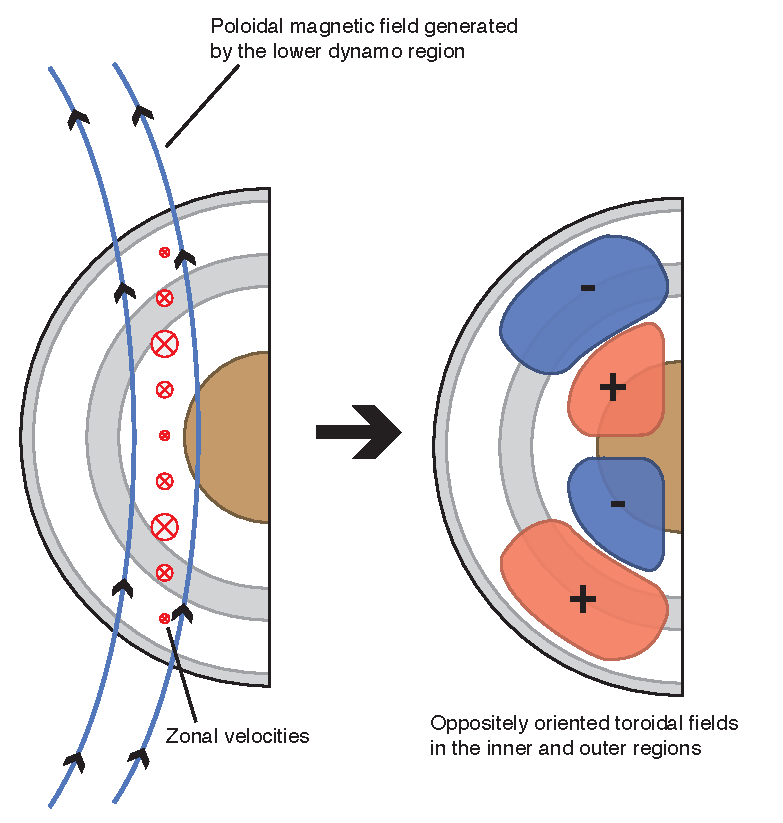
\includegraphics[width=30pc]{Chapter4/figures/Schematic-Toroidal.pdf}
	\caption{A schematic diagram of the generation of the toroidal field in a double snow state model. On the left, red arrowheads (going into the page) represent zonal velocities whose strength is proportional to the arrow head size. Moving in the direction of the poloidal field line, an increase in zonal velocity (i.e. a positive gradient) results in  positively signed toroidal field generation. Conversely, a decrease in zonal velocity (i.e. a negative gradient) results in negatively signed toroidal field generation. These act on poloidal magnetic fields (blue) to create the characteristic toroidal field we observed in our models. The snow layers have been shaded grey.}
	\label{fig:schematictoroidal}
\end{figure}

\subsubsection{Generation of the Poloidal Field}
Poloidal fields in both the inner and outer regions are generated by convective motions acting on toroidal fields. In the inner region, convection is stronger and a strong dipolar field is generated. However, the dipole field observed outside the core is weak due to a combination of three processes, which all stem from the presence of a deep snow layer. A schematic diagram illustrating these three processes is shown in figure \ref{fig:schematicpoloidal}.
\begin{figure}
	\centering
	\noindent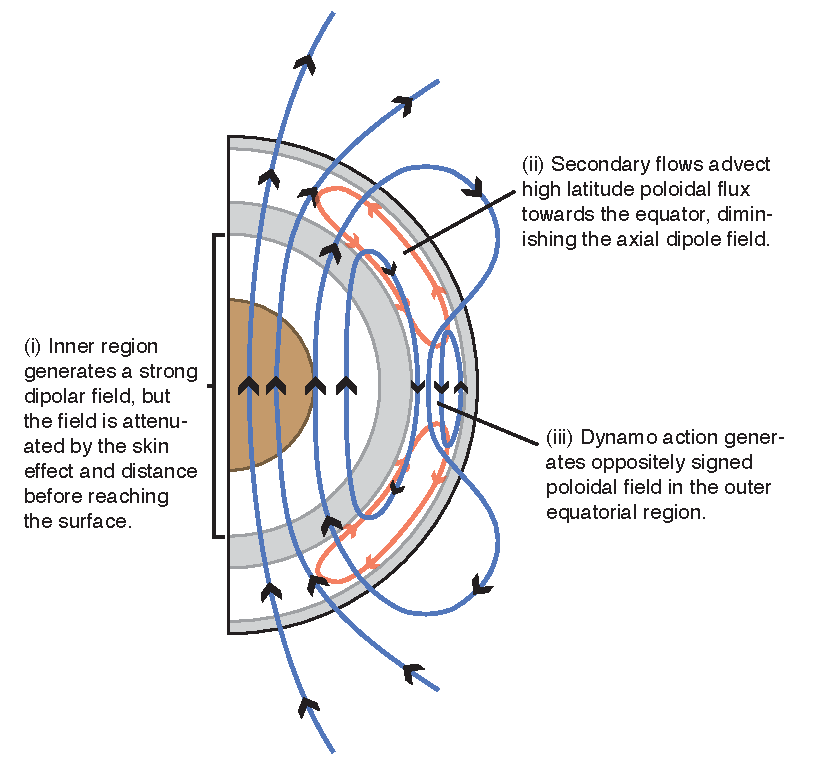
\includegraphics[width=30pc]{Chapter4/figures/Schematic-Poloidal.pdf}
	\caption{A schematic diagram of the generation of the poloidal magnetic field in a double snow state model. In this figure blue lines represent poloidal magnetic field lines, and red lines represent meridional flows. The three mechanisms discussed in the text for weakening the observed field are marked (i), (ii), and (iii). The snow layers have been shaded grey.}
	\label{fig:schematicpoloidal}
\end{figure}

First, the inner dynamo region does most of the field generation, but since it is removed from the CMB (due to the presence of the outer layer), its strength is reduced. This is similar to the mechanism behind the weak magnetic field observed in \citet{christensen06} however, this is not the sole reason for the overall weakness of the field in our models. In  \citet{christensen06} the parameters were chosen such that magnetic field at the top of the dynamo generation region was both strong and non-dipolar. Although placing the dynamo generation away from the surface does weaken the dipole moment observed at the surface, the primary reason their model possesses a weak dipole moment is because most of the power lies in higher multipoles which vary quickly in time and are preferentially attenuated due to the screening effect. To determine whether our fields are weak solely due to the screening effect (section \ref{sec:screeningderiv}), we ran a deep snow state model, in which the region above the lower boundary of the deep snow zone was strongly stably stratified. This ensured that no dynamo action would occur in the outer region, and that any weakening of the field observed would be solely due to the screening effect or the removal of the dynamo region from the surface. We found that when we did this, the magnetic field was stronger than in our models containing a convective upper region by approximately an order of magnitude. From this analysis we conclude that flows in the outer region play an important role in the attenuation of the overall field in our models.

Secondly, additional weakening of the dipole moment in our models occurs through the theft of flux by meridional flows in the outer dynamo region. The density of poloidal magnetic field lines is reduced in the mid-latitudes of the outer region in figure \ref{fig:maggen} (b), as the field lines are advected towards the equator by meridional flows in this region (see figure \ref{fig:schematicpoloidal} for a schematic representation of this).

Finally, dynamo action in the outer region weakens the observed surface field. The conversion of the toroidal field in the mid-latitudes of the outer region into poloidal field can be seen when we plot the axisymmetric growth of poloidal field energy caused by the stretching of toroidal magnetic fields ($\overline{\mathbf{B}_{P}\cdot\left(\mathbf{B}_{T}\cdot\nabla\right)\mathbf{u}}$) which is plotted in figure \ref{fig:maggen} (d). When this is compared with the axisymmetric streamlines of poloidal magnetic field in figure \ref{fig:maggen} (b) we see that the source of the equatorial poloidal field we observe is the mid-latitude toroidal flux sheared out by the snow layer. Since the outer dynamo region is seeded with toroidal field which is opposite in polarity to that of the inner dynamo region, convection will generate a poloidal field in the outer region of opposite sign to the field generated by the inner region. Evidence that the outer dynamo region would operate in this way comes from studies of dynamos in thin shells (similar to the geometry of the outer shell) which show that at similar Rayleigh numbers to the ones used here, dipolar fields result \citep{stanleyandmohammadi}. In the outer region we observe a very similar field morphology as \citet{stanleyandmohammadi}, implying that if both regions generated poloidal field independently, the resulting fields would be of opposite polarity. Since they occur within the same core, they superpose and contribute to the weak observed surface field. 

The polarity of the outer dynamo is entirely determined by the inner dynamo. Since the outer region is being primed with a toroidal field by the inner region, and since convection is relatively weak in the outer region, it is unlikely that this dynamo could ever determine it's polarity independent of the inner region. The situation of a dynamo being immersed in an externally applied field was examined by \citet{sarson97}. In that case a dynamo was immersed in a constant background field, giving the dynamo an external source of poloidal field, which it could then convert to toroidal field. In our case the opposite occurs, the inner dynamo region supplies the outer dynamo region with a toroidal field which this region then converts to poloidal field. 

When a double snow state model reverses, it is the inner dynamo that leads the reversal. During the reversal, the dipole moment decays to only a few nT-$R_{M}^3$. After the reversal finishes, the same differential rotation in $z$ occurs, so the outer dynamo region once again becomes active with the opposite sign as the inner dynamo region. 

In our models we chose parameters such that the magnetic Reynolds numbers of our snow zone models are comparable to the Earth-like dynamo model in figure \ref{fig:toroidalpoloidalearth}. We define our magnetic Reynolds number as
\begin{equation}
\mathrm{Re}_{M}=\frac{1}{V}\int_{V}\frac{\left|\nabla\times\left(\mathbf{u}\times\mathbf{B}\right)\right|}{\left|\nabla^{2}\mathbf{B}\right|}.
\end{equation}
We have done this to ensure that any change in field strength we observe is not the result of a different efficiency of magnetic field generation. The difference in the field intensity at the surface can therefore be attributed to the change in field morphology resulting from the snow zones. Other studies  \citep{christensen06scaling} have shown that Earth-like dynamo models have a critical magnetic Reynolds number of order 50. The Earth-like dynamo model in figure \ref{fig:toroidalpoloidalearth} and our double snow state models have magnetic Reynolds numbers in the range of $48$-$62$.

\section{Discussion}
We have shown that introducing exotic (yet predicted) sources of compositional driving can produce a dipole moment as weak as the measured moment of Mercury. Although both the deep and double snow states produced dipole moments weaker than one would expect from scaling arguments, the double snow states most closely match the observations of Mercury. The deep snow state is also less likely than the double snow state due to the high ($>10\%$wt) sulphur content it requires \citep{rivoldini09}. The results of this work are published in \citet{vilim2010}.

Owing to the reduction in length scale caused by the addition of the stably stratified layer, our models in a double or deep snow state geometry must operate at Rayleigh numbers which are more than $40$ times supercritical in order to sustain a magnetic field against ohmic decay. For example, although they use a slightly different geometry and different boundary conditions, \citet{christensen06} show that $\mathrm{Ra}>50\mathrm{Ra}_{c}$ for dynamo onset in the parameter regime of our snow zone models (in order to make this comparison, one must convert our definition of the Ekman number to one in terms of shell thickness rather than core radius, using the thickness of the lower dynamo region as the shell thickness). Since we must operate at highly supercritical Rayleigh numbers, we must turn to hyperdiffusivities for computational reasons. We have run high resolution calculations  ($L_{max}=90$, $m_{max}=85$, $n_{r}=65$) at lower ($7.9 Ra_{c}$) supercritical Rayleigh numbers with minimal ($l_{o}=40$, in equations (\ref{eq:hyperdiffseta})-(\ref{eq:hyperdiffsnu})) or absent hyperdiffusivities, however these supercriticalities are too low to sustain magnetic fields. The absence of dynamo action at these low Rayleigh numbers when hyperdiffusivites are not used implies that small scale fluid motions, which are preferentially damped in our models that use hyperdiffusivities, are not responsible for the large scale field generation.

The mechanisms behind the formation of the dynamo state we observe are expected to be robust with regard to the implementation of hyperdiffusivities. Fluid motions in the lower dynamo region should produce a dipolar seed field irrespective of whether hyperdiffusivities are present. The principle reason for the pattern of toroidal fields we observe in our study is differential rotation in the radial direction at mid-latitudes. Finally, the transport of flux towards the equator is caused by large scale secondary flows which occur in dynamos without hyperdiffusivies as well. 

This system is likely to evolve in time substantially. Over long timescales the upper dynamo region should become preferentially enriched in sulphur and the lower region should become preferentially enriched in iron and eventually stratified down to the ICB as the zone of potential snow formation grows with cooling. Furthermore, the region nearest the CMB could form a stratified layer of light element similar to the kind proposed for the Earth \citep{Braginsky2006}. This stratified ocean would co-exist with the stratified region which we have already placed near the CMB. All these effects vary on timescales much longer than those associated with the dynamo, so they have been neglected here. Future work will focus on understanding the long term thermal and compositional evolution of a double snow state system. However, should future observations of Mercury's magnetic field confirm field characteristics consistent with the double snow zone model, this would place important constraints on the present-day structure of the planet's core.

In this study we have only examined situations that result in the outer dynamo region generating little field on its own. Understanding the consequences of increasing the Rayleigh number, which should lead to an increase the vigor of convection in the outer dynamo region will be an area of interesting future research.

The magnetic field produced by a geometry containing a deep snow layer is quite distinct. For the $r_{io}$ value used in this study ($0.34$), the octupole component is always much larger than the quadrupole component and is comparable to the dipole component.


















%!TEX root = ../thesis.tex

\chapter{Iron Flotation Layers in Mercury}
\label{chap:floatationlayers}
A model to explain the strength of Mercury's magnetic field was proposed by \citet{smith2012} using gravitational data from the MESSENGER probe. They synthesised observations of Mercury's gravitational moments, as well as moment of inertia measurements derived from Earth based observations of Mercury's rotational state to construct an interior model of Mercury. Their inversions revealed the possibility of a deep, dense layer in Mercury's mantle. They proposed that this layer is composed of FeS, which solidified and floated on Mercury's bulk core due to the unique way which Mercury's core may be freezing. They proposed this layer would attenuate the dynamo generated magnetic field via the skin effect before it reached the surface, producing Mercury's weak observed magnetic field. In this section we will implement this deep, dense, electrically conducting mantle in a numerical dynamo model to learn whether it can help explain Mercury's weak observed magnetic field.

\section{Gravity }
Gravitational measurements provide an important tool for learning about the structure of planets. Because the gravity field is a superpostition of the field from all the material in the planet, it is sensitive to the deep interior of the planet. While gravitational inversions are not unique, they can be combined with other measurements to help constrain interior structure models.

\subsection{Introduction to Gravity}
Because the gravitational force is irrotational ($\nabla \times\mbf{g}=0$, where $\mbf{g}$ is the acceleration due to gravity) we can write it as the gradient of a scalar potential
\begin{equation}
\mbf{g}=-\nabla\Phi.
\end{equation}
In section \ref{sec:representations} we showed that this means $\Phi$ is a solution to Laplace's equation, which allows us to expand the angular part in a spherical harmonic expansion. The gravitational spherical harmonic expansion is usually written as 

\begin{equation}
\Phi\left(\mbf{r}\right)=-\frac{GM}{r}\left\{1-\sum_{l=1}^{\infty}\sum_{m=0}^{l}\left(\frac{a}{r}\right)^{l}P_{l}^{m}\left(\cos\theta\right)\left[C_{l}^{m}\cos\left(m\theta\right)+S_{l}^{m}\sin\left(m\theta\right)\right]\right\}
\label{eq:gravityexpansion}
\end{equation}
where $G$ is the gravitational constant, $M$ is the mass of the planet, $a$ is the planets equatorial radius, and $P_l^m$ is a Schmidt normalised associated Legendre polynomial. Here $C_l^m$ and $S_l^m$ are known as the gravitational moments, which can be computed by
\begin{equation}
\left\{
\begin{array}{c}
C_l^m\\
S_l^m
\end{array}
\right\}=-\frac{1}{M}\int_{V}\rho\left(r,\theta,\phi\right) \left(\frac{r}{a}\right)^l P_{l}^{m}\left(\cos\theta\right)\left\{
\begin{array}{c}
\cos m\theta\\
\sin m \theta
\end{array}
\right\}
dV.
\label{eq:gravitycoefficients}
\end{equation}
Importantly these are sensitive to the density distribution of the planet. We see that in equation \ref{eq:gravitycoefficients} the density $\rho$ is weighted by $\left(r/a\right)^l$. This means that the shallower layers of the planet (where $r/a\approx 1$) have a greater effect on the higher harmonics than the deeper layers.

There are two other important notes we will make concerning equation \ref{eq:gravityexpansion}. First, if we pick the origin of our coordinate system to coincide with the centre of mass of our body, the components with $l=1$ vanish (we will do this from now on). Second, the gravitational harmonics of degree 2 can be related to the moments of inertia of the planet. Specifically, if $A$, $B$, and $C$ are the moments of inertia around the three principal axes of the planet we can write
%Specifically, if $I_{jk}$ denotes the components of the moment of inertia tensor in cartesian coordinates, the diagonal elements $I_{11}, I_{22}, I_{33}$ represent the moments of inertia around the three principal axes $A$, $B$, $C$ respectively. We can also relate the gravitational moments to the moments of inertia as
\begin{align}
C_2^0&=\frac{A+B-2C}{2a^2 M} \label{eq:C20}\\
%C_2^1&=\frac{I_{13}}{a^2 M}=\frac{I_{31}}{a^2 M} \\
%S_2^1&=\frac{I_{23}}{a^2 M}=\frac{I_{32}}{a^2 M} \\
C_2^2&=\frac{1}{4a^2 M} \left(B-A\right). \label{eq:C22}
%S_2^2&=\frac{1}{2 a^2 M} I_{12} = \frac{1}{2 a^2 M} I_{21}
\end{align}
For further details regarding this derivation see \citet{kaula1968}.

\section{Physical Librations of Mercury}
Because Mercury orbits so closely to the sun, it experiences gravitational torques associated with its permanent deformation. This causes a longitudinal libration in Mercury's spin which can be related to the moments of inertia
\begin{equation}
\phi_{0}=\frac{3}{2}\left(\frac{B-A}{C}\right)\left(1-11e^2+\frac{959}{48}e^4+\ldots\right)
\label{eq:librationamp}
\end{equation}
where $\phi_{0}$ is the amplitude of the libration, and $A$, $B$ and $C$ are the moments of inertia around the principle axes \citep{peale1972}. As we discussed in chapter \ref{chap:doublesnowstates}, \citet{margot2007} showed that the amplitude of the libration is too large to be explained if Mercury's core participates in the libration, implying an outer shell that librates independently of a core which is at least partially liquid. This means that $C=C_m$ in equation \ref{eq:librationamp}, where $C_m$ is the polar moment of inertia of the solid mantle and crust layer.

\citet{margot2007} also showed that Mercury is in a Cassini state 1, where spin axis and orbit normal are co-linear and are normal to the orbital plane. This means that the relation
\begin{equation}
K_1\left(\theta\right)\left(\frac{C-A}{C}\right)+K_2\left(\theta\right)\left(\frac{B-A}{C}\right)=K_{3}\left(\theta\right)
\label{eq:kconstraint}
\end{equation}
holds \citep{peale1969}. In equation \ref{eq:kconstraint}, $A$, $B$, and $C$ are the moments of inertia about the principal axes of the entire planet (not only the outer shell). Also, $K_1\left(\theta\right)$, $K_2\left(\theta\right)$ and $K_3\left(\theta\right)$ are known functions that only depend on the obliquity ($\theta\approx0$). Full expressions for these functions can be found in \citet{peale1969}.

\section{Determining the Interior Structure of Mercury}
We can rearrange equation \ref{eq:kconstraint} and use the expressions for $C_2^0$ and $C_2^2$ to give
\begin{equation}
\label{eq:mr2c}
\frac{M R^2}{C}=\frac{K_3\left(\theta\right)}{K_1\left(\theta\right)\left(2C_2^2-C_2^0\right)+K_2\left(\theta\right)\left(4C_2^2\right)},
\end{equation}
then use equation \ref{eq:librationamp} to get,
\begin{align}
\label{eq:bacm}
\frac{B-A}{C_m}\approx\frac{2}{3}\phi_{0}
\end{align}
and finally rearrange equation \ref{eq:C22} to give
\begin{equation}
\label{eq:bamr2}
\frac{B-A}{MR^2}=4C_2^2.
\end{equation}
Since the right hand side equations \ref{eq:mr2c}, \ref{eq:bacm} and \ref{eq:bamr2} are all known quantities, some simple algebra yields
\begin{equation}
\frac{C_m}{C}=\left(\frac{C_m}{B-A}\right)\left(\frac{B-A}{MR^2}\right)\left(\frac{MR^{2}}{C}\right),
\end{equation}
which represents the ratio of polar moments of inertia of the mantle shell and the entire planet. If this ratio is less than 1 it means that the surface and the core are de-coupled, implying a liquid layer.

\citet{smith2012} constructed a suite of models which attempted to match the values of $C_m/C$ and $C/MR^2$ observed for Mercury. Their best fit model implied a liquid core which extended to a radius of $2030 \pm37 \textrm{km}$, and a solid mantle/crust which extended to the surface ($2440\textrm{km}$). They also found that the mantle shell has a density of $3650\pm225 \textrm{kg}/\textrm{m}^3$, which is larger than expected given the low iron abundance measured at Mercury's surface \citep{nittler2011}.

A solution that they proposed was that there could be a dense layer deep within Mercury's mantle that accounts for this disparity in density. They suggested that recent research suggesting the immiscibility of Fe-Si-S at Mercuy's core conditions would result in a sulphur rich liquid layer at the top of Mercury's core. This layer would then solidify FeS which could float on top of the bulk liquid, accumulating at the core mantle boundary. They propose that this layer could range from $10\textrm{km}$ to as much as $200\textrm{km}$ in thickness while still being compatible with the moment of inertia values that they report.

They then argue that because this solid, FeS layer conducts electricity it may provide a mechanism to reduce the field strength of Mercury's magnetic field by the same electromagnetic screening mechanism as \citet{christensen06}. 

While more recent studies such as \citet{hauck2013} have argued that the mantle density proposed by \citet{smith2012} is higher than the most probable mantle density, the density of \citet{smith2012} is not excluded by these updated measurements. It is therefore worthwhile to test the consequences of this proposed deep, solid FeS layer on magnetic field generation in Mercury.

\section{The Consequences of a Deep FeS Layer on Magnetic Field Generation in Mercury}
Before we run any numerical models with a deep, solid FeS layer there are a number of points regarding this model which merit discussion. First, the mechanism that \citet{smith2012} proposes to reduce the observed magnetic field strength of the dynamo is the electromagnetic screening mechanism proposed by \citet{christensen06}. A crucial difference between these studies is that the layer in \citet{christensen06} occupied $530\textrm{km}$ of Mercury's core, while the proposed solid FeS layer must be less than $200\textrm{km}$ to be compatible with observations. As we discussed in chapter \ref{chap:superearth}, a solid electrically conducting layer above the core reduces the magnetic field strength by a factor of $e^{-d\sqrt{\omega/(2 \eta)}}$ where $\omega$ is the frequency of the magnetic field variations at the top of the core, $d$ is the thickness of the conducting mantle and $\eta$ is the magnetic diffusivity. From this we see that a thinner layer will screen less magnetic field than a thicker layer and if that were the only effect in play it would seem that this proposed layer is insufficient to produce Mercury's weak magnetic field. The observable magnetic field in \citet{christensen06} was weakened further because the dynamo region was confined to a deep region of the core. Since multipoles of the magnetic field decay in space as $\left(r/a\right)^{l+2}$, the higher multipoles are attenuated more than the dipole field is at the surface. 

\citet{christensen06} argued from local Rossby number considerations that Mercury should be in a parameter regime that generates a multipolar magnetic field in which the small scale components vary quickly in time. This was crucial to their model, as a dipolar magnetic field would not vary quickly enough to be effectively attenuated by the screening mechanism. Due to computational restrictions \citet{christensen06} ran their numerical models at local Rossby numbers of $\mathcal{O}\left(10^{-1}\right)$ instead of the true local Rossby number of Mercury ($\mathcal{O}\left(10^{1}\right)$, \citep{OlsonandChristensen2006}). Qualitatively, an increase in the local Rossby number has the tendency to make dynamo generated magnetic fields smaller scale and more highly time variable. This means that a thin conducting layer can have the same screening effect as a thicker conducting layer if the timescale of the magnetic field variation is decreased by running a dynamo model at a higher, more accurate local Rossby number. 

We can quantify the relationship between timescale and local Rossby number by combining two scaling laws which exist in the literature. First, a scaling law by \citet{christensen2004} related the spherical harmonic degree ($L$) and the magnetic Reynolds number ($Rm$) to the timescale of variation of the dynamo
\begin{equation}
\tau\propto Rm^{-1} L^{-1}
\end{equation}
where $\tau$ is defined as
\begin{equation}
\label{eq:timescale}
\tau=\sqrt{\frac{\langle \sum_{L, m} \left(g_{Lm}^2+h_{Lm}^2\right)\rangle}{\langle \sum_{L, m} \left(\dot{g}_{Lm}^2+\dot{h}_{Lm}^2\right)\rangle}}
\end{equation}
where overdots refer to time derivatives. Second, the appropriate manipulations of scaling laws by \citet{aubert2009} can relate the local Rossby number to the magnetic Reynolds number as
\begin{equation}
Rm\propto Ro_{l}^{0.875}
\end{equation}
meaning
\begin{equation}
\tau\propto Ro_{l}^{-0.875} L^{-1}.
\label{eq:timescalescalinglaw}
\end{equation}
Equation \ref{eq:timescalescalinglaw} implies that simulations at a higher, more realistic local Rossby number should have shorter timescales than simulations at lower local Rossby numbers. This means that the thinness of the FeS layer may not preclude the model of \citet{smith2012} from explaining Mercury's weak magnetic field.

The second mechanism present in these simulations is the Lorentz force coupling that we discussed in chapter \ref{chap:superearth}. This effect was not discussed in \citet{smith2012} or \citet{hauck2013} and is potentially quite important.  The assumptions governing the model of \citet{smith2012} rely on the dynamo generating a multipolar magnetic field which would then be efficiently screened by the solid electrically conducting layer. In chapter \ref{chap:superearth} we saw that a dynamo surrounded by an electrically conducting layer is greatly affected by the Lorentz stretching that occurs at the core-mantle boundary. This magnetic field stretching causes an increase in the axisymmetric toroidal magnetic field near the core-mantle boundary. This can only be converted to a non-axisymmetric poloidal field which we showed using the Bullard-Gellman formalism (Appendix \ref{chap:appendix1}). This non-axisymmetric field is then advected by the background zonal flows and appears as a time varying magnetic field to the solid electrically conducting layer in the stationary mantle frame, and is screened accordingly. The magnetic field at the surface is then weaker than it would have been if the mantle was electrically insulating.

One key assumption of the model we discussed in chapter \ref{chap:superearth} was that the dynamo was operating in a parameter regime which would produce a dipolar magnetic field in the absence of an electrically conducting mantle. The effect of a change in local Rossby number regime is difficult to predict and will need to be explored using numerical dynamo simulations, which we will discuss in the next section.

\section{Model}
\label{sec:fesmodel}
To simulate the core of Mercury in an FeS flotation scenario we ran a suite of simulations covering a range of local Rossy numbers. For each set of control parameters we run one simulation that includes an FeS flotation layer and a control model that does not. In all cases we choose an inner core size of $r_i=0.5r_o$. As we discussed in chapter \ref{chap:doublesnowstates}, the size of Mercury's inner core is almost completely unconstrained so an inner core size of $r_i=0.5r_o$ is a reasonable choice. For the models that include an FeS flotation layer we choose the thickness of this layer to be $89$km (extending from $r_o$ to $1.04r_o$), which is compatible with the results of \citet{hauck2013}. We also set the electrical conductivity of this layer to be constant in space and equal to the electrical conductivity of the core. The geometry of the model we consider here is visualised in figure \ref{fig:FeSSchematic}.
\begin{figure}
	\centering
        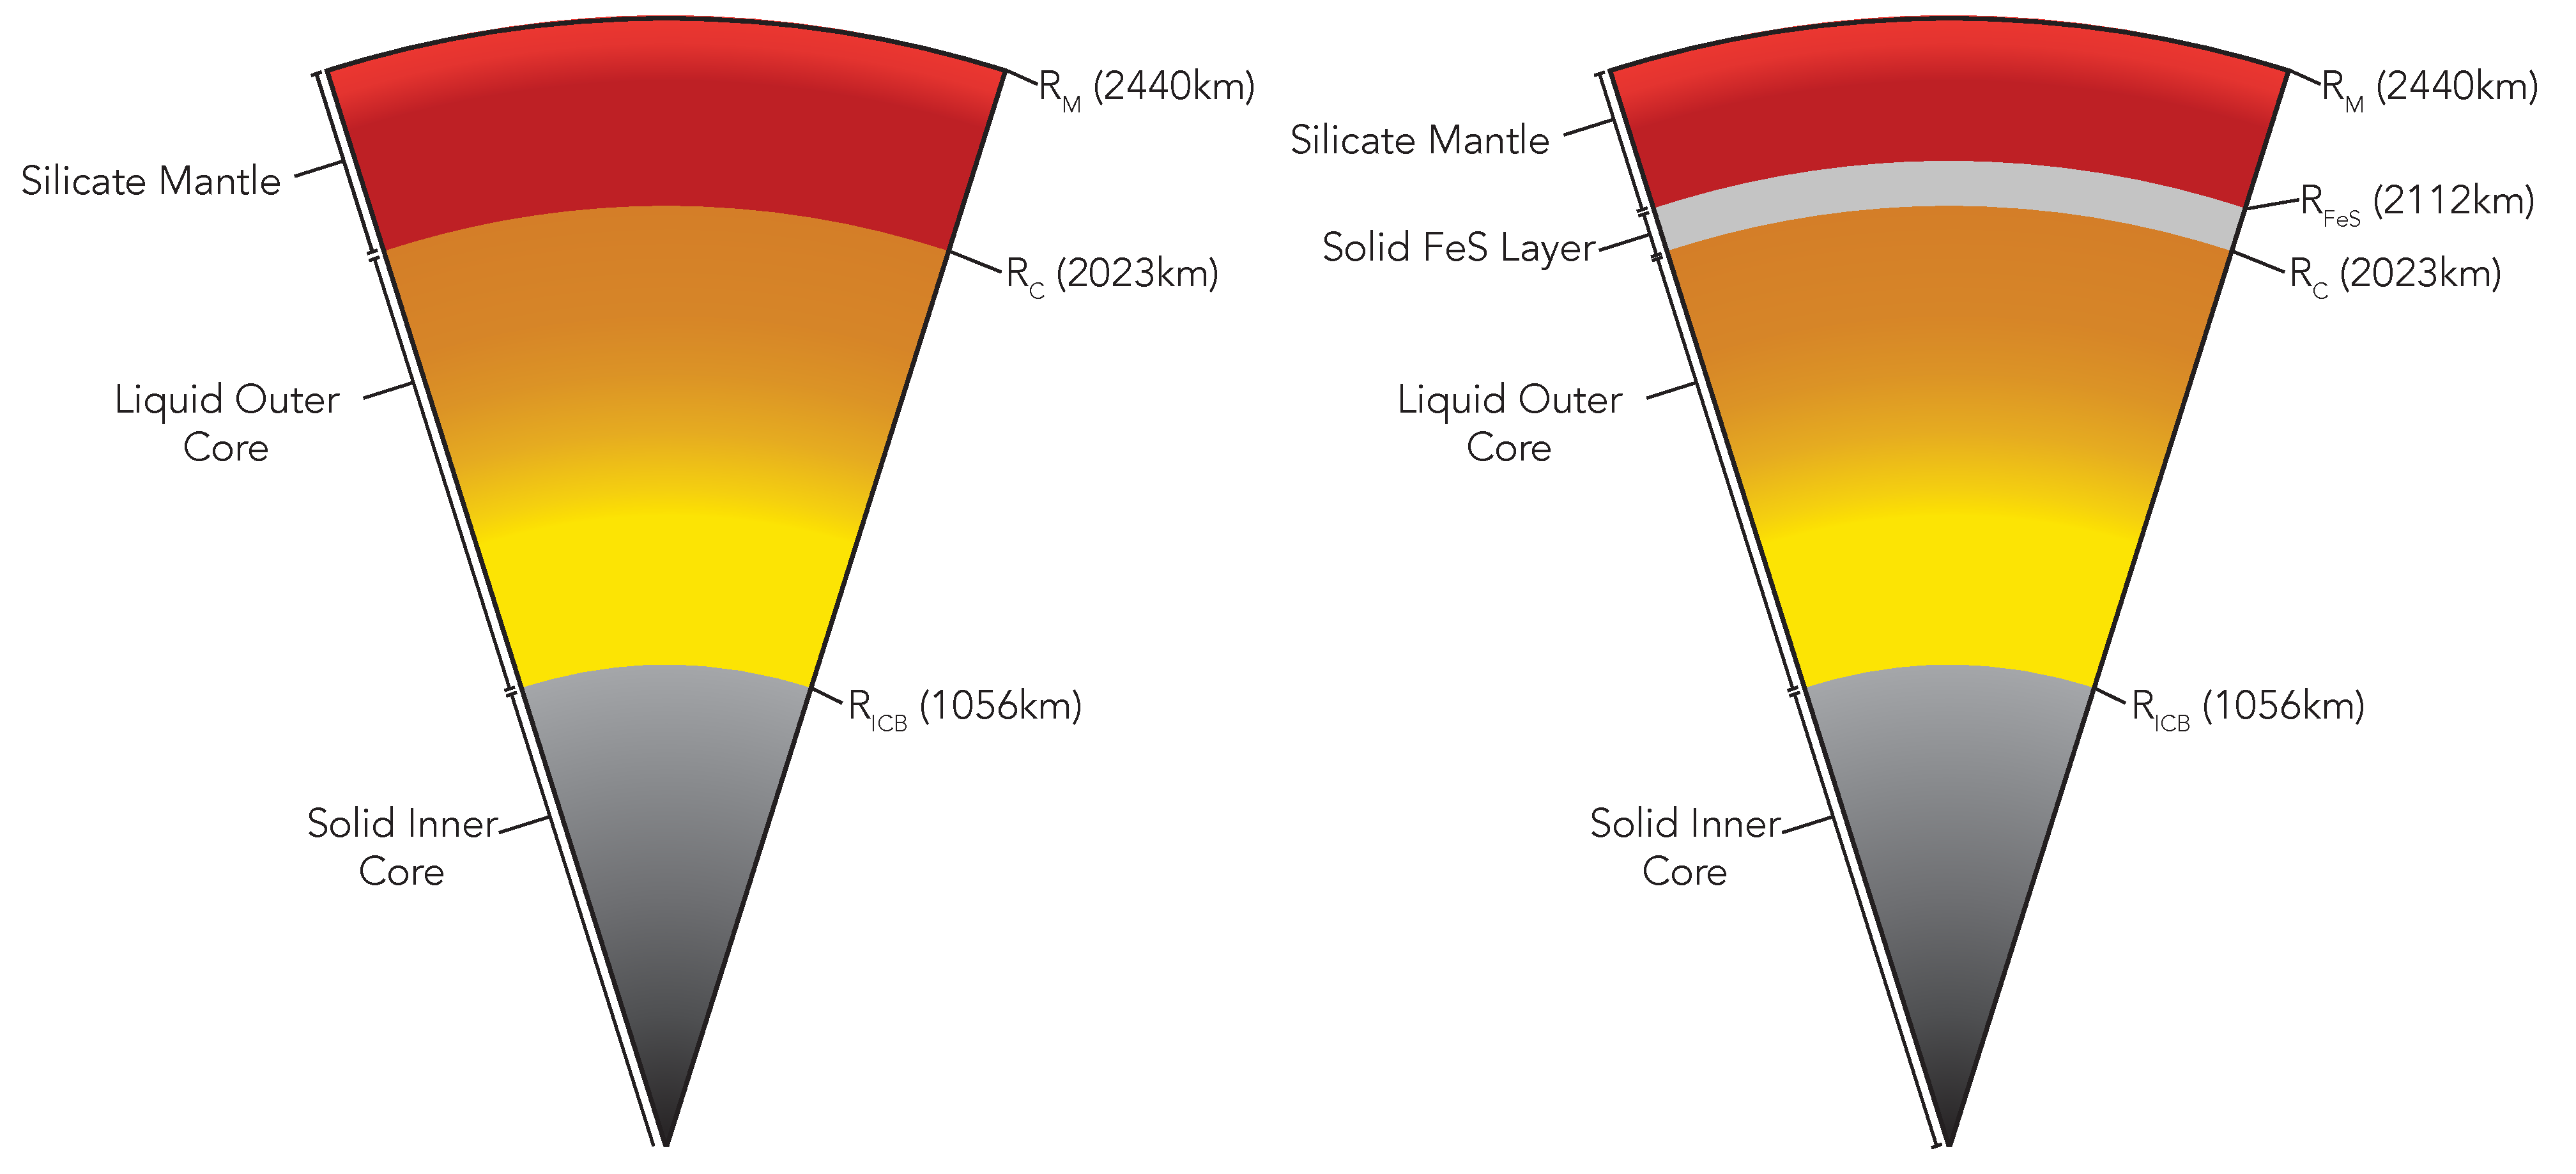
\includegraphics[width=\textwidth]{Chapter5/Figures/Structure.pdf}
        \caption{A schematic diagram of the models of Mercury's core presented in this chapter, without a FeS flotation layer (left) and with an FeS flotation layer (right).}
        \label{fig:FeSSchematic}
\end{figure}

All the simulations in this chapter were performed using the mMoSST numerical dynamo model. In these models the mantle was held fixed relative to the rotating planet frame, and the inner core was allowed to freely rotate due to magnetic and viscous torques. All fields (velocity, magnetic and co-density fields) were expanded to $L=100$ and $m=95$, and the inner core, fluid outer core and solid mantle layer have $75$, $80$ and $25$ radial gridpoints respectively. No hyperdiffusivities were used in any of the simulations in this chapter and the the non-axisymmetric inertial force is considered for all modes (see section \ref{chap:dynamotheory}).

In all cases, no-slip velocity boundary conditions and fixed temperature thermal boundary conditions were used at the inner core and core-mantle boundaries.

To get a range of local Rossby numbers we left most control parameters fixed and only varied the Rayleigh number. For all models $Ro=1\times10^{-5}$, $E=1\times10^{-5}$, and $q_k=5$, the Rayleigh number is varied between $5000$ and $35000$.

\section{Results}
The results of all of the simulations performed for this chapter are displayed in table \ref{tab:fesresults}. In this table $I_{\#}$ denotes a model with an insulating mantle (which corresponds to a model without a FeS flotation layer), and $C_{\#}$ denotes a model with a solid mantle layer which conducts electricity (which corresponds to a model with a FeS flotation layer). 

\begin{table}
\centering
\begin{tabular}{cllllllll}
\multicolumn{1}{l}{Run} & Ra    & Ro    & $\bar{\ell}_{u}$ & $Ro_{l}$ & $\tau_{dip}$ & $g_1^0 (\times 10^{3} \textrm{nT})$ & $g_2^0 (\times 10^{2} \textrm{nT})$ \\ \hline  %& Run & Subrun 
$I_{1}$                 & 8000  & 0.040 & 17.9             & 0.23     & 1.0          & 2.3                                 & -.961      &  \\                               %& 10  & 1      &  \\
$I_{2}$                 & 15000 & 0.064 & 19.9             & 0.41     & 0.45         & 2.0                                 & -2.18      &  \\                                %& 10  & 2      &  \\
$I_{3}$                 & 25000 & 0.090 & 20.4             & 0.58     & 0.46         & 3.5                                 & -1.03      &  \\                                %& 10  & 3      &  \\
$I_{4}$                 & 35000 & 0.11  & 20.4             & 0.73     & 0.30         & -1.4                                & -1.11      &  \\                               %& 10  & 4      &  \\
$C_{1}$                 & 8000  & 0.025 & 19.3             & 0.16     & 31.0         & 50                                  & -1.04      &  \\                               %& 11  & 1      &  \\
$C_{2}$                 & 15000 & 0.045 & 23.5             & 0.34     & 23.2         & 56                                  & -17.50      &  \\                                 %& 11  & 2      &  \\
$C_{3}$                 & 25000 & 0.068 & 24.8             & 0.54     & 16.4         & 63                                  & -4.73      &  \\                                 %& 11  & 3      &  \\
$C_{4}$                 & 35000 & 0.088 & 24.9             & 0.70     & 12.2         & 56                                  & -9.42      &                                   %& 11  & 4      & 
\end{tabular}
\caption{The results for all of the model simulations in this chapter. Here $I_{\#}$ denotes a model with an electrically insulating mantle, while $C_{\#}$ denotes a model with an electrically conducting mantle. The Rayleigh number is the only control parameter that changes between models, all other parameters are outlined in section \ref{sec:fesmodel}.}
\label{tab:fesresults}
\end{table}

\subsection{Validating the $\tau$--$Ro_{l}$ Scaling Law}
Before we discuss the applicability of our models to Mercury it is helpful to know whether the $Ro_l - \tau$ scaling law is accurate. In figure \ref{fig:tauscale} we have plotted the timescale of variation (equation \ref{eq:timescale}) of the dipole component of the magnetic field at the core mantle boundary ($\tau_{dip}$ in table \ref{tab:fesresults}) for models with a range of local Rossby numbers. In blue are the models which do not possess a solid FeS layer and in red are models which do. Both types of models follow the theoretical scaling law (equation \ref{eq:timescalescalinglaw}) very well. One noteworthy feature is that the addition of a solid FeS layer appears to reduce the timescale of variation of the dynamo by over an order of magnitude. This makes physical sense if we note that a solid electrically conducting layer at the top of the liquid outer core will strongly brake the fluid there due to the Lorentz force. This fluid is responsible for advecting the magnetic field close to the core-mantle boundary and causing the short timescale variations in it. If these flows are braked it follows that the timescale of variation of the magnetic field should also slow. Despite this, the timescale of variation with a conducting layer in place is still proportional to $Ro_l^{-0.88}$. 
\begin{figure}
	\centering
        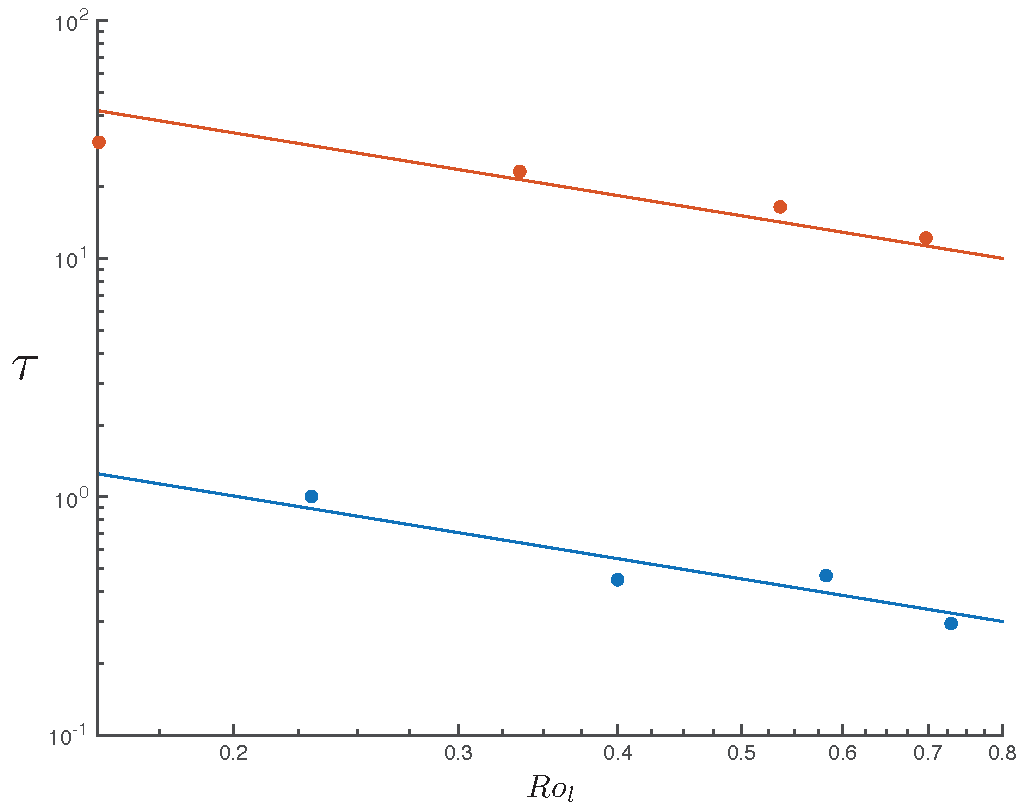
\includegraphics[width=.75\textwidth]{Chapter5/Figures/roltau.pdf}
        \caption{The timescale of core-mantle boundary dipole field variation as a function of local Rossby number for models with (red) and without (blue) a solid Fe-S mantle layer. The solid lines are best fit lines $\tau \propto  Ro_{l}^{-.875}$.}
        \label{fig:tauscale}
\end{figure}

\subsection{Magnetic Field}
\subsubsection{Gauss Coefficients and Locals Rossby Number}
The main observable we have to compare dynamo models of Mercury's magnetic field to the planet Mercury are the Gauss coefficients obtained from an analysis of the MESSENGER and Mariner 10 magnetometer data. Primarily, we we will compare the $g_1^0$ and $g_2^0$ Gauss coefficients which have been observed to be $190\pm14 \textrm{nT}$ and $74\pm \textrm{nT}$ respectively (see chapter \ref{chap:doublesnowstates} for more information on the observations of Mercury's magnetic field).

The strength of the $g_1^0$ and $g_2^0$ Gauss coefficients for each model is displayed in table \ref{tab:fesresults}. For the $I_{\#}$ models, the field is multipolar and small scale so the $g_1^0$ and $g_2^0$ components are quite small ($\mathcal{O}\left(10^{3}\right) nT$ and $\mathcal{O}\left(10^{2}\right) nT$ respectively). This is a key component of the model of \citet{christensen06}, the higher multipole are preferentially attenuated by the thick, stably stratified region above the convecting part of the core.

For the models which possess a solid, conducting mantle layer, the observed Gauss coefficients are far too strong to be compatible with Mercury's magnetic field. The $g_1^0$ coefficient is $\mathcal{O}\left(10^5\right) \textrm{nT}$ for all models, which is three orders of magnitude larger than the $g_1^0$ observed at Mercury. Also the $g_2^0$ component is two orders of magnitude too large and possesses the opposite sign as $g_1^0$. Both of these properties make the $g_2^0$ component incompatible with Mercury's observed magnetic field.

The addition of an electrically conducting mantle layer has a modest effect on the local Rossby number. In all models it appears as though the local Rossby number decreases slightly when a solid mantle layer is added (Table \ref{tab:fesresults}), however all remain above the critical value of $Ro_{l}\approx 0.12$. If the scaling of \citet{christensen06scaling} applies, we would predict a multipolar field for all models presented here. This decrease in local Rossby number stems from two competing effects, the addition of a FeS layer increases the predominant length scale of the velocity field ($\ell_u$) while decreasing the Rossby number ($Ro$, see table \ref{tab:fesresults}). Recall from section \ref{sec:rol} that the definition of the local Rossby number is
\begin{equation}
Ro_{l}=Ro\frac{\bar{\ell}_{u}}{\pi}.
\end{equation}
Because models with an FeS layer see their velocity, and hence their Rossby number decrease more than their length scale increases, the local Rossby number decreases when an FeS layer is added.

We can derive some insight into the large $g_1^0$ in the $C_\#$ models by examining the power spectrum (figure \ref{fig:powspec}). In this figure we see that the spectrum for a model without an FeS layer ($I_4$, red) has a range of less than an order of magnitude for the first 10 multipoles, with a peak at $L=3$. This is not surprising, as this model has a local Rossby number greater than $0.12$ and is run under the same parameters as the models that \citet{christensen06scaling} used to derive the local Rossby number.

The power spectrum for a model with a FeS flotation layer ($C_4$, blue) differs considerably from the spectrum of $I_4$. Here we see that the model is predominantly dipolar, as the $L=1$ component is over an order of magnitude stronger than the next strongest component ($L=5$).

The difference in power spectra that we observe in figure \ref{fig:powspec} provides a reason for the difference in $g_1^0$ that we see in table \ref{tab:fesresults}. The addition of an FeS layer has the effect of making the magnetic field much more dipolar than it would be otherwise. Since dipolar fields have $L=1$ they vary much more slowly than fields with higher $L$ so they are not efficiently screened by the solid conducting FeS layer. This results in a strong magnetic field at the surface and a $g_1^0$ component that does not match the observed $g_1^0$ of Mercury. 
\begin{figure}
	\centering
	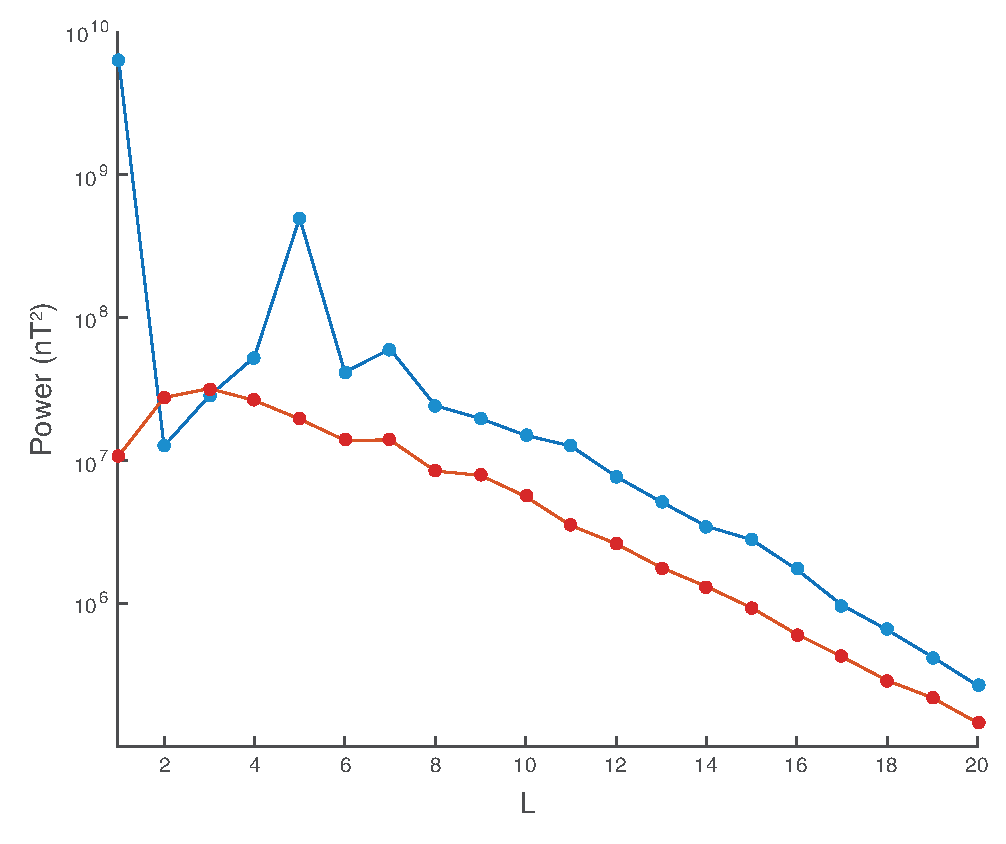
\includegraphics[width=.8\linewidth]{Chapter5/Figures/PowSpec.eps}

        \caption{The temporally averaged surface magnetic power spectrum for model $C_4$ (blue) and model $I_4$ (red). } 
        \label{fig:powspec}
\end{figure}

\subsubsection{Magnetic Field Morphology}
As we expected from the local Rossby number scaling laws, if we plot the radial magnetic field of models without a solid FeS mantle layer, the field morphology is highly non-dipolar and small scale (model $I_4$, figure \ref{fig:nofesbr}).
\begin{figure}
	\centering
        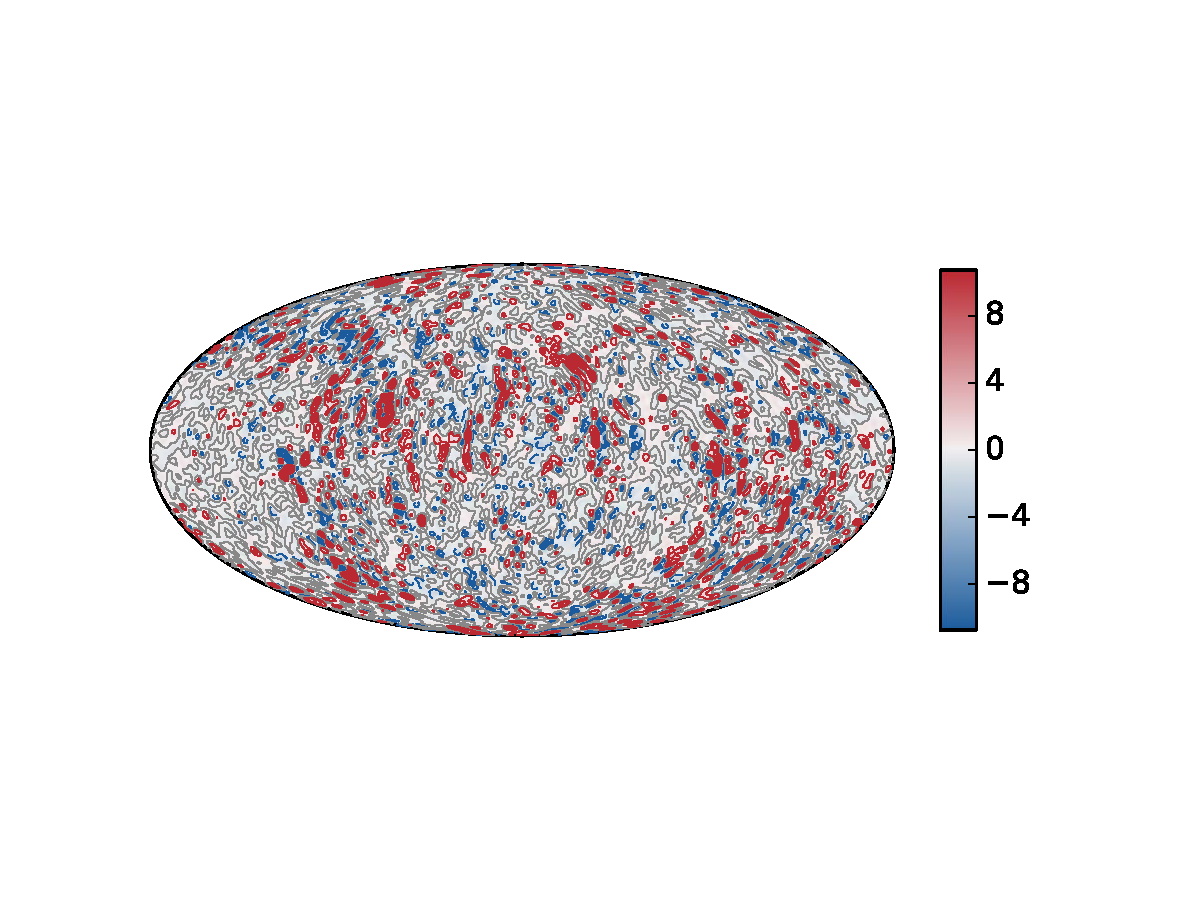
\includegraphics[width=.8\textwidth]{Chapter5/Figures/br10_004_1800_100.pdf} 
        \caption{A snapshot of the radial magnetic field at the core-mantle boundary for model $I_{4}$, units in this figure are non-dimensional.}
        \label{fig:nofesbr}
\end{figure}
The axisymmetric $\phi$ component of the magnetic field also displays very small scale magnetic field with no large scale field at all (model $I_{4}$, figure \ref{fig:nofesbax}). 
\begin{figure}
	\centering
	\begin{subfigure}{.4\textwidth}
		\centering
	        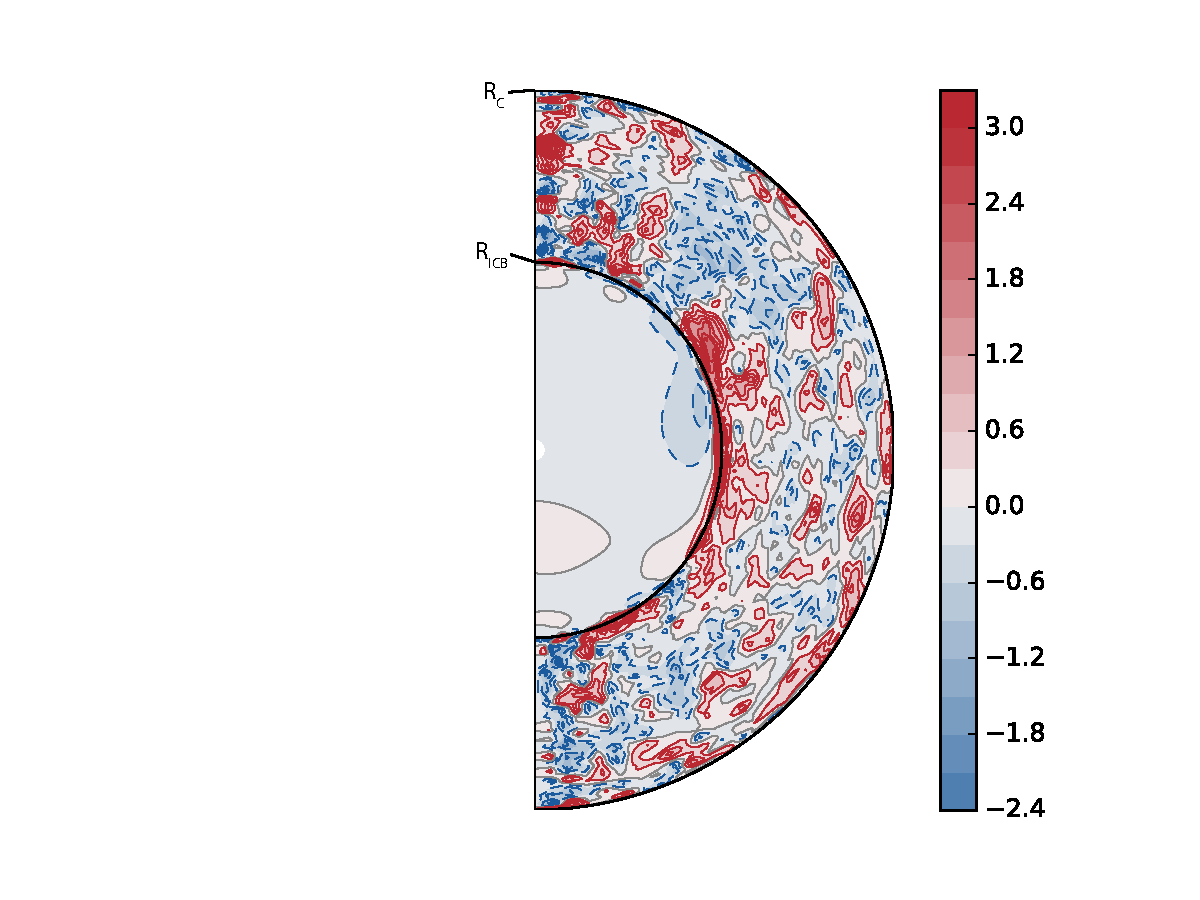
\includegraphics[width=\linewidth]{Chapter5/Figures/btor10_004_1800.pdf}
     		
		\caption{\label{fig:nofesbax}}
        \end{subfigure}%
        \begin{subfigure}{.4\textwidth}
	        \centering
	        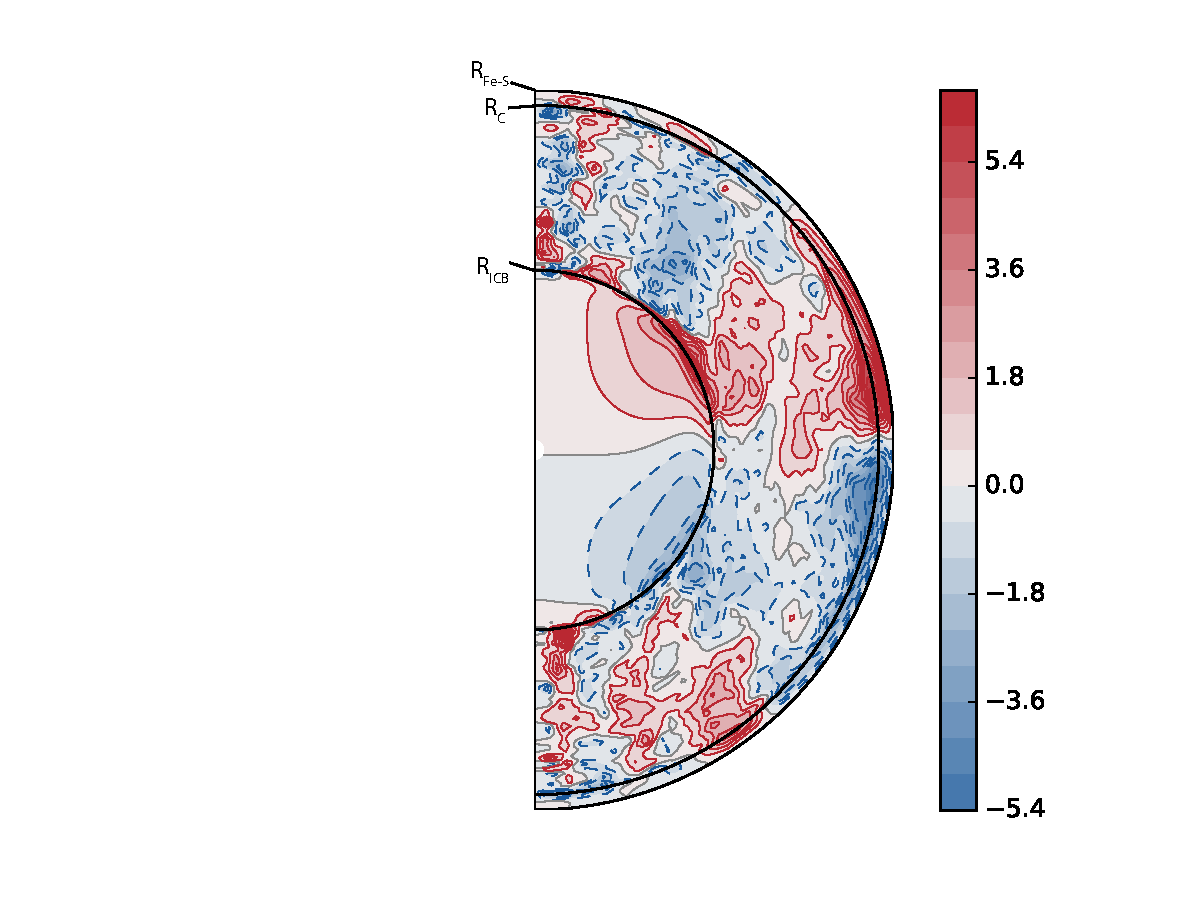
\includegraphics[width=\linewidth]{Chapter5/Figures/btor11_004_1631.pdf}
	       
	        \caption{ \label{fig:fesbax}}
        \end{subfigure}
        \caption{Snapshots of the axisymmetric $\phi$ component of the magnetic field within the core for model $I_{4}$ (\subref{fig:nofesbax}) and model $C_{4}$ (\subref{fig:fesbax}). The region nearest the centre of the semicircle in both figures is the inner core, followed by the fluid outer core (moving outwards) followed by the conducting mantle layer in model $C_4$. Units in these figures are non-dimensional.}
\end{figure}
If we examine the axisymmetric $\phi$ component of the field within the core and conducting layer for a model with an FeS mantle layer (figure \ref{fig:fesbax}), we find very similar results to what we saw in chapter \ref{chap:superearth}. Near the core-mantle boundary very strong axisymmetric $\phi$ field is generated by the shear between the stationary, solid mantle and the strong, large scale zonal flows that exist within the fluid outer core (figure \ref{fig:fesutor})
\begin{figure}
	\centering
        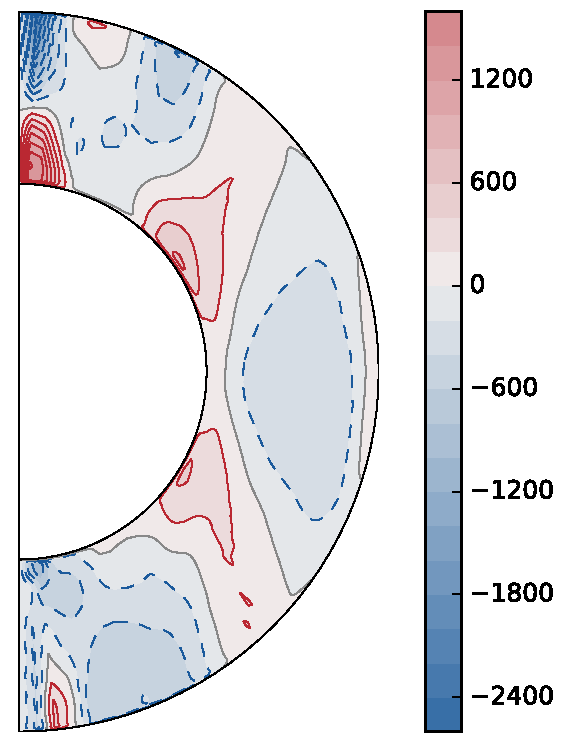
\includegraphics[width=.4\textwidth]{Chapter5/Figures/utor11_001_1100-1330.pdf} 
        \caption{The axisymmetric $\phi$ component of velocity for model $C_1$ average over approximately  $\text{1/2}$ of a magnetic diffusion time.}
        \label{fig:fesutor}
\end{figure}
. There is a stark difference between the axisymmetric $\phi$ field in the case without a solid conducting layer (figure \ref{fig:nofesbax}) and the models with a conducting layer (figure \ref{fig:fesbax}). The magnetic shear at the core-mantle boundary has the effect of dramatically increasing the length scale of the axisymmetric toroidal magnetic field. It also organises the axisymmetric $\phi$ component of the field into a pattern more commonly seen in models with a much lower local Rossby numbers, which generate dipolar magnetic fields (e.g. figure \ref{fig:maggen}a).

This shear of the magnetic field is also evident in plots of the $\phi$ component of the magnetic field at the core-mantle boundary. In figure \ref{fig:nofesbph} we see that without a solid, electrically conducting layer the field is very small scale and disorganised. Once an electrically conducting solid mantle layer is added (figure \ref{fig:fesbph}) the large scale shear imposed by the zonal flows dramatically increases the length scale of the $\phi$ component of the field.
\begin{figure}
	\centering
	\begin{subfigure}{.8\textwidth}
		\centering
	        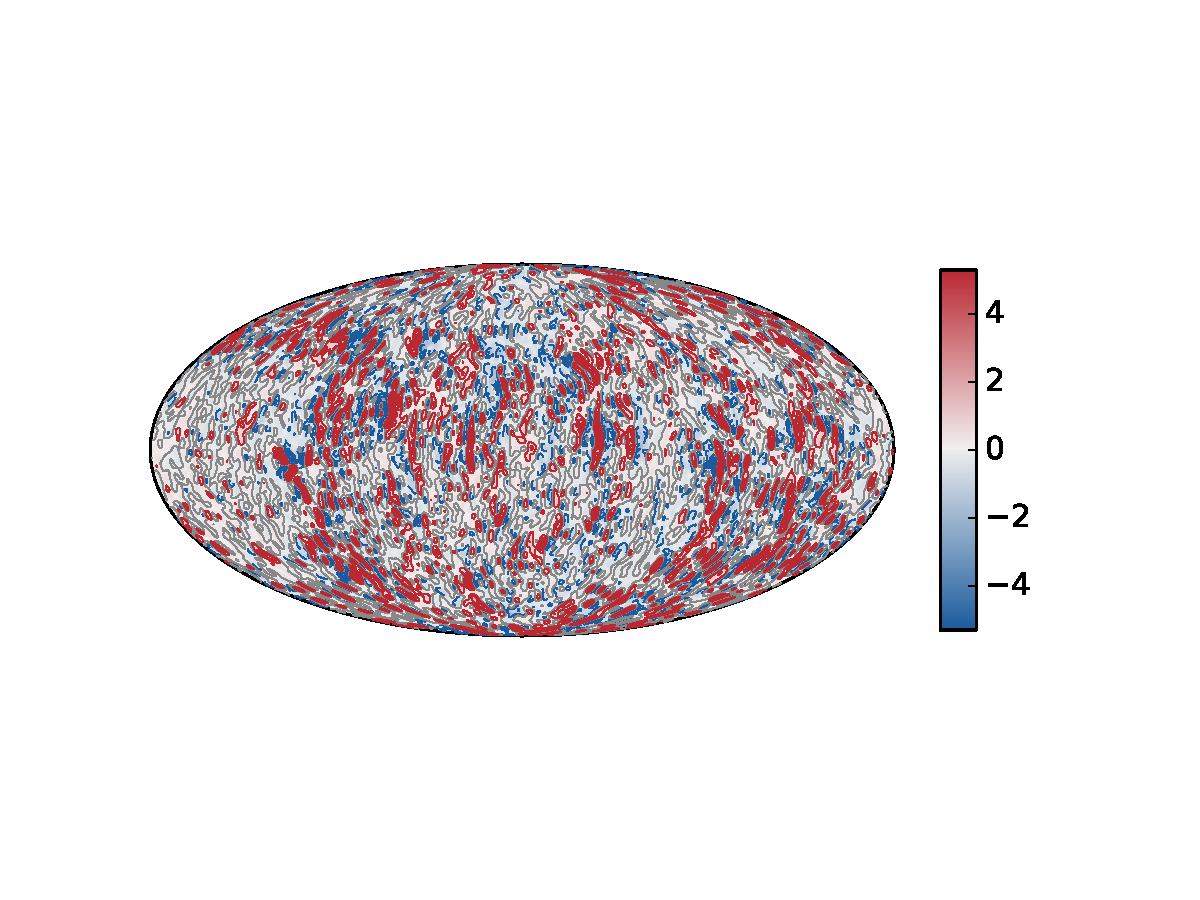
\includegraphics[width=\linewidth]{Chapter5/Figures/bph10_004_1800_100.pdf}
     		
		\caption{\label{fig:nofesbph}}
        \end{subfigure}
        
        \begin{subfigure}{.8\textwidth}
	        \centering
	        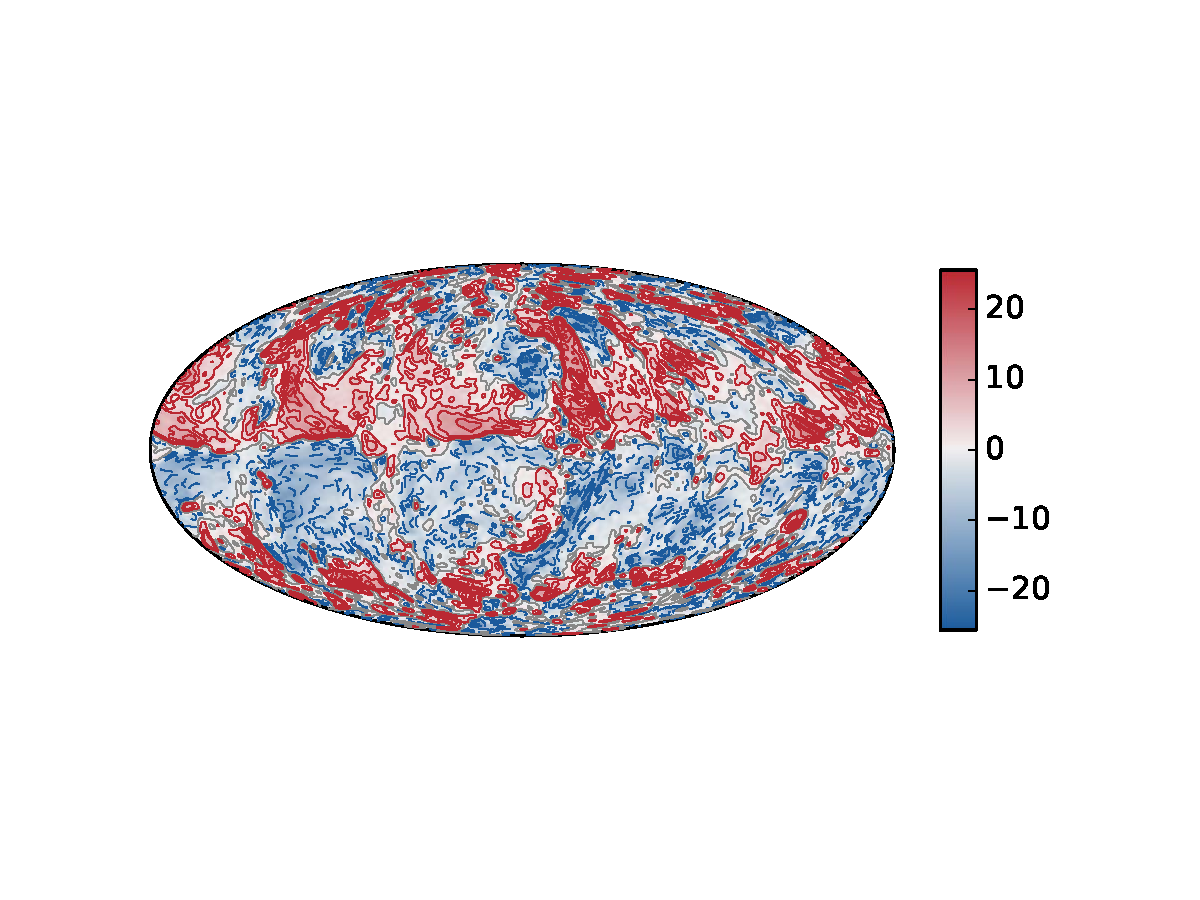
\includegraphics[width=\linewidth]{Chapter5/Figures/bph11_004_1631_100.pdf}
	       
	        \caption{ \label{fig:fesbph}}
        \end{subfigure}
        \caption{Snapshots of the $\phi$ component of the magnetic field at the core-mantle boundary for a model without an FeS layer (\subref{fig:nofesbph}) and with an FeS layer (\subref{fig:fesbph}). Units in these figures are non-dimensional and are from models $I_4$ and $C_4$.} 
        \label{fig:bph}
\end{figure}

This large scale toroidal magnetic field generates a radial magnetic field which is also large scale, and predominantly dipolar (figure \ref{fig:fesbrcmb}). This is a completely different magnetic field morphology compared to the insulating mantle model at the same parameters (figure \ref{fig:fesbrcmb}).
\begin{figure}
	\centering
	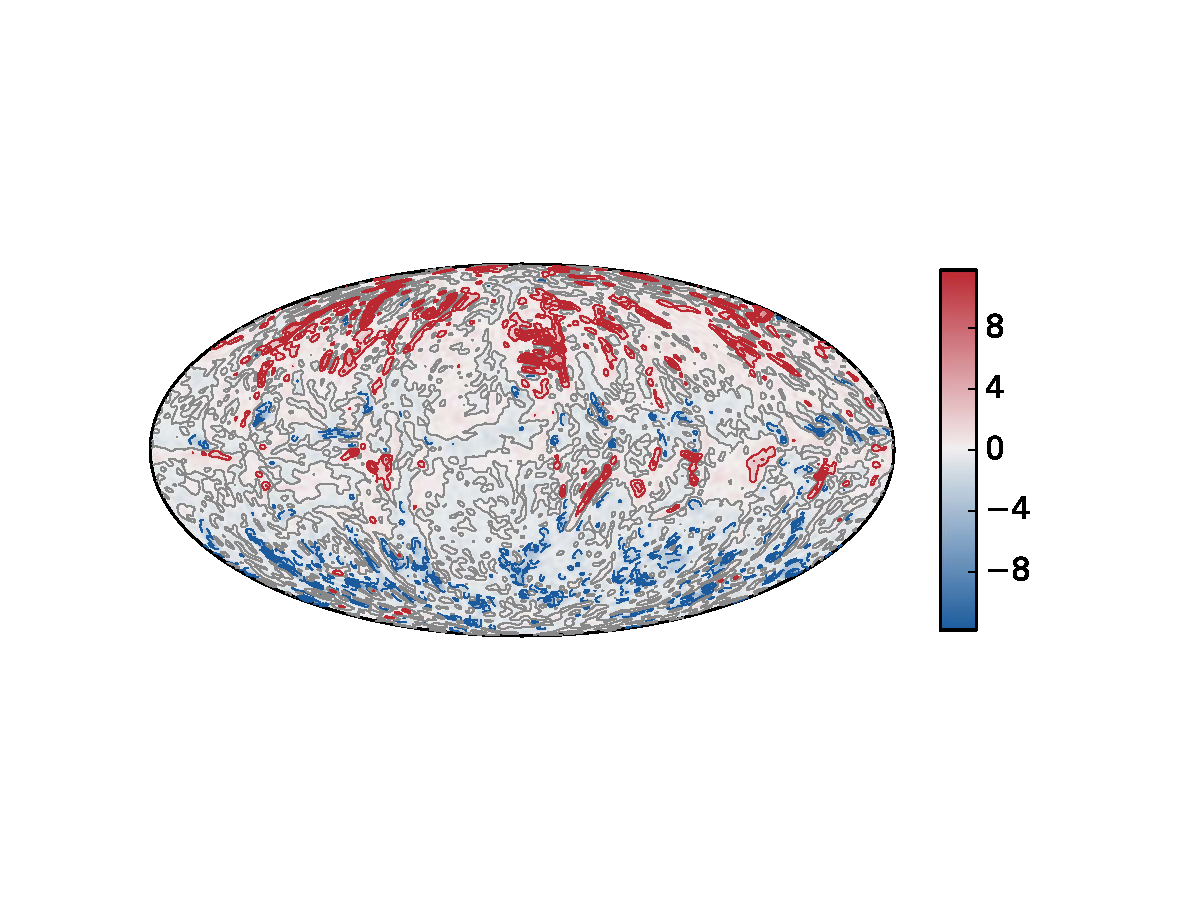
\includegraphics[width=.8\linewidth]{Chapter5/Figures/br11_004_1631_100.pdf}	
	\caption{A snapshot of the radial component of the magnetic field at the core-mantle boundary for model $C_4$. Units in this figure are non-dimensional.}
	\label{fig:fesbrcmb}
\end{figure}
As we discussed in chapter \ref{chap:superearth}, if there is an electrically conducting mantle layer present in the model the radial component of the magnetic field at the core-mantle boundary is modified before it is observed at the surface. The conducting mantle layer will attenuate the field by a factor of $e^{-d\sqrt{\omega/(2 \eta)}}$ (refer to chapter \ref{chap:superearth} for a discussion of this factor). In figure \ref{fig:fesbrddp} we plot the radial component of the magnetic field above the conducting FeS layer we see that the strength of the magnetic field has been reduced somewhat and the length scales have increased.
\begin{figure}
	\centering
	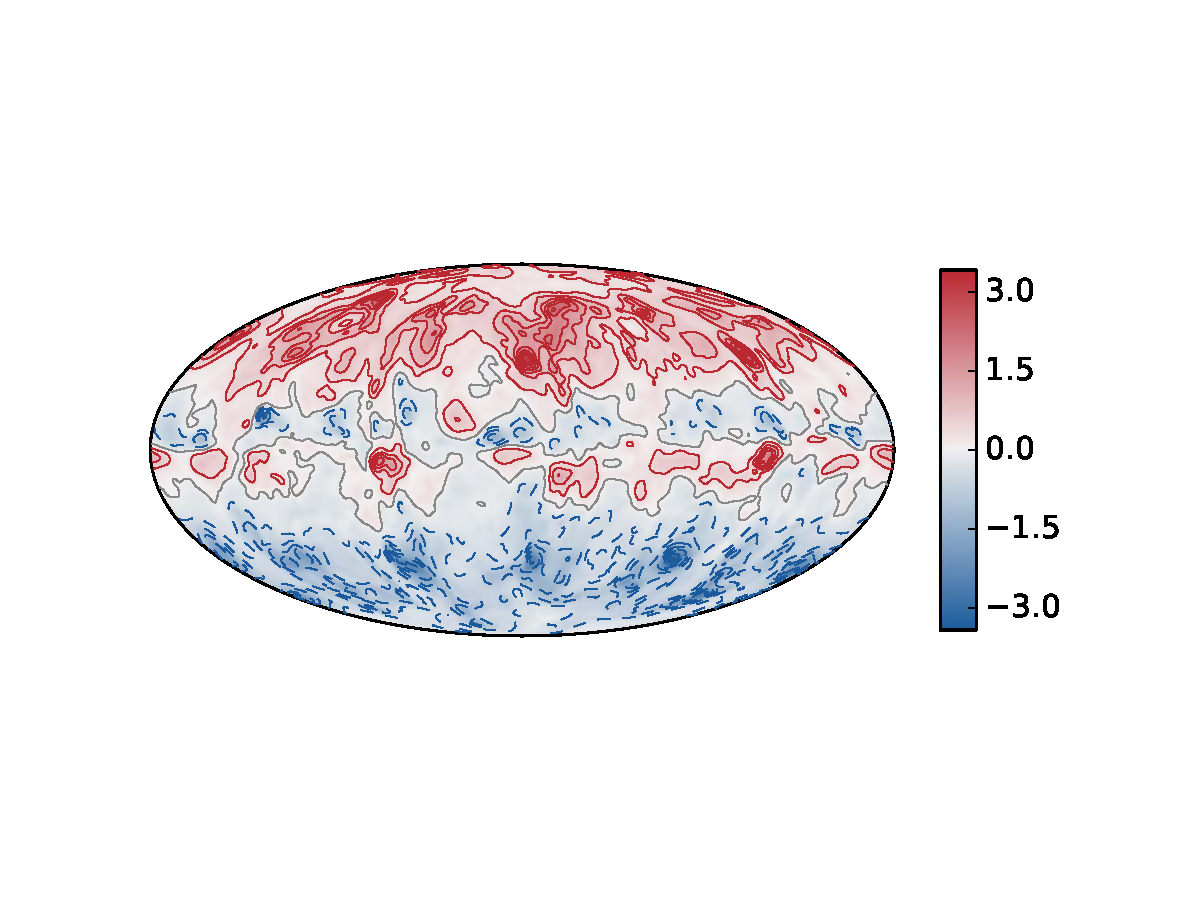
\includegraphics[width=.8\linewidth]{Chapter5/Figures/br11_004_1631_104.pdf}
	\caption{A snapshot of the radial component of the magnetic field at the top of the electrically conducting mantle for model $C_4$. Units in this figure are non-dimensional.}
        \label{fig:fesbrddp}
\end{figure}

Finally, in figure \ref{fig:fessurf} we plot the dimensional radial magnetic field at the surface for model $C_4$. Here it is obvious that this model does not match Mercury's magnetic field at all. The surface fields we observe in figure \ref{fig:fessurf} are several orders of magnitude too large to be consistent with Mercury's magnetic field. Also, we can see that the magnetic equator and the planetary equator appear coincident which is also inconsistent with the observed $400\textrm{km}$ northward shift of Mercury's magnetic equator (figure \ref{fig:Mercurybr}).
\begin{figure}
	\centering
        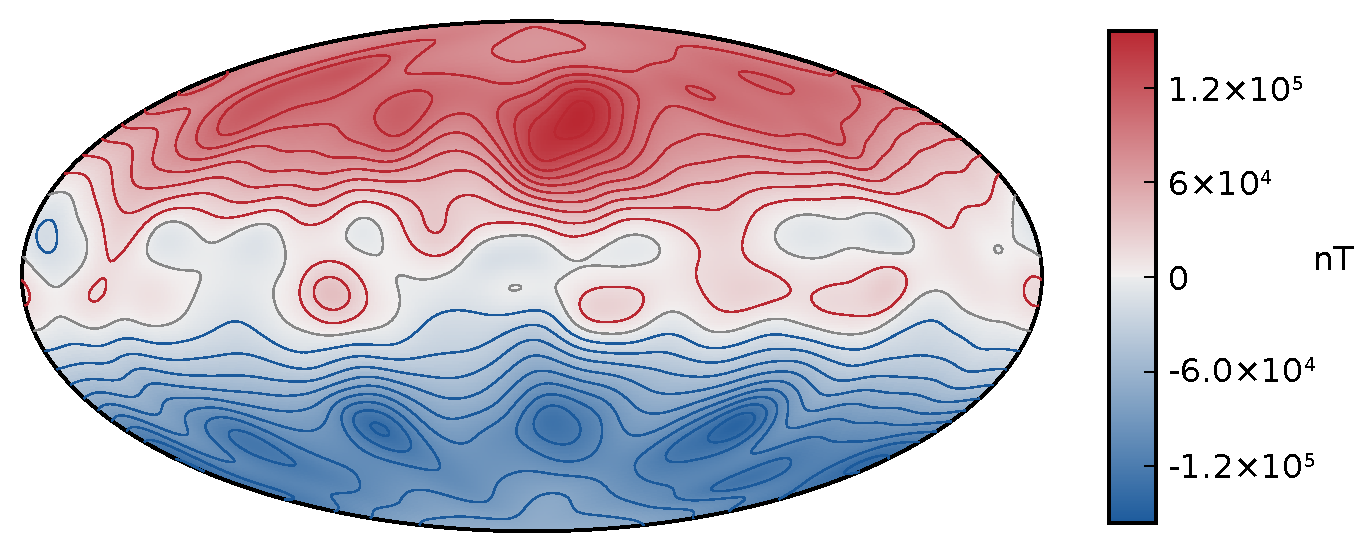
\includegraphics[width=\linewidth]{Chapter5/Figures/br11_004_1631_surf.pdf} 
        \caption{A snapshot of the surface radial magnetic field for model $C_4$ in dimensional units.}
        \label{fig:fessurf}
\end{figure}

In the models presented here we have found that the addition of a solid FeS layer causes the field to become much more dipolar. The reason for this is because of the large scale axisymmetric $\phi$ field sheared out by the zonal flows present in our models. The large scale axisymmetric $\phi$ field that is sheared by these flows is then the seed field for the poloidal field. As large scale seed field tends to create large scale resultant field, the poloidal field from our models is strong and predominantly dipolar.

\section{Conclusion}
We have tested the consequences of a solid, conducting FeS layer on magnetic field generation in Mercury. Models of Mercury's interior have allowed for a deep, dense layer in Mercury's mantle which some studies \citep{smith2012, hauck2013} suggested could explain Mercury's weak axial dipole via the skin effect \citep{christensen06}. We found that when all the consequences of a solid, electrically conducting layer are considered, the addition of a solid FeS layer causes the dynamo to change from generating a multipolar magnetic field to a dipolar field. This strong dipolar field does not vary quickly enough to be effectively screened by the mantle layer, and a magnetic field several orders of magnitude too large to be consistent with Mercury's field is observed at the planetary surface.

This has interesting implications for the scaling laws of \citet{christensen06scaling}. All the models which have a solid conducting mantle layer have a local Rossby number greater than $0.12$, which implies that they should generate a predominantly non-dipolar magnetic field. As we found in this study, while the $\tau-Ro_l$ scaling law appears to apply once an FeS layer is added (figure \ref{fig:tauscale}) the transition point in local Rossby number is not valid in this new geometry. Furthermore, local Rossby number appears to decrease once an electrically conducting mantle layer is added (table \ref{tab:fesresults}) meaning that the scaling law which relates the control parameters to the local Rossby number (equation \ref{eq:rolscaling}) may need to be modified. 

One unresolved question from this study is whether there exists a parameter regime in which the local Rossby number is high enough for a dynamo model with a solid FeS layer to display a multipolar magnetic field. Currently the field is predominantly dipolar because the dynamo is seeded with large scale, dipolar toroidal magnetic field from the shear created between the solid mantle and the zonal flows in the fluid outer core. At high enough buoyancy fluxes (Rossby numbers) the homogenisation of magnetic flux due to convection may outstrip the ability of zonal flows to generate it and a multipolar field could result. As we are unable to run at a local Rossby number that is realistic for Mercury, we do not currently know whether this possible transition is above the local Rossby number that we expect for Mercury ($\mathcal{O}\left(10^1\right)$).
%
%It would seem as though the results that we have found in this chapter contradict the results of chapter \ref{chap:superearth}. In chapter \ref{chap:superearth} we found that the addition of a solid conducting mantle layer made the dynamo less axisymmetric, while in this chapter we found that the addition of a solid conducting mantle layer made the dynamo more dipolar and more axisymmetric. 
%
%A key difference between these two chapters is the parameter regime of the dynamo. In chapter \ref{chap:superearth} the dynamo was chosen to be in a parameter regime of $Ro_{l}<0.12$, meaning that in the absence of a solid conducting mantle layer the dynamo would generate large scale, dipolar fields. In this chapter the parameter regime was chosen so that $Ro_{l}>0.12$ meaning that the generated magnetic field is much smaller scale and non-dipolar.
%
%Common to the models of this section and chapter \ref{chap:superearth} are large scale axisymmetric zonal flows (for example \ref{fig:fesutor}). These flows are caused by a combination of thermal winds and Reynolds stresses and are a common feature of rotating convective systems. In the context of dynamos, they have been studied in detail by \citet{aubert2005zonal}. As we discussed in chapter \ref{chap:superearth}, these zonal flow provide source of shear at the CMB for models with an electrically conducting mantle layer. Poloidal field lines are frozen into the solid immobile mantle and the strong, axisymmetric zonal flows causing a large magnetic shear at the boundary. The effects of this shear are obvious in plots of the axisymmetric toroidal field for  these models (figures \ref{fig:toroidal} and \ref{fig:fesbax}). In these figures large regions of axisymmetric $\phi$ magnetic field are sheared out at the core-mantle boundary by the zonal flows present in both models. 
%
%In the models 

%We can gain some insight into why the models with solid FeS layers generate large scale magnetic fields by considering poloidal magnetic field generation with the Bullard-Gellman formalism (see Appendix \ref{chap:appendix1}) in the scenario where the core has already been seeded with the large scale toroidal field pattern we see in figure \ref{fig:fesbax}. For this scenario we focus on the generation of poloidal field by velocities acting on toroidal fields. These correspond to 
%\begin{equation}
%P_\alpha T_\beta P_\gamma
%\end{equation}
%and
%\begin{equation}
%T_\alpha T_\beta P_\gamma.
%\end{equation}
%Recall that $P$ stands for poloidal and $T$ stands for toroidal, and $\alpha$, $\beta$ and $\gamma$ refer to the velocity field, the seed magnetic field and the resultant magnetic field respectively. We showed in appendix \ref{chap:appendix1} that the latter of these is always zero, but $P_\alpha T_\beta P_\gamma$ requires some analysis.
%
%We see that the toroidal field pattern in figure \ref{fig:fesbph} is predominantly dipolar so we will assign $\beta=1$, $m_\beta=0$ and look at which modes of velocity and magnetic field can make this integral non-zero. The $P_\alpha T_\beta P_\gamma$ integral is an Elsasser type integral, which has its selection rules printed in appendix \ref{chap:appendix1}. For our purposes we are mainly interested in two of these:
%\begin{quote}
%An Elsasser type integral is zero unless:
%\begin{itemize}
%\item $\alpha, \beta, \gamma$ can form the sides of a triangle. This is equivalent to satisfying the triangle inequality: $\left|\alpha-\beta\right|<\gamma<\alpha+\beta$.
%\item One or more of $m_\alpha \pm m_\beta \pm m_\gamma$ is zero.
%\end{itemize}
%\end{quote}
%These two rules constrain the magnitude of $m$ and $L$ of the resultant magnetic field $\gamma$ and velocity field $\alpha$. If $\beta=1$ and $m_\beta=0$ this means that
%\begin{equation}
%\left|\alpha-1\right|<\gamma<\alpha+1
%\end{equation}
%and one or more of 
%\begin{equation}
%m_\alpha \pm  m_\gamma  = \pm1.
%\end{equation}
%These equations show that $\alpha \approx \gamma$ and $m_\alpha \approx m_\gamma$
%!TEX root = ../thesis.tex

\chapter{Conclusions and Future Work}
\label{chap:conclusion}
In this work we have discussed how novel material properties can affect magnetic field generation in planets. We have focussed on the magnetic fields of the planet Mercury, as well as the magnetic fields of terrestrial planets in other planetary systems. This work has provided predictions about the likelihood of detecting exoplanetary magnetic fields (chapter \ref{chap:superearth}). We have also discussed a new model to explain the weak dipolar field measured at Mercury (chapter \ref{chap:doublesnowstates}). Finally, we tested a second model which was proposed \citep{smith2012, hauck2013} to explain Mercury's weak magnetic field (chapter \ref{chap:floatationlayers}) and found that the magnetic fields it produced did not match those measured at Mercury.

\subsection{The Magnetic Fields of Exoplanets with Metallized Mantles}
In chapter \ref{chap:superearth} we used recent evidence which indicates that the materials which commonly comprise the mantles of terrestrial planets can metallise and conduct electricity under mantle conditions \citep{nellis2010, tsuchiya2011, ohta2012}. We found that magnetic field generated by the core dynamo would become simultaneously trapped in the solid, immobile mantle and the strong, axisymmetric zonal flows of the core. This leads to a strong axisymmetric toroidal field within the core by magnetic stretching at the core-mantle boundary. This toroidal field can only be converted to a non-axisymmetric poloidal field, due to geometrical constraints which become apparent by applying the Bullard-Gelman formalism to this scenario (Appendix \ref{chap:appendix1}). This non-axisymmetric poloidal field appears as a time varying flow when it is advected by the zonal flows in the core, and is attenuated by the screening effect of the electrically conducting mantle. We found that this means a exoplanet with a solid, electrically conducting mantle may have a weak observed magnetic field despite having a much stronger internal magnetic field. The results from this study are published in \citet{vilim2013}.
 
\subsection{The Magnetic Field of Mercury}
In this work we discussed two possible ways of generating Mercury's weak, equatorially asymmetric magnetic field. The first appealed to a ``double snow state'', a unique core solidification regime which Mercury may occupy due to a combination of its core-composition and the pressures found within it. In this scenario iron freezes first part way through the liquid outer core and injects buoyancy there. We modelled this as a stably stratified layer and found that this split the core into two dynamo generation regions which generated magnetic field of opposite polarity. These magnetic fields superposed to create a weak, dipolar magnetic field. We also found that the magnetic field generated by these models did not match the recently northward displacement of Mercury's magnetic equator \citep{smith2012}. The results form this study are published in \citet{vilim2010}

In this work we also tested a recently proposed model of Mercury's interior. This model proposed a layer of FeS at the top of Mercury's core which would preferentially attenuate the non-dipolar components of the generated magnetic field. It was proposed that this could explain the moment of inertia of Mercury' outer shell and its weak observed magnetic field. We found that the addition of a solid, electrically conducting layer at the top of the core caused significant Lorentz stretching there, which lead to a strong, dipolar magnetic field and a decrease in the characteristic timescale of the dynamo. This means that a solid electrically conducting layer which is thin enough to be consistent with the moment of inertia observations is insufficiently thin to screen the magnetic field effectively, leading to a strong, dipolar observed magnetic field.


\subsection{Future Work}
There are several avenues which should be explored as extensions to the work presented in this thesis.

\subsubsection{Metallized Mantles at High Local Rossby Numbers}
In chapter \ref{chap:superearth} we only focussed on dynamo models with $Ro_l<0.12$, which means that these dynamos would be predominantly dipolar in the absence of a metallised mantle layer. While there are almost certainly exoplanets with $Ro_l>0.12$, an analysis of these models was outside the scope of the work in chapter \ref{chap:superearth}. If $Ro_l>0.12$ the scaling laws of \citet{christensen06scaling} would predict that these dynamos should generate multipolar magnetic fields. Since mode $l$ will decay in field strength from the core as $\left(a/r\right)^{l+2}$ the strongest components of these dynamos would decay in strength very rapidly with distance and should be much more difficult to detect. 

When testing the feasibility of a solid, electrically conducting layer at the bottom of Mercury's mantle (chapter \ref{chap:floatationlayers}) we discovered that at high local Rossby numbers an electrically conducting mantle changed the resultant magnetic field from being small scale and highly time variable to large scale and predominantly dipolar. As we discussed in chapter \ref{chap:floatationlayers} this was because the electrically conducting mantle provides a source of shear, which promotes the generation of large scale, dipolar toroidal field. This toroidal field is then converted into large scale dipolar poloidal field leading to a strong dipolar magnetic field. 

This means that contrary to the conclusions of chapter \ref{chap:superearth}, a metallized mantle layer may make some dynamos easier to detect rather than more difficult as we concluded. In order to determine whether this assessment is true, we plan to re-analyse our current results in the context of exoplanets.

\subsubsection{Matching $g_1^1$ in Double Snow State Models}
All of the results presented in chapter \ref{chap:doublesnowstates} were finished before the publication of the $g_2^0$ obtained by the MESSENGER spacecraft \citep{anderson2012}. While these results currently do not match the $g_1^1$ component, it is not known whether a double snow state model running with different parameters or in a different geometry could match the $g_1^1$ component. In future work we will run numerical dynamo models to attempt to match a model with a double snow state to the newest MESSENGER observations.
%!TEX root = ../thesis.tex
\appendix
\chapter{The Bullard-Gellman Formalism}
\label{chap:appendix1}
One important way of understanding how dynamos operate is called the Bullard-Gellman formalism  \citep{bullard1954}. This simplified framework was developed to study how interactions between fluid motion and seed magnetic fields can generate new magnetic fields. While a detailed derivation of this formalism is outside the scope of this work (see \citet{bullard1954}) we will introduce the basic derivation here, which will allow us to interpret the results of chapter \ref{chap:superearth}.

The Bullard-Gellman formalism begins with the assumption of an incompressible fluid in a sphere of non-dimensional radius 1 and seeks to find solutions to the equations
\begin{align}
\frac{\partial \mbf{B}}{\partial t}&=\nabla\times\left(\mbf{u}\times\mbf{B}\right)+\eta\nabla^{2}\mbf{B} & \textrm{for } r<1
\end{align}
of the form
\begin{equation}
\mbf{B}\left(\mbf{r},t\right)=\mbf{B}\left(\mbf{r}\right)e^{\lambda t}.
\end{equation}
Substituting this into this into the magnetic induction equation means we seek to find solutions to 
\begin{equation}
\left(\lambda-\nabla^{2}\right)\mbf{B}=\nabla\times\left(\mbf{u}\times\mbf{B}\right)\label{eq:bgmie}.
\end{equation}
Using the Toroidal-Poloidal expansion (equation \ref{eq:toroidalpoloidal}\footnote{This expansion differs in form from the expansion we saw in equation \ref{eq:laplaceexpansion}. In this case $A_{l}^{m}$ can be complex which will make the subsequent expressions simpler.}) along with the spherical harmonic expansion
\begin{equation}
A=\sum_{l=1}^{\infty}\sum_{m=0}^{l}A_{l}^{m}Y_{l}^{m}\left(\theta,\phi\right)
\end{equation}
on the magnetic field and velocity field to give
\begin{align}
\mbf{B}=\mbf{B}_{T}+\mbf{B}_{P}=\sum_{L=1}^{\infty}\sum_{m=0}^{L} \left(\mbf{T}_{l}^{m}+\mbf{P}_{l}^{m}\right) \\
\mbf{u}=\mbf{u}_{T}+\mbf{u}_{P}=\sum_{L=1}^{\infty}\sum_{m=0}^{L} \left(\mbf{t}_{l}^{m}+\mbf{p}_{l}^{m}\right).
\end{align}
Here we have denoted a single component of the magnetic field in capital letters (e.g. $\mbf{T}_{l}^{m}$) and a single component of the velocity field in lower case letters (e.g. $\mbf{t}_{l}^{m}$). Following the definition of equation \ref{eq:toroidalpoloidal} we can write
\begin{align}
\mbf{T}_l^m &= \nabla \times \left[T_l^m\left(r\right) Y_l^m \left(\theta, \phi\right) \hat{r}\right] \label{eq:Texpansion}\\ 
\mbf{P}_l^m &= \nabla \times \nabla \times \left[P_l^m\left(r\right) Y_l^m \left(\theta, \phi\right) \hat{r}\right]\label{eq:Pexpansion} \\
\mbf{t}_l^m &= \nabla \times \left[t_l^m\left(r\right) Y_l^m \left(\theta, \phi\right)\hat{r}\right] \label{eq:texpansion}\\
\mbf{p}_l^m &= \nabla \times \nabla \times \left[p_l^m\left(r\right) Y_l^m \left(\theta, \phi\right) \hat{r}\right].\label{eq:pexpansion}
\end{align}
If we substitute equations \ref{eq:Texpansion}-\ref{eq:pexpansion} into \ref{eq:bgmie} we get
\begin{equation}
 (\lambda-\nabla^2) \left[\sum_1 \left(\mbf{T}_{l_1}^{m_1} + \mbf{P}_{l_1}^{m_1}\right)\right]
  = \nabla \times \left[\sum_2 \left(\mbf{t}_{l_2}^{m_2} +
  \mbf{p}_{l_2}^{m_2}\right)\right] \times \left[\sum_3 \left(\mbf{T}_{l_3}^{m_3} +
  \mbf{P}_{l_3}^{m_3}\right)\right] \label{eq:bgexpand1}
\end{equation}
where the subscripts under the sums indicate that we sum over the $l$ and $m$ of that index. This expression gives a sum over resultant magnetic field components (subscript $1$) produced by all velocity modes (subscript $2$) acting on all magnetic field modes (subscript $3$). In order to get interpretable predictions, we would like to know the growth rate of one mode (one $l_1$, $m_1$ combination) due to specific velocity and magnetic field modes. To get this, we will take the inner product of equation \ref{eq:bgexpand1} with a single toroidal or poloidal mode which are defined as:
\begin{align}
\left[\nabla\times\left(Y_{l_1}^{m_1}\right)\hat{r}\right]^{*}\\
\left[\nabla\times\nabla\times\left(Y_{l_1}^{m_1}\right)\hat{r}\right]^{*}
\end{align}
respectively, giving
\begin{multline}
\oint_S \left[\nabla \times (Y_{l_1}^{m_1}(\theta,\phi)\hat{r})\right]^* \cdot (\lambda-\nabla^2)  \left[\sum_1
      \left(\mbf{T}_{l_1}^{m_1} + \mbf{P}_{l_1}^{m_1}\right)\right] dS = \\
 \oint_S \left[\nabla \times(Y_{l_1}^{m_1}(\theta,\phi)\hat{r})\right]^* \cdot \nabla \times \left[\sum_2 \left(\mbf{t}_{l_2}^{m_2} +
  \mbf{p}_{l_2}^{m_2}\right)\right] \times \left[\sum_3
\left(\mbf{T}_{l_3}^{m_3} + \mbf{P}_{l_3}^{m_3}\right)\right] dS \label{eq:bgtorexpand2}
\end{multline}
and
\begin{multline}
\oint_S \left[\nabla \times \nabla \times (Y_{l_1}^{m_1}(\theta,\phi)\hat{r})\right]^* \cdot (\lambda-\nabla^2)  \left[\sum_1
      \left(\mbf{T}_{l_1}^{m_1} + \mbf{P}_{l_1}^{m_1}\right)\right] dS = \\
 \oint_S \left[\nabla \times \nabla \times(Y_{l_1}^{m_1}(\theta,\phi)\hat{r})\right]^* \cdot \nabla \times \left[\sum_2 \left(\mbf{t}_{l_2}^{m_2} +
  \mbf{p}_{l_2}^{m_2}\right)\right] \times \left[\sum_3
\left(\mbf{T}_{l_3}^{m_3} + \mbf{P}_{l_3}^{m_3}\right)\right] dS.\label{eq:bgpolexpand2}
\end{multline}
Using the orthonormality properties of our toroidal and poloidal fields, as well as the identity
\begin{equation}
\nabla^{2}Y_{l}^{m}=\left[\frac{1}{r^2}\frac{\partial}{\partial r}\left(r^{2}\frac{\partial}{\partial r}\right)-\frac{l\left(l+1\right)}{r^2}\right]Y_{l}^{m}
\end{equation}
i.e. that spherical harmonics are eigenvectors of the angular part of the Laplacian, and the following identities concerning our toroidal and poloidal fields:
\begin{align}
\mbf{T}_{l}^{m}&=\nabla\times\left(T_{l}^{m}\left(r\right)Y_{l}^{m}\left(\theta,\phi\right)\hat{r}\right)=T_{l}^{m}\left(r\right)\nabla\times\left(Y_{l}^{m}\left(\theta,\phi\right)\hat{r}\right)\\
\mbf{P}_{l}^{m}&=\nabla\times\nabla\times\left(P_{l}^{m}\left(r\right)Y_{l}^{m}\left(\theta,\phi\right)\hat{r}\right)=P_{l}^{m}\left(r\right)\nabla\times\left(Y_{l}^{m}\left(\theta,\phi\right)\hat{r}\right)\\
\mbf{t}_{l}^{m}&=\nabla\times\left(t_{l}^{m}\left(r\right)Y_{l}^{m}\left(\theta,\phi\right)\hat{r}\right)=t_{l}^{m}\left(r\right)\nabla\times\nabla\times\left(Y_{l}^{m}\left(\theta,\phi\right)\hat{r}\right)\\
\mbf{p}_{l}^{m}&=\nabla\times\nabla\times\left(p_{l}^{m}\left(r\right)Y_{l}^{m}\left(\theta,\phi\right)\hat{r}\right)=p_{l}^{m}\left(r\right)\nabla\times\nabla\times\left(Y_{l}^{m}\left(\theta,\phi\right)\hat{r}\right)
\end{align}
we can write equations \ref{eq:bgtorexpand2} and \ref{eq:bgpolexpand2} as 
\begin{multline}
\left(\lambda-\nabla^{2}\right)T_{l_1}^{m_1}\left(r\right)=\sum_{1}\sum_{2}
%
t_{l_2}^{m_2} T_{l_3}^{m_3} \oint_S \left[\nabla \times (Y_{l_1}^{m_1}(\theta,\phi)\hat{r})\right]^* \cdot 
\left[\nabla\times\left\{ \left(\nabla\times Y_{l_2}^{m_2}\hat{r}\right)\times \left(\nabla\times Y_{l_3}^{m_3}\hat{r}\right)   \right\}\right]  \\
+
p_{l_2}^{m_2} T_{l_3}^{m_3} \oint_S  \left[\nabla \times (Y_{l_1}^{m_1}(\theta,\phi)\hat{r})\right]^* \cdot
\left[\nabla\times\left\{ \left(\nabla\times\nabla\times Y_{l_2}^{m_2}\hat{r}\right)\times \left(\nabla\times Y_{l_3}^{m_3}\hat{r}\right)   \right\}\right]\\
+
t_{l_2}^{m_2} P_{l_3}^{m_3} \oint_S  \left[\nabla \times (Y_{l_1}^{m_1}(\theta,\phi)\hat{r})\right]^* \cdot 
\left[\nabla\times\left\{ \left(\nabla\times Y_{l_2}^{m_2}\hat{r}\right)\times \left(\nabla\times\nabla\times Y_{l_3}^{m_3}\hat{r}\right)   \right\}\right]  \\
+
p_{l_2}^{m_2} P_{l_3}^{m_3} \oint_S  \left[\nabla \times (Y_{l_1}^{m_1}(\theta,\phi)\hat{r})\right]^* \cdot
\left[\nabla\times\left\{ \left(\nabla\times\nabla\times Y_{l_2}^{m_2}\hat{r}\right)\times \left(\nabla\times\nabla\times Y_{l_3}^{m_3}\hat{r}\right)   \right\}\right]
\label{eq:bgtorexpand3}
\end{multline}
and 
\begin{multline}
\left(\lambda-\nabla^{2}\right)P_{l_1}^{m_1}\left(r\right)=\sum_{1}\sum_{2}
%
 t_{l_2}^{m_2} T_{l_3}^{m_3} \oint_S\left[\nabla\times \nabla \times (Y_{l_1}^{m_1}(\theta,\phi)\hat{r})\right]^* \cdot 
\left[\nabla\times\left\{ \left(\nabla\times Y_{l_2}^{m_2}\hat{r}\right)\times \left(\nabla\times Y_{l_3}^{m_3}\hat{r}\right)   \right\}\right]  \\
+
p_{l_2}^{m_2} T_{l_3}^{m_3} \oint_S  \left[\nabla\times\nabla \times (Y_{l_1}^{m_1}(\theta,\phi)\hat{r})\right]^* \cdot
\left[\nabla\times\left\{ \left(\nabla\times\nabla\times Y_{l_2}^{m_2}\hat{r}\right)\times \left(\nabla\times Y_{l_3}^{m_3}\hat{r}\right)   \right\}\right]\\
+
t_{l_2}^{m_2} P_{l_3}^{m_3} \oint_S  \left[\nabla\times\nabla \times (Y_{l_1}^{m_1}(\theta,\phi)\hat{r})\right]^* \cdot 
\left[\nabla\times\left\{ \left(\nabla\times Y_{l_2}^{m_2}\hat{r}\right)\times \left(\nabla\times\nabla\times Y_{l_3}^{m_3}\hat{r}\right)   \right\}\right]  \\
+
p_{l_2}^{m_2} P_{l_3}^{m_3} \oint_S \left[\nabla\times\nabla \times (Y_{l_1}^{m_1}(\theta,\phi)\hat{r})\right]^* \cdot
\left[\nabla\times\left\{ \left(\nabla\times\nabla\times Y_{l_2}^{m_2}\hat{r}\right)\times \left(\nabla\times\nabla\times Y_{l_3}^{m_3}\hat{r}\right)   \right\}\right].
\label{eq:bgpolexpand3}
\end{multline}
All of the integrals in equations \ref{eq:bgtorexpand3} and \ref{eq:bgpolexpand3} can be represented as an integral of the form
\begin{equation}
G = \oint_S Y_{l_1}^{m_1*}Y_{l_2}^{m_2}Y_{l_3}^{m_3} dS \label{eq:adamsgaunt}
\end{equation}
or
\begin{equation}
L = \oint_S Y_{l_1}^{m_1*}\left(\frac{\partial
        Y_{l_2}^{m_2}}{\partial \theta}\frac{\partial
        Y_{l_3}^{m_3}}{\partial \phi} - \frac{\partial
        Y_{l_2}^{m_2}}{\partial \phi}\frac{\partial
        Y_{l_3}^{m_3}}{\partial \theta}\right) dS. \label{eq:elsasser}
\end{equation}
Integrals of the form in equation \ref{eq:adamsgaunt} are known as Adams-Gaunt integrals, and integrals of the form in equation \ref{eq:elsasser} are known as Elsasser integrals. For simplicity, and historical reasons we will introduce some notation to simplify equations \ref{eq:bgtorexpand3} and \ref{eq:bgpolexpand3}. We will say the spherical harmonic index of the magnetic field being created is $\gamma$, the velocity field will have index $\alpha$ and the seed magnetic field will have index $\beta$. Furthermore, we will represent terms involving a poloidal field (e.g. $\nabla\times\nabla\times Y_{l_2}^{m_2}\hat{r}$) as $P$ and terms representing a toroidal field (e.g. $\nabla\times Y_{l_2}^{m_2}\hat{r}$) as $T$. For example, we could then represent the integral
\begin{equation}
p_{l_2}^{m_2} P_{l_3}^{m_3} \oint_S \left[\nabla\times\nabla \times (Y_{l_1}^{m_1}(\theta,\phi)\hat{r})\right]^* \cdot
\left[\nabla\times\left\{ \left(\nabla\times\nabla\times Y_{l_2}^{m_2}\hat{r}\right)\times \left(\nabla\times\nabla\times Y_{l_3}^{m_3}\hat{r}\right)   \right\}\right]
\end{equation}
as $P_{\alpha}P_{\beta}P_{\gamma}$. If we wish to refer to the order of the spherical harmonic we will refer to it as $m_\gamma$, $m_\alpha$, or $m_\beta$. Under this notation equations  \ref{eq:bgtorexpand3} and \ref{eq:bgpolexpand3} can be represented as 
\begin{equation}
\left(\lambda-\nabla^{2}\right)T_{\gamma}\left(r\right)=\sum_{\alpha,\beta}\left(T_\alpha T_\beta T_\gamma +P_\alpha T_\beta T_\gamma+T_\alpha P_\beta T_\gamma+P_\alpha P_\beta T_\gamma\right)\label{eq:bgtorexpand4}
\end{equation}
and 
\begin{equation}
\left(\lambda-\nabla^{2}\right)P_{\gamma}\left(r\right)=\sum_{\alpha,\beta}\left(T_\alpha T_\beta P_\gamma +P_\alpha T_\beta P_\gamma+T_\alpha P_\beta P_\gamma+P_\alpha P_\beta P_\gamma\right).\label{eq:bgpolexpand4}
\end{equation}
The Adams-Gaunt types integral are 
\begin{align}
P_\alpha P_\beta P_\gamma \\
T_\alpha P_\beta T_\gamma \\
P_\alpha T_\beta T_\gamma,
\end{align}
the Elsasser type integrals are
\begin{align}
T_\alpha P_\beta P_\gamma \\
P_\alpha T_\beta P_\gamma \\
P_\alpha P_\beta T_\gamma \\
T_\alpha T_\beta T_\gamma
\end{align}
while integrals of the form $T_\alpha T_\beta P_\gamma$ are always zero.

Equations \ref{eq:bgtorexpand4} and \ref{eq:bgpolexpand4} have a straightforward interpretation, in order for a given magnetic field mode ($\gamma$) to grow, the right hand sides of these equations must be greater than zero. This requires the evaluation of the integrals in these equations. The integrals in  \ref{eq:bgtorexpand4} and \ref{eq:bgpolexpand4} are zero in many cases, the instances where they are \emph{not} are defined by selection rules. For the Adams-Gaunt type, the integral is zero unless:
\begin{itemize}
\item $\alpha+\beta+\gamma$ is even.
\item $\alpha, \beta, \gamma$ can form the sides of a triangle. This is equivalent to satisfying the triangle inequality: $\left|\alpha-\beta\right|<\gamma<\alpha+\beta$.
\item One or more of $m_\alpha \pm m_\beta \pm m_\gamma$ is zero.
\item Either three or one of the harmonics has a $\cos\left(m\phi\right)$ term, with $m=0$ counting as a $\cos\left(m\phi\right)$.
\end{itemize}
Elsasser integrals are zero unless:
\begin{itemize}
\item $\alpha+\beta+\gamma$ is odd.
\item $\alpha, \beta, \gamma$ can form the sides of a triangle. This is equivalent to satisfying the triangle inequality: $\left|\alpha-\beta\right|<\gamma<\alpha+\beta$.
\item One or more of $m_\alpha \pm m_\beta \pm m_\gamma$ is zero.
\item Either two or none of the harmonics has a $\cos\left(m\phi\right)$ term, with $m=0$ counting as a $\cos\left(m\phi\right)$.
\item No two harmonics are identical.
\end{itemize}
It is important to note that the only way a magnetic field can be maintained in this framework is if there is a way for magnetic energy induced from a mode ($\beta$) to eventually be fed back into that mode. If this does not take place, the energy supplied by $\mbf{u}$ in mode $\alpha$ will be dissipated over infinitely many magnetic field modes and diffused away at small scale.

A useful tool to visualise how magnetic fields are generated in this framework is an \emph{interaction diagram}. In an interaction diagram the dynamo process is represented as a directed graph with vertices forming magnetic field nodes (which can be induced or seed fields) and vertices representing the velocity field modes. 

For example, one finite interaction diagram occurs when $P_1^0$ ($\beta=1$, $m_\beta=0$) is acted on by $T_1^0$ ($\alpha=1$, $m_\alpha=0$) to produce $T_2^0$ ($\gamma=2$, $m_\gamma=0$). This would be represented in an interaction diagram as figure \ref{fig:interaction-differentialrotation}.
\begin{figure}
	\centering
	\noindent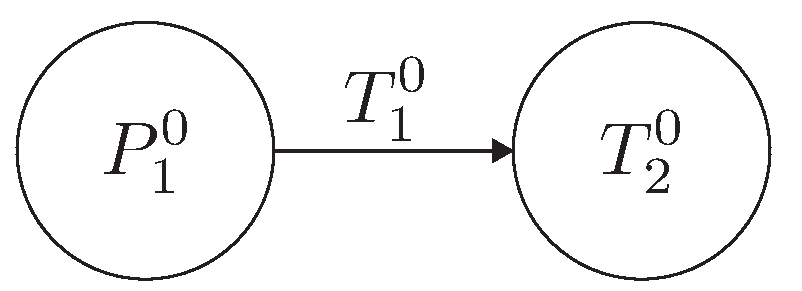
\includegraphics[width=.45\linewidth]{Appendix1/figures/interaction-differentialrotation.pdf}
	\caption{A simple closed interaction diagram. Here a magnetic field $P_1^0$ is acted on by velocity field $T_1^0$ to produce magnetic field $T_2^0$}
	\label{fig:interaction-differentialrotation}
\end{figure}
Another closed interaction diagram is shown in figure \ref{interaction-complicated.pdf}, this is considerably more complicated than figure \ref{fig:interaction-differentialrotation}.
\begin{figure}
	\centering
	\noindent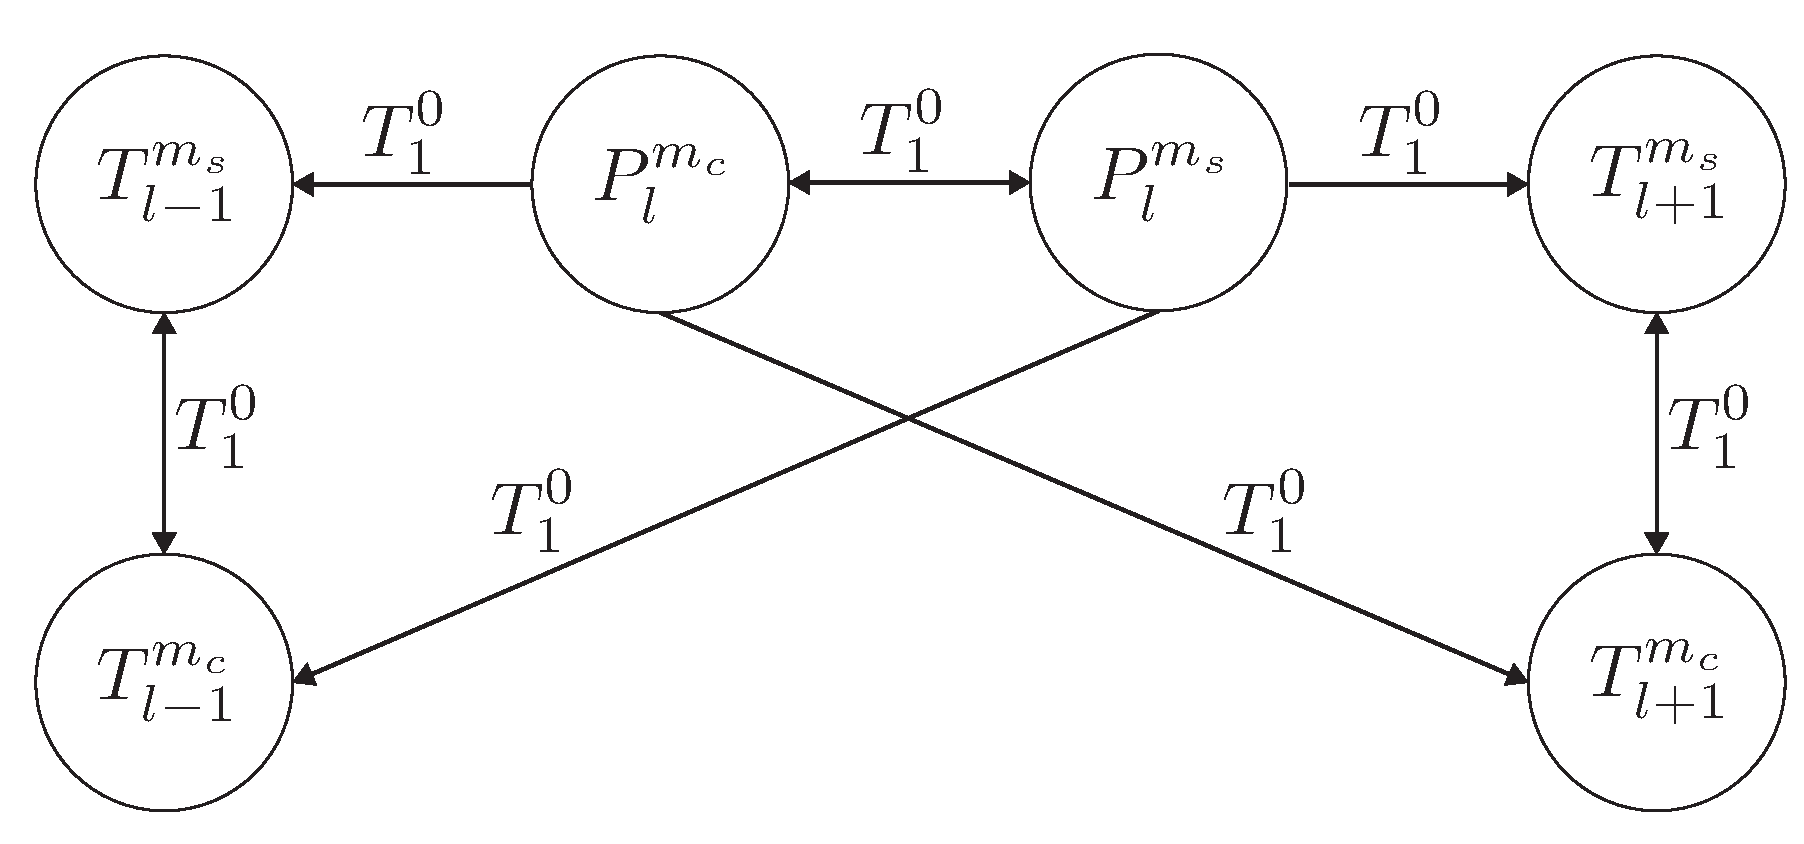
\includegraphics[width=\linewidth]{Appendix1/figures/interaction-complicated.pdf}
	\caption{A more complicated closed interaction diagram. Here a magnetic field $P_1^0$ is acted on by velocity field $T_1^0$ to produce magnetic field $T_2^0$}
	\label{interaction-complicated.pdf}
\end{figure}
Neither of these interaction diagrams represent self-sustaining dynamo as the velocity field is in both is purely toroidal. A purely toroidal velocity field contains no radial component of velocity. This is important because \citet{busse1975} showed that a radial component of the velocity field is a necessary condition for a self sustaining dynamo. 

We have not considered the radial dependence of equations \ref{eq:bgtorexpand4} and \ref{eq:bgpolexpand4} or the boundary conditions associated with them. These details complicate matters somewhat, however an evaluation of the angular terms provides us with a necessary condition for dynamo action which sufficient for the argument we make in chapter \ref{chap:superearth}.

%!TEX root = ../thesis.tex

\chapter{The Local Rossby Number}
\label{chap:rol}
One factor which makes dynamos difficult to understand is the large number of control parameters that are required to specify a solution to the governing equations. This is particularly troubling because the properties of a dynamo is dependent on the values of these control parameters. Unfortunately for numerical reasons dynamo models must be run in a parameter regime for which none of the control parameters is realistic.

\citet{christensen06scaling} developed a scaling law concerning planetary dynamos which has proved to be useful in the prediction of the bulk properties of a dynamo as a function of its control parameters. The Rossby number is normally defined as the ratio of the inertial force to the Coriolis force, from equation \ref{eq:navierstokesgeneralcorlor} this is
\begin{align*}
Ro&=\frac{\rho \mbf{u}\cdot\nabla\mbf{u}}{2\rho\mbf{\Omega}\times\mbf{u}}\\
&\approx\frac{U}{2\Omega L}\\
&\approx\frac{U}{\Omega r_o}.
\end{align*}
\citet{christensen06scaling} noted that while the inertial term depends on the length scale of the flow, the Coriolis term does not. They posited that a better measure of the role rotation plays in a given flow may be a Rossby number which depends on the characteristic length scale of the flow, rather than the characteristic length scale of the container. They defined this length scale as
\begin{equation}
\label{eq:rollength}
\bar{\ell}_{u}=\frac{4Ro_m^2}{\left(1-r_{io}\right)^2}\frac{\sum l\left\langle\mbf{u}_{l}\cdot\mbf{u}_{l}\right\rangle}{2E_{kin}}
\end{equation}
Where $E_{kin}$ is the kinetic energy, defined as
\begin{equation}
E_{kin}=\frac{4 Ro_m^2}{\left(1-r_{io}\right)^{5}}\frac{1}{2}\int_{V}\left(\mbf{u}\cdot\mbf{u}\right)dV
\end{equation}
using the non-dimensionalisation of \citet{kuangandbloxham1999}. Combining these we get
\begin{equation}
\bar{\ell}_{u}=\left(1-r_{io}\right)^{3}\frac{\sum l\left\langle\mbf{u}_{l}\cdot\mbf{u}_{l}\right\rangle}{\int_{V}\left(\mbf{u}\cdot\mbf{u}\right)dV}.
\end{equation}
Since the mean radius to a point inside the shell is of order one, they set the half wavelength of the flow to $\pi/\ell_u$ giving a local Rossby number of 
\begin{equation}
\label{eq:rol}
Ro_{l}=Ro\frac{\bar{\ell}_{u}}{\pi}.
\end{equation}

\citet{christensen06scaling} then noted that the dipole dominance of the poloidal magnetic field depended strongly on the local Rossby number. They showed that dynamo models which had $Ro_{l}\leq 0.12$ had magnetic fields that were predominantly dipolar, while models with $Ro_{l}>0.12$ generated multipolar magnetic fields. This sharp transition is clear if the dipole dominance of the observable magnetic field ($f_{dip}$) is plotted against the local Rossby number (figure \ref{fig:rolfdip}). Using angle brackets to denote a time average, $f_{dip}$ is defined as
\begin{equation}
f_{dip}=\left\langle\frac{ \int_S \sqrt{\mbf{B}_{l=1}\cdot\mbf{B}_{l=1}} }{\sum_{l=1}^{12} \mbf{B}_{l}\cdot\mbf{B}_{l}}\biggr\rvert_{r=r_{o}}\right\rangle
\end{equation}
which is the time average ratio of the r.m.s. amplitude of the dipole field to the r.m.s. amplitude of the field in the first 12 degrees.
\begin{figure}
	\centering
	\noindent\includegraphics[width=.5\linewidth]{Appendix2/figures/fdip.pdf}
	\caption{The dipole dominance ($f_{dip}$) of the observable magnetic field as a function of the local Rossby number. Here $f_{dip}$ is defined as the time average ratio of the r.m.s. amplitude of the dipole field to the r.m.s. amplitude of the field in the first 12 degrees. The Ekman numbers here are in the variables of \citet{christensen06scaling}, they can be converted to the Ekman numbers in this work by multiplying them by a factor of $0.21125$. This figure is reproduced from \citet{christensen06scaling} where it is figure 3.}
	\label{fig:rolfdip}
\end{figure}

Once the local Rossby number is defined, a natural extension is to apply it to the planets of our solar system. The definition of equation \ref{eq:rol} requires a knowledge the characteristic fluid velocity and scale in the fluid outer core. This is very unconstrained for even the Earth, and less well constrained for other planets of our solar system. An alternative approach is to construct scaling laws which relate the control parameters of the dynamo to the local Rossby number. The control parameters depend on the physical properties of the planet (e.g. diffusivities, rotation rates etc.) which are known more accurately than the dynamical properties (i.e. the scale of convection).

Several studies have constructed scaling laws which relate the dynamo control parameters to the local Rossby number \citep{christensen06scaling,OlsonandChristensen2006,aubert2009}. The most general is from \citet{aubert2009}, if it is cast into the non-dimensionalisation used in this work it can be written as
\begin{equation}
Ro_{l}=0.674\frac{1+r_{io}}{\left(1-r_{io}\right)^{-0.64}}p^{0.48}E^{-0.32}q_{\kappa}^{-0.19}.
\label{eq:rolscaling}
\end{equation}
$p$ is the convective power density. Assuming the background state does not change the convective power density can be written as
\begin{equation}
p=\frac{3}{2}\frac{(1-r_{io})^2}{\left(1-r_{io}^3\right)} \left[(1-f_{i})\left(\frac{1}{(1-r_{io})^2}-\frac{3}{5}\frac{\left(1-r_{io}^5\right)}{\left(1-r_{io}^3\right)}\right)+f_{i} \left(\frac{3}{5}\frac{\left(1-r_{io}^5\right)}{\left(1-r_{io}^3\right)}-\frac{r_{io}^2}{(1-r_{io})^2}\right)\right]Ra_Q
\end{equation}
Where $f_i$ is the fraction of the total buoyancy flux injected at the inner core and $Ra_Q$ is a Rayleigh number based on advected buoyancy flux \citep{aubert2009}.

\addcontentsline{toc}{chapter}{Bibliography}
\bibliographystyle{plainnat}
\bibliography{bibliography/bibliography}

\end{document}
